h15223
s 00946/00219/00165
d D 1.2 10/05/12 19:24:01 starck 2 1
c update olivier
e
s 00384/00000/00000
d D 1.1 10/02/18 09:30:29 starck 1 0
c date and time created 10/02/18 09:30:29 by starck
e
u
U
f e 0
t
T
I 1


\chapter{Blind Source Separation on the Sphere}
\label{ch_mrs_ica}

\section{Introduction}
\index{blind source separation}
\index{ICA}

Blind Source Separation (BSS) is a problem that occurs in multi-dimensional data processing. The overall goal is to recover 
D 2
unobserved signals, images or \emph{sources} $S$ from mixtures of these sources $X$ observed typically at the output of an 
E 2
I 2
unobserved signals, images or sources $S$ from mixtures of these sources $X$ observed typically at the output of an 
E 2
array of sensors. The simplest mixture model takes the form:
\begin{equation}\label{model0}
X = A S
\end{equation}
where $X$ and $S$ are random vectors of respective sizes $m \times 1$, $n \times 1$ and $A$ is an $m \times n$ matrix. The 
entries of $S$ are assumed to be independent random variables. Multiplying $S$ by $A$ linearly mixes the $n$ sources into 
$m$ observed processes. \\ 
   
D 2
Independent Component Analysis methods were developed to solve the BSS problem, \emph{i.e.} given a batch of $T$ observed 
E 2
I 2
Independent Component Analysis methods were developed to solve the BSS problem, i.e. given a batch of $T$ observed 
E 2
samples of $X$, estimate the mixing matrix $A$ and reconstruct the corresponding $T$ samples of the source vector $S$, relying 
mostly on the statistical independence of the source processes. Note that with the above model, the independent sources can 
D 2
only be recovered up to a multiplication by a \emph{non-mixing} matrix \emph{i.e.} up to a permutation and a scaling of the 
E 2
I 2
only be recovered up to a multiplication by a non-mixing matrix i.e. up to a permutation and a scaling of the 
E 2
entries of $S$. Although independence is a strong assumption, it is in many cases physically plausible. The point is that 
it goes beyond the simple second order decorrelation obtained for instance using Principal Component Analysis (PCA) : decorrelation 
is not enough to recover the source processes since any rotation of a white random vector remains a white random vector.\\

Algorithms for blind component separation and mixing matrix estimation depend on the model used for the probability distribution 
of the sources~\citep{ica:3easy}. In a first set of techniques, source separation is achieved in a noise-less setting, based on the 
non-Gaussianity of all but possibly one of the components. Most mainstream Independent Component Analysis (ICA)  techniques belong to this category : JADE~\citep{ica:jade}, 
FastICA, Infomax~\citep{ica:icabook}. In a second set of blind techniques, the components are modeled as Gaussian processes, either 
D 2
stationary or non stationary and, in a given representation, separation requires that the sources have diverse, \emph{i.e.} non 
E 2
I 2
stationary or non stationary and, in a given representation, separation requires that the sources have diverse, i.e. non 
E 2
proportional, variance profiles. The Spectral Matching ICA method (SMICA) ~\citep{ica:Del2003}, considers in this sense the case of 
D 2
mixed stationary Gaussian components and goes further than the above model (Eq.~\ref{model0}) by taking into account additive 
\emph{instrumental } noise $N$:
E 2
I 2
mixed stationary Gaussian components and goes further than the above model Eq.~\eqref{model0} by taking into account additive 
instrumental noise $N$:
E 2
\begin{equation}\label{model1}
X = A S + N
\end{equation}
Moving to a Fourier representation, the idea is that colored components can be separated based on the diversity of their power spectra.\\ 
 
The next  section give a short overview of two significant ICA methods mentioned above and implemented in the \mrs package: 
JADE  and FastICA ~\citep{ica:icabook}. 
This is followed by a description of ways to 
combine wavelets and ICA techniques. Some useful properties of wavelet transforms can indeed come enhance the performance of ICA  methods in several situations. 
D 2
Finally, we present a method GMCA, which perform a source compo
E 2
I 2
Finally, we present the method GMCA, which perform a source separation with the use of sparse componenent analysis algorithm.
E 2
    
\section{JADE}
\index{ICA!jade}

The Joint Approximate Diagonalization of Eigenmatrices method (JADE) assumes the observed data $X$ follows the noiseless mixture 
D 2
model~(\ref{model0}) where the independent sources $S$ are non-Gaussian \emph{i.i.d.}\footnote{The letters \emph{i.i.d.} stand for 
E 2
I 2
model~\eqref{model0} where the independent sources $S$ are non-Gaussian i.i.d.\footnote{The letters i.i.d. stand for 
E 2
independently and identically distributed meaning that each entries of $X$ at a given time $t$ are independent of $X$ at any other 
D 2
time $t'$ and that the distribution of $X$ does not depend on time. } random processes. The mixing matrix is assumed to be square 
E 2
I 2
time $t'$ and that the distribution of $X$ does not depend on time.} random processes. The mixing matrix is assumed to be square 
E 2
and invertible so that (de)mixing is actually just a change of basis.

As mentioned above, second order statistics do not retain enough information for source separation in this context: finding a change of 
basis in which the data covariance matrix is diagonal will not in general enable to identify the independent sources properly. Nevertheless, 
D 2
decorrelation is \emph{half the job}~\citep{ica:tutorial} and one may seek the basis in which the data is represented by maximally independent 
E 2
I 2
decorrelation is half the job~\citep{ica:tutorial} and one may seek the basis in which the data is represented by maximally independent 
E 2
processes among those bases in which the data is decorrelated. This leads to so-called orthogonal algorithms: after a proper whitening of 
the data by multiplication with the inverse of a square root of the covariance matrix of the data $W$, one is then seeking a rotation $R$ 
(which leaves things white) so that $\hat{ S}$ defined by
\begin{equation}
\hat{ S} = W^{-1} \, Y =  W^{-1}\, R \, X_{\textrm{white}}  = W^{-1}\, R \, W \, X 
\end{equation}
and $\hat{B} = \widehat{A^{-1}} =  W^{-1}\, R \, W$ are estimations of the sources and of the inverse of the mixing matrix.\\

JADE is such an orthogonal ICA method and, like most mainstream ICA techniques, it exploits higher order statistics so as to achieve some 
D 2
sort of \emph{ non linear decorrelation}. Precisely, in the case of JADE, statistical independence is assessed using fourth order cross cumulants : 
\begin{eqnarray}  \nonumber	 
F_{ijkl} & = & \textrm{cum}( y_i, y_j, y_k, y_l )   \nonumber    \\
  & =& \mathcal{E} (y_i y_j y_k y_l) - \mathcal{E} (y_i y_j)\mathcal{E} (y_k y_l)\nonumber \\
  & & -\mathcal{E} (y_iy_l)\mathcal{E} ( y_j y_k)-\mathcal{E} (y_iy_k)\mathcal{E} (y_j y_k)
E 2
I 2
sort of non linear decorrelation. Precisely, in the case of JADE, statistical independence is assessed using fourth order cross cumulants : 
%\begin{eqnarray} \nonumber	 
%F_{ijkl} & = & \textrm{cum}( y_i, y_j, y_k, y_l ) \nonumber \\
%  & = & \mathcal{E} (y_i y_j y_k y_l) - \mathcal{E} (y_i y_j)\mathcal{E} (y_k y_l) \nonumber \\
%  & & -\mathcal{E} (y_iy_l)\mathcal{E} ( y_j y_k)-\mathcal{E} (y_iy_k)\mathcal{E} (y_j y_k)
%\end{eqnarray}
\begin{eqnarray} \nonumber
F_{ijkl} & = & \textrm{cum}( y_i, y_j, y_k, y_l ) \nonumber \\
 & = & \mathcal{E} (y_i y_j y_k y_l) - \mathcal{E} (y_i y_j)\mathcal{E} (y_k y_l) -\mathcal{E} (y_iy_l)\mathcal{E} ( y_j y_k)-\mathcal{E} (y_iy_k)\mathcal{E} (y_j y_k)
E 2
\end{eqnarray}
where $\mathcal{E}$ stands for statistical expectation and the $y_i$'s are the entries of vector $Y$ modeled as random variables, 
D 2
and the correct change of basis (\emph{i. e.} rotation) is found by somehow \emph{diagonalizing} the fourth order cumulant tensor. 
E 2
I 2
and the correct change of basis (i.e. rotation) is found by somehow diagonalizing the fourth order cumulant tensor. 
E 2
Indeed, if the $y_i$'s were independent, all the cumulants with at least two different indices would be zero. As a consequence of 
D 2
the independence assumption of the source processes $S$ and of the \emph{whiteness} of $Y$ for all rotations $R$, the fourth order 
E 2
I 2
the independence assumption of the source processes $S$ and of the whiteness of $Y$ for all rotations $R$, the fourth order 
E 2
tensor $F$ is well structured: JADE was precisely devised to take advantage of the algebraic properties of $F$. JADE's objective 
function is given by
\begin{eqnarray}  \nonumber	 
%\mathcal{J}_{\textrm{jade}}( R )   &=& \sum _{ijkl \ne ijkk}  \textrm{cum}(  y_i, y_j, y_k, y_l )^2  \nonumber    \\
  \mathcal{J}_{\textrm{jade}}( R ) & =&  \sum _{ij}   \sum_{k \ne l} \textrm{cum}(  y_i, y_j, y_k, y_l )^2  
\end{eqnarray}
which can be interpreted as a joint diagonalization criterion. Fast and robust algorithms are available for the minimization 
of $\mathcal{J}_{\textrm{jade}}( R )$ with respect to $R$ based on Jacobi's method for matrix diagonalization~\citep{ica:pham2001}. 
D 2
More details on JADE can be found in~\citet{ica:jade,ica:tutorial,ica:icabook}.
E 2
I 2
More details on JADE can be found in~\citep{ica:jade,ica:tutorial,ica:icabook}.
E 2


\subsubsection{JADE for spherical maps}

Applying JADE on multichannel data mapped to the sphere does not require any particular modification of the algorithm. Indeed, JADE estimates 
D 2
the fourth order cumulant tensor from the available data samples assuming an \emph{i.i.d.} random field. Hence, given a pixelization scheme on 
E 2
I 2
the fourth order cumulant tensor from the available data samples assuming an i.i.d. random field. Hence, given a pixelization scheme on 
E 2
the sphere such as provided by the Healpix package, JADE can be directly applied to the multichannel spherical data pixels.


\section{FastICA}
\index{ICA!fastica}

FastICA is by now a standard technique in ICA. Like JADE, it is meant for the analysis of mixtures of independent non-Gaussian sources in 
D 2
a noise-less setting. A complete description of this method can be found in \citet{ica:icabook} and references therein. Many papers on this 
algorithm are available at \emph{http://www.cs.helsinki.fi/ u/ahyvarin/papers/fastica.shtml}. We give here a brief and simplified account 
E 2
I 2
a noise-less setting. A complete description of this method can be found in \citep{ica:icabook} and references therein\footnote{Many papers on this 
algorithm are available at http://www.cs.helsinki.fi/u/ahyvarin/papers/fastica.shtml}. We give here a brief and simplified account 
E 2
of the algorithm. FastICA, again like JADE, is a so-called orthogonal ICA method: the independent components are sought by maximizing a 
measure of non-Gaussianity under the constraint that they are decorrelated. Intuitively, one should understand that mixtures of independent 
D 2
non-Gaussian random variables tend to \emph{ look more Gaussian}. An enlightening view on the relation between mutual information, which is 
a natural measure of independence, decorrelation and non-Gaussianity can be found in~\citet{ica:3easy,ica:geomindep}. Non-Gaussianity is assessed 
in FastICA using a contrast function $G$ based on a non-linear approximation to \emph{negentropy}~\citep{ica:icabook}. In practice, depending 
E 2
I 2
non-Gaussian random variables tend to look more Gaussian. An enlightening view on the relation between mutual information, which is 
a natural measure of independence, decorrelation and non-Gaussianity can be found in~\citep{ica:3easy,ica:geomindep}. Non-Gaussianity is assessed 
in FastICA using a contrast function $G$ based on a non-linear approximation to negentropy~\citep{ica:icabook}. In practice, depending 
E 2
on the application, different approximations or non-linear (non-quadratic) functions should be experimented with. In a simple deflation scheme, 
D 2
for sphered data, the directions are found sequentially : a direction $r$ of maximal non-Gaussianity is sought by maximizing 
E 2
I 2
for sphered data, the directions are found sequentially : a direction $r$ of maximal non-Gaussianity is sought by maximizing
E 2
\begin{equation}
J_G(r) = \Big( \mathcal{E} \{ G(r^T x_{\textrm{white}}  ) \} - \mathcal{E} \{ G(\nu ) \} \Big)^2 
\end{equation}
where $\nu$ stands for centered unit variance Gaussian variable, under the constraint that $r$ has unit norm and that $r$ is orthogonal 
D 2
to the directions found previously. The contrast function $G$ can for instance be chosen among the following~\citep{ica:icabook}:
E 2
I 2
to the directions found previously.\\ \\
The contrast function $G$ can for instance be chosen among the following~\citep{ica:icabook}:
E 2
\begin{eqnarray}
G_0 (u)  & = &  \frac{1}{a} \textrm{log}\,\textrm{cosh} (a u ) \nonumber    \\
G_1 (u)  & = &  -\frac{1}{a} \textrm{exp}(- a u^2 / 2 )   \nonumber	   \\
G_2 (u)  & = &  \frac{1}{4} u^4 \nonumber    \\
\end{eqnarray}
where $a$ is a constant to be determined depending on the application. It can be shown that the maxima of $J_G$ occur at certain maxima 
of $\mathcal{E} \{ G(r^T x_{\textrm{white}} ) \} $. These are obtained for $r$ solution to :
\begin{equation}
\mathcal{E} \{ x_{\textrm{white}} g(r^T x_{\textrm{white}}  ) \} - \lambda r = 0 
\end{equation}
where $\lambda$ is a constant easily expressed in terms of the optimal direction $r_0$, and $g$ is the derivative of $G$. Solving this 
D 2
equation using Newton's method, and a few approximations, a \emph{fixed-point} algorithm is derived which consists in repeating the 
E 2
I 2
equation using Newton's method, and a few approximations, a fixed-point algorithm is derived which consists in repeating the 
E 2
following two steps until convergence :
\begin{eqnarray}
r  & \leftarrow & \mathcal{E} \{ x_{\textrm{white}} g(r^T x_{\textrm{white}}  ) \} - \mathcal{E} \{ g'(r^T x_{\textrm{white}}  ) \} r     \nonumber  \\
r  & \leftarrow  &  \frac{r}{\| r \|}   \nonumber	   \\
\end{eqnarray}
A simple implementation of this algorithm is included in the present package. It is largely based on the $\textbf{Matlab}^{TM}$ code 
D 2
available at \emph{www.cis.hut.fi/projects/ica/fastica/}. 
E 2
I 2
available at www.cis.hut.fi/projects/ica/fastica/. 
E 2

 
\section{Wavelet and BSS} 
\index{wavelet!ICA}
\index{ICA!wavelet}

Several properties of wavelets have been recognized as particularly useful in multichannel data processing : bringing wavelets and 
independent component analysis together has proven quite profitable. Extensions WJADE and WSMICA of the two ICA methods described 
previously are discussed in this section.

Wavelets are remarkable at data compression meaning data that is structured in the initial representation requires fewer significant 
coefficients in a wavelet representation. In imprecise and general terms, wavelets grab the coherence between coefficients of the 
structured data and produces a smaller set of significant coefficients which are then less coherent and which have a sparser statistical 
distribution. Then, the super-Gaussian\footnote{A super-Gaussian distribution is also called a lepto-kurtic distribution, referring to a 
D 2
distribution with a narrow central peak and heavy tails. A typical example is the Laplacian distribution.} \emph{i.i.d.} statistical model 
E 2
I 2
distribution with a narrow central peak and heavy tails. A typical example is the Laplacian distribution.} i.i.d. statistical model 
E 2
which appears in most standard ICA methods may better suit the wavelet coefficients of the data than the data samples in the initial representation. 

Wavelets have been developed for the analysis of non-stationary and singular data in order to overcome certain difficulties attached to 
the Fourier transform. Wavelets are widely used to reveal variations in the spectral content of time series or images as they permit to 
single out regions in direct space while retaining localization in the frequency domain. Astrophysical data analysis has much to gain in 
avoiding the assumption of stationarity underlying Fourier analysis. Moreover, observed data maps are commonly imperfectly shaped and 
incomplete with missing or masked patches due to experimental settings, scanning strategies, etc. This will impair direct application of 
the Spectral Matching ICA method described previously. One might consider resorting to wavelets.     
          
 
%In dealing with non stationary data or incomplete data, an attractive feature of  wavelet filters over the spherical harmonic transform is that they are well localized in the initial representation. 

%Dealing with non stationary data or incomplete data is made simpler due to the good localization of wavelet coefficients in the initial representation.In the smaller scales, most of the samples in the filtered signal will  be unaffected by the presence of gaps and only these samples should be used to estimate the data covariance matrices on each wavelet scale.

\subsection*{WJADE and WFastICA}
\label{sec:wjade}
\index{ICA!wjade}
\index{jade!wavelet}

D 2
Wavelets come into play as a sparsifying transform. Applying a wavelet transform on both sides of~(\ref{model0}) does not affect the 
E 2
I 2
Wavelets come into play as a sparsifying transform. Applying a wavelet transform on both sides of~\eqref{model0} does not affect the 
E 2
mixing matrix and the model structure is preserved. Also, moving the data to a wavelet representation does not affect its information 
content. However, the statistical distribution of the data coefficients in the new representation is different: wavelets are known to 
D 2
lead to sparse \emph{i.i.d.} representations of structured data. Further, the \emph{local} (coefficient wise) signal to noise ratio 
E 2
I 2
lead to sparse i.i.d. representations of structured data. Further, the local (coefficient wise) signal to noise ratio 
E 2
depends on the choice of a representation. A wavelet transform tends to grab the informative coherence between pixels while averaging 
D 2
the noise contributions, thus enhancing structures in the data. Although the standard ICA model~(\ref{model0}) is for a noiseless setting, 
the derived methods can be applied to real data. Performance will depend on the detectability of significant coefficients \emph{i.e.} on 
E 2
I 2
the noise contributions, thus enhancing structures in the data. Although the standard ICA model~\eqref{model0} is for a noiseless setting, 
the derived methods can be applied to real data. Performance will depend on the detectability of significant coefficients i.e. on 
E 2
the sparsity of the statistical distribution of the coefficients. Moving to a wavelet representation will often lead to more robustness to noise.    

D 2
Once the data has been transformed to a proper representation (\emph{e.g.} wavelets but also ridgelets and curvelets in the case of strongly 
E 2
I 2
Once the data has been transformed to a proper representation (e.g. wavelets but also ridgelets and curvelets in the case of strongly 
E 2
anisotropic 2D or 3D data), WJADE (resp. WFastICA) consists in applying the standard JADE (resp. FastICA) method to the new multichannel coefficients. Once the mixing matrix 
is estimated, the initial source maps are obtained using the adequate inverse transform after some non linear denoising or thresholding of 
the coefficients if necessary.


\section{Sparse Blind Source Separation: the GMCA method}
% \section{Generalized Morphological Component Analysis on the sphere}
D 2

E 2
\label{sec:gmca}
D 2
\subsection{The GMCA model}
\label{sec:model}
E 2

D 2
The observation with detector $i$ is then a noisy linear mixture of $n$ independent sources $\{s_j\}_{j=1,\cdots,n}$ : 
$x_i = \sum_{j=1}^n a_{ij} s_j + n_i$. The coefficient $a_{ij}$ reflects the emission law of source $s_j$ in the 
frequency band of the $i$-th sensor; $n_i$ models instrumental noise. When $m$ sensors provide observations at 
different frequencies, this linear mixture model can be rewritten in a more convenient matrix formulation :
\begin{equation}
\label{eq:lm_model}
{\bf X} = {\bf AS} + {\bf N}
\end{equation}
where ${\bf X}$ is the $m \times t$ data matrix the rows of which are the observed data maps in each channel, ${\bf A}$ 
is the $m \times n$ mixing matrix, ${\bf S}$ is the $n \times t$ source matrix the rows of which are the sources $s_j$, 
and ${\bf N}$ is the $m \times t$ noise matrix.

We further assume that all the protagonists of the model in Equation~\ref{eq:lm_model} are random components (variables 
or vectors). More particularly, the entries of the noise matrix ${\bf N}$ are assumed to be \textit{independently} 
distributed according to a zero mean Gaussian distribution with variance $\sigma_i^2$ depending on the detector. 
From physical considerations, ${\bf N}$ models instrumental noise the level of which varies independently from one 
detector to another. ${\bf N}$ is thus a random Gaussian variable with zero mean and covariance matrix 
${\bf \Gamma_N} = \mbox{diag}(\sigma_1^2,\cdots,\sigma_m^2)$. In practice, as the detectors are assumed to be accurately calibrated, 
${\bf \Gamma_N}$ is known with high precision. The log-likelihood function is then the following one :
\begin{equation}
\label{eq:ll}
\log P({\bf X} \big| {\bf A},{\bf S},{\bf \Gamma_N}) = -\frac{1}{2} \|{\bf X} - {\bf AS}\|_{2,{\bf \Gamma_N}}^2 + C
\end{equation}
where $C$ is a constant. The notation $\| . \|_{2,{\bf \Gamma_N}}^2$ stands for the Frobenius norm of ${\bf Y}$ in the noise 
covariance metric : $\| Y \|_{2,{\bf \Gamma_N}}^2 = \mbox{ Trace}\left( {\bf Y}^T {\bf \Gamma_N}^{-1} {\bf Y}\right)$. 
From a Bayesian point of view, adding physical priors should help the separation task. We first assume no particular knowledge 
about the emission laws of the components modeled by ${\bf A}$. For simplicity, we consider that each entry of the mixing 
matrix ${\bf A}$ is \textit{i.i.d.}\footnote{Independently and identically distributed.} from a uniform zero mean distribution. 
Note that it would be possible to add some physical constraint on the emission laws reflected in ${\bf A}$.

In the general case, source separation is merely a question of diversity and contrast between the sources (see \citep{Cardo1}). 
For instance, on the one hand JADE relies on non-gaussianity to distinguish between the sources. On the other, SMICA takes advantage 
of the diversity of the mixed components' power spectra to achieve the separation task. ``Non-gaussianity" and ``power spectra diversity" 
are contrasts between the sources. A combination of both characteristics, ``Non-gaussianity" and ``power spectra diversity", 
was also proposed to separate CMB from kinetic SZ signal which are otherwise undistinguishable \citep{forni}. Recent work has 
already emphasized on sparsity as a source of diversity to improve component separation (see \citep{Zibu} and \citep{MMCA}). 
In that setting, each source $\{s_j\}_{j=1,\cdots,n}$ is assumed to be sparse in a representation (potentially overcomplete) $\mathcal{D}$. 
Formally, $\mathcal{D}$ is a fixed dictionary of signal waveforms written as a $T \times t$ matrix. We define the set of projection 
coefficients $\alpha_j$ such that : $\forall j \in \{1,\cdots,n\}, \quad s_j = \alpha_j \mathcal{D}$. Any source $s_j$ is said 
to be sparse in $\mathcal{D}$ if most of the entries of $\alpha_j$ are nearly zero and only a few have ``significant" amplitudes. 
When $\mathcal{D}$ is overcomplete ($T > t$), $\mathcal{D}$ is called a dictionary. Overcomplete representations attractiveness 
in image processing theory leans on their potential to generate very sparse representations of data based on their morphological 
content (see e.g. \cite{DH} and references therein).

In the field of basic source separation we showed in \citep{MMCA} that morphological diversity and sparsity are key properties 
leading to better separation. We noticed that the gist of sparsity-based source separation methods leans on the rationale : 
``\textit{independent sources are distinctly sparse in a dictionary $\mathcal{D}$}". In that study, we considered the simple 
case of morphologically different sources : components were assumed to be sparsely represented in different sub-dictionaries. 
We illustrated that such sparsity prior provides a very effective way to distinguish between sources. In the present paper, 
we focus on a more general setting : the sources can have similar morphologies (\textit{i.e.} all the sources are sparsely 
represented over the whole $\mathcal{D}$). When the overcomplete dictionary $\mathcal{D}$ is made of the union of $D$ orthonormal 
bases (\textit{i.e.} $\mathcal{D} = \left[\Phi_1,\cdots,\Phi_D\right]$) then each source is modeled as the linear combination 
of $D$ so-called morphological components (see \cite{SED} for details on Morphological Component Analysis) - each morphological 
component being sparse in a different orthonormal basis $\{\Phi_1,\cdots,\Phi_D\}$:
\begin{eqnarray}
\forall  j\in \{1,\cdots,n\}, \quad s_j  & = &  \sum_{k=1}^D \varphi_{jk} = \sum_{k=1}^D \alpha_{jk} \Phi_k
\end{eqnarray}
From a statistical viewpoint, we assume that the entries of $\alpha_{jk} = \varphi_{jk}\Phi_k^T$ are \textit{i.i.d} from 
a Laplacian probability distribution with scale parameter $1/\mu$:
\begin{equation}
\label{eq:source_prior}
P(\varphi_{jk}) \propto \exp\left(- \mu \|\varphi_{jk}\Phi_k^T\|_1\right)
\end{equation}
where the $\ell_1$-norm $\|.\|_1$ stands for $\|x\|_1 = \sum_{p=1}^t |x[p]|$ in which $x[p]$ is the $p$-th entry of $x$. In practice, 
the Laplacian prior is well adapted to model leptokurtic sparse signals. We classically assume that the morphological components are 
statistically mutually independent : $P({\bf S}) = \prod_{j,k} P(\varphi_{jk})$. Estimating the sources ${\bf S}$ is then equivalent 
to estimating the set of morphological components $\{\varphi_{jk}\}_{j=1,\cdots,n;k=1,\cdots,D}$. In this Bayesian context, we propose 
to estimate those morphological components $\{\varphi_{jk}\}$ and the mixing matrix ${\bf A}$ from a \textit{maximum a posteriori} (MAP) 
leading to the following optimization problem:
\begin{equation}
\left\{\{\hat{\varphi}_{jk}\},{\bf \hat{A}}\right\} = {\arg\max}_{\{\varphi_{jk}\},{\bf A}} P({\bf X}|{\bf A},\{\varphi_{jk}\},{\bf \Gamma_N}) \prod_{j,k}P(\varphi_{jk}) P({\bf A})
\end{equation}
where we further assumed that the morphological components $\{\varphi_{jk}\}$ are independent of ${\bf A}$. Owing to Equations~\ref{eq:ll} 
and \ref{eq:source_prior}, the mixing matrix ${\bf A}$ and the morphological components $\{\varphi_{jk}\}$ are obtained by minimizing 
the following negative log \textit{a posteriori}:
\begin{equation}
\label{eq:optim}
\left\{\{\hat{\varphi}_{jk}\},{\bf \hat{A}}\right\} = {\arg\min}_{\{\varphi_{jk}\},{\bf A}}\|{\bf X} - {\bf AS}\|_{2,{\bf \Gamma_N}}^2 + 2 \mu \sum_{j=1}^n \sum_{k=1}^D \|\varphi_{jk}\Phi_k^T\|_1
\end{equation}
where $\forall j \in \{1,\cdots,n\},\quad s_j = \sum_{k=1}^D \varphi_{jk}$. Equation~\ref{eq:optim} leads to the GMCA estimates 
of the sources and the mixing matrix in a general sparse component separation context. Interestingly, in the case of CMB data, 
the sources we look for (CMB, galactic dust and SZ) are quite sparse in the same unique orthonormal wavelet basis. The dictionary
$\mathcal{D}$ then reduces to a single orthonormal basis $\Phi$. In that case, since $\Phi$ is unitary, Equation~\ref{eq:optim} 
can be rewritten as follows :
\begin{eqnarray}
\label{eq:foptim}
\left\{{\bf \hat{\alpha}},{\bf \hat{A}}\right\} &=& {\arg\min}_{{\boldsymbol \alpha},{\bf A}} \|{\bf X}\Phi^T - {\bf A\alpha}\|_{2,{\bf \Gamma_N}}^2 + 2 \mu \|{\boldsymbol \alpha}\|_1 \nonumber \\
						&=& {\arg\min}_{{\boldsymbol \alpha},{\bf A}} f_\mu({\boldsymbol \alpha},{\bf A}) = {\arg\min}_{{\boldsymbol \alpha},{\bf A}} f_0({\bf A}, {\boldsymbol \alpha}) + 2\mu f_1({\boldsymbol \alpha})
\end{eqnarray}
where ${\boldsymbol \alpha} = {\bf S}\Phi^T$. Note that the estimation is done in the sparse representation $\Phi$ requiring a single 
transform of the data ${\bf X}\Phi^T$. To remain computationally efficient, GMCA relies on practical transforms which generally involve 
fast implicit operators (typical complexity of $\mathcal{O}\left(t\right)$ or $\mathcal{O}\left(t \log t \right)$). In \citet{Zibu}, 
the authors also used a unique orthonormal wavelet basis. While a gradient descent is used in \cite{Zibu}, we use a fast and efficient 
iterative thresholding optimization scheme which we describe in the next section.

\subsection{Solving the optimization problem}
\label{sec:algo}
The \textit{maximum a posteriori} estimates of the coefficients ${\boldsymbol \alpha}$ and the mixing matrix in Equation~\ref{eq:foptim} 
lead to a non-convex minimization problem. Note that in Equation~\ref{eq:foptim} the functional to be minimized suffers from several 
invariances : any permutation or rescaling of the sources and the mixing matrix leaves the product $\bf A{\boldsymbol \alpha}$ unaltered. 
The scale invariance is computationally alleviated by forcing the columns of ${\bf A}$ to have unit $\ell_2$ norm~: $\forall i\in{1,\cdots,n},\quad a^{i^T}a^i = 1$ 
where $a^i$ is the $i$-th column of ${\bf A}$. 

As solutions of problem~(\ref{eq:foptim}) have no explicit formulation, we propose solving it by means of a block-coordinate relaxation 
iterative algorithm such that each iteration $(h)$ is decomposed into two steps : (i) estimation of the sources ${\bf S}$ assuming the 
mixing matrix is fixed to its current estimate ${\bf \hat{A}}^{(h-1)}$ and (ii) estimation of the mixing matrix assuming the sources are 
fixed to their current estimates ${\bf \hat{S}}^{(h)}$. It is not difficult to see that the objective MAP functional in (\ref{eq:foptim}) 
is continuous on its effective domain and has compact level sets. Moreover, this objective function is convex in the source coefficient 
vectors $(\alpha_1,\ldots,\alpha_n)$, and $f_0$ has an open domain, is continuous and G\^ateaux differentiable. Thus by \cite[Theorem 4.1]{Tseng2001}, 
the iterates generated by our alternating algorithm are defined and bounded, and each accumulation point is a stationary point of the MAP 
functional. In other words, our iterative algorithm will converge. Hence, at iteration $(h)$, the sources are estimated from a \textit{maximum a posteriori} 
assuming ${\bf A} = {\bf \hat{A}}^{(h-1)}$. By classical ideas in convex analysis, a necessary condition for ${\boldsymbol \alpha}$ to be 
a minimizer is that the zero is an element of the subdifferential of the objective at ${\boldsymbol \alpha}$. We calculate\footnote{For clarity, 
we drop the upper script $(h-1)$ and write $\hat{\bf A} = \hat{\bf A}^{(h-1)}$.}:
\begin{equation}
\label{eq:subdiff}
\partial_{\boldsymbol \alpha} f_\mu({\boldsymbol \alpha},{\bf A})= -2{\bf {\bf A}}^T{\bf \Gamma_N}^{-1}({\bf X}\Phi^T - {\bf A}{\boldsymbol \alpha}) + 2\mu \partial_{\boldsymbol \alpha} \|{\boldsymbol \alpha}\|_1
\end{equation}
where $\partial_{\boldsymbol \alpha} \|{\boldsymbol \alpha}\|_1$ is defined as (owing to the separability of the prior):
\[
\partial_{\boldsymbol \alpha} \|{\boldsymbol \alpha}\|_1 = \left\{U \in \mathbb{R}^{n \times t} \Bigg| 
\begin{array}{ccc}
U{j,k} & = \mbox{ sign}(\alpha_{j,k}), & ~ \alpha_{j,k} \neq 0 \\
U{j,k} & \in [-1,1], & ~ \alpha_{j,k} = 0
\end{array} \right\}.
\]
Hence, Equation \ref{eq:subdiff} can be rewritten equivalently as two conditions leading to the following (proximal) fixed point equation:
\begin{equation}
\label{eq:it_estim1}
\begin{array}{cc}
\hat{\alpha}_{j,k} = 0, & \text{if} ~ \left|{\left({\bf A}^T{\bf \Gamma_N}^{-1}{\bf X}\Phi^T\right)}_{j,k} \right| \leq \mu \\
{\bf {\bf A}}^T{\bf \Gamma_N}^{-1}({\bf X}\Phi^T - {\bf A}\hat{\boldsymbol \alpha}) = \mu \mbox{ sign}\left(\hat{\boldsymbol \alpha}\right), & \text{otherwise}. 
\end{array}
\end{equation}
Unfortunately, Equation~\ref{eq:it_estim1} has no closed-form solution in general. It must be iterated and is thus computationally demanding. 
Fortunately, it can be simplified when ${\bf A}$ has nearly orthogonal columns in the noise covariance matrix (\textit{i.e.} 
${\bf \hat{A}}^T{\bf \Gamma_N}^{-1}{\bf \hat{A}} \simeq \mbox{diag}\left({\bf \hat{A}}^T{\bf \Gamma_N}^{-1}{\bf \hat{A}}\right)$). 
Let ${\bf C} = {\left({\bf \hat{A}}^T{\bf \Gamma_N}^{-1}{\bf \hat{A}}\right)}^{-1}{\bf A}^T{\bf \Gamma_N}^{-1}{\bf X}\Phi^T$, Equation~\ref{eq:it_estim1} 
boils down to the following set of equations $\forall j\in\{1,\cdots,n\}$:
\begin{equation}
\label{eq:it_estim}
\begin{array}{ccc}
\hat{\alpha}_{j,k} & = 0, \quad \text{if} ~ \left|{{\bf C}}_{j,k} \right| \leq \mu^{(h)} \sigma_j^2 \\
\hat{\alpha}_j & = {\left[{\bf C}\right]}_j - \mu \sigma_j^2  \mbox{ sign}\left(\hat{\alpha}_j\right), \quad \text{otherwise}.
\end{array}
\end{equation}
where $[{\bf Y}]_j$ is the $j$-th row of ${\bf Y}$. In practice, even if the approximation we make is not strictly valid, such a simplification 
leads to good computational results. These equations are known as soft-thresholding with threshold $\mu^{(h)} \sigma_j^2$. We define $\mathrm{ST}_{\delta}(.)$, 
the soft-thresholding operator with threshold $\delta$. At iteration $(h)$, the sources are thus estimated such that:
\begin{equation}
\hat{\alpha}_j^{(h)} = \mathrm{ST}_{\mu^{(h)} \sigma_j^2}\left(\left[{\bf C}\right]_j\right)
\end{equation}
The $j$th source is reconstructed as $\hat{s}_j^{(h)} = \hat{\alpha}_j^{(h)}\Phi$. The mixing matrix ${\bf A}$ is then estimated by a maximum 
likelihood estimate amounting to a simple least-squares update assuming ${\bf S}$ is fixed. The GMCA algorithm is then described as follows :
\begin{flushleft}
\vspace{0.15in}
\centering
\begin{tabular}{|c|} \hline
\begin{minipage}[h]{0.95\linewidth}
\vspace{0.025in} \footnotesize{\textsf{1. Set the number of iterations $I_{\max}$ and thresholds $\delta_j^{(0)} = \mu^{(0)}\sigma_j^2$\\} 
\textsf{2. While each $\mu^{(h)}$ is higher than a given lower bound $\mu_{min}$ (e.g. can depend on the noise variance), \\}
\hspace{0.1in} \textsf{-- Proceed with the following iteration to estimate source coefficients ${\boldsymbol \alpha}$ at iteration $h$ assuming ${\bf A}$ is fixed:}
\hspace{0.2in} \textsf{$\hat{\alpha}_j^{(h)} = \mathrm{ST}_{\mu^{(h)} \sigma_j^2}\left(\left[{\left({\bf \hat{A}}^T{\bf \Gamma_N}^{-1}{\bf \hat{A}}\right)}^{-1}{\bf \hat{A}}^T{\bf \Gamma_N}^{-1}{\bf X}\Phi^T\right]_j\right)$:\\}
\hspace{0.1in} \textsf{-- Update $\bf A$ assuming ${\boldsymbol \alpha}$ is fixed :}
\hspace{0.2in} \textsf{${\bf \hat{A}}^{(h)} = {\bf X}\Phi^T{\bf \hat{\boldsymbol \alpha}}^T\left({\bf \hat{\boldsymbol \alpha}}{\bf \hat{\boldsymbol \alpha}}^T\right)^{-1}$\\}
\textsf{-- Decrease the threshold $\mu^{(h)}$ following a given strategy}}
\vspace{0.05in}
\end{minipage}
\\\hline
\end{tabular}
\vspace{0.15in}
\end{flushleft}
Note that the overall optimization scheme is based on an iterative and alternate thresholding algorithm involving a 
\textit{coarse to fine} estimation process. Indeed, \textit{coarse} versions of the sources (\textit{i.e.} containing 
the most ``significant" features of the sources) are first computed with high values of $\mu^{(h)}$.
E 2
I 2
\subsection{Morpho-Spectral Diversity}
%\label{sec:morph-spec-diversity}
Extending the redundant representation framework to the multichannel case requires defining what a multichannel overcomplete representation is.
Let us assume in this section that $\A = [\varphi_{\nu,1}, \cdots, \varphi_{\nu, N_c}] \in \RR^{N_c \times N_s}$ is a \textit{known spectral} dictionary, 
and $\W = [ \varphi_{1}, \cdots, \varphi_{T}] \in \RR^{N \times T}$ is a \textit{spatial} or \textit{temporal} dictionary\footnote{The adjectives 
\textit{spectral} and \textit{spatial} that characterize the dictionaries are not formal. Owing to the symmetry of the multichannel sparse decomposition problems, 
$\A$ and $\W$ have no formal difference. In practice and more particularly in multi/hyperspectral imaging, $\A$ will refer to the dictionary of physical spectra 
and $\W$ to the dictionary of image/signal waveforms. In the BSS problem, $\A$ is unknown.}. We assume that each source $s_i$ can be represented as 
a (sparse) linear combination of atoms in $\W$; $s_i=\W\alpha_i$. Let $\balpha$ the $N_s \times T$ matrix whose rows are $\alpha_i^\Tr$.

From Eq.~\eqref{model0}, the multichannel noiseless data $\bY$ can be written as
\be
\label{eq:tensor1}
\bY = \A\balpha\W^\Tr = \sum_{i=1}^{N_s}\sum_{j=1}^{T} \parenth{\varphi_{\nu,i}\varphi_{j}^\Tr}\alpha_i[j] ~.
\ee
Consequently, each column in of $\bY$ reads
\be
\label{eq:tensor2}
\bY[.,l] = \parenth{\A \otimes \W[l,.]} \mathrm{vect}(\balpha) ~, \quad \forall ~ l=1,\cdots,N ~,
\ee
and finally
\be
\label{eq:tensor3}
\mathrm{vect}(\bY) = \parenth{\A \otimes \W} \mathrm{vect}(\balpha) ~,
\ee
where $\otimes$ is the tensor (Kronecker) product and the operator $\mathrm{vect}$ stacks the columns of its argument in a long 1D vector. 
This latter equation brings a clear and simple insight: the sparsity of the sources in $\W$ translates into sparsity of the multichannel data 
$\bY$ in the multichannel tensor product dictionary ${\bf \Psi}=\A \otimes \W$. This concept of multichannel dictionary has also been noted in \citep{GN05}.

The multichannel dictionary $\bf \Psi$ can also be seen as concatenation of multichannel atoms ${\bf \Psi}^{(ij)}=\varphi_{\nu,i}\varphi_{j}^\Tr$ 
which are rank-one matrices obtained from each atomic spectrum $\varphi_{\nu,i}$ and each spatial elementary atom $\varphi_{j}$ (see Eq.~\eqref{eq:tensor1}). 

Some of the popular recovery results in sparse component analysis algorithm rely on the mutual coherence of 
the dictionary~\citep{cur:elad02,miki:Gribonval-Nielsen,mca:Donoho-Elad}. In the multichannel case a quantity 
of that kind can be defined. In fact, by standard properties of the tensor product, one can easily show that 
the Gram matrix of a tensor product is the tensor product of the Gram matrices. Thus the mutual coherence of the multichannel dictionary $\bf \Psi$ is:
\index{coherence}
\begin{equation}
\label{eq:mmc}
0 \le \mu_{\bf \Psi}  =  \max\left\{\mu_{\A},\mu_{\W}\right\} < 1 ~ .
\end{equation}

This expression of mutual coherence is instructive as it tells us that multichannel atoms can be distinguished 
based on their spatial or spectral morphology. In other words, discriminating two multichannel atoms $\Psi_{ij}$ and $\Psi_{i'j'}$ may put on different faces:
\begin{itemize}
\item{Spatial or temporal (respectively spectral) diversity:} in this case $i=i'$ and $j \neq j'$ (respectively $i \neq i'$ and $j = j'$). 
These atoms have the same spectrum (respectively, spatial shape) but one can discriminate between them based on their 
spatial (respectively, spectral) diversity. From \eqref{eq:mmc}, their coherence is lower than $\mu_{{\W}}$ (respectively $\mu_{{\A}}$). 
Disentangling these multichannel atoms can equivalently be done in \ref{ch_sca_datarest}.

\item{Both diversities:} $i \neq i'$ and $j \neq j'$, this seems to be a more favorable scenario to differentiate 
the atoms as they do not share neither the same spectrum nor the same spatial (or temporal) ``shape". Note that 
from \eqref{eq:mmc}, the coherence between these atoms in this case is lower than $\mu_{{\A}}\mu_{{\W}} \le \max\left\{\mu_{\A},\mu_{\W}\right\}$.
\end{itemize}

\subsection{Multichannel Sparse Decomposition}

We embark from Eq.~\eqref{eq:tensor1}, where the multichannel dictionary ${\bf \Psi}$ is supposed to be overcomplete, i.e. $NN_c < TN_s$. 
The goal is to recover the sparsest solution $\balpha$ from $\bY$ which requires solving:
\begin{equation}
\label{eq:multi_l0}
\min_{\balpha \in \RR^{N_s \times T}} \sum_{i=1}^{N_s}\norm{\alpha_i}_{0} \st \bY  = \A \balpha \W^\Tr.
\end{equation}
As justified in \ref{sect_mca}, this combinatorial problem can be replaced by its convex relaxation substituting the $\ell_1$ norm for the $\ell_0$ pseudo-norm, hence giving:
\begin{equation}
\label{eq:multi_l1}
\min_{\balpha \in \RR^{N_s \times T}} \sum_{i=1}^{N_s}\norm{\alpha_i}_{1} \st \bY  = \A \balpha \W^\Tr.
\end{equation}

As \eqref{eq:tensor3} is a vectorized monochannel form of \eqref{eq:tensor1}, what we are trying so do is actually to find 
the sparsest solution of a monochannel underdetermined system of linear equations where the solution is sparse in an 
overcomplete tensor product dictionary. Recovery properties of monochannel sparse decomposition by $\ell_1$ minimization 
were overviewed in chapter~\ref{ch_sca_datarest}. Therefore, if one is able to translate those identifiability criteria 
in the language of tensor product dictionaries, then we are done.

In particular, the coherence-based sparse recovery criterion given in \citep{DonohoHuo} is trivial to adapt owing to \eqref{eq:mmc}. 
Indeed, if $\bY$ is $k$-sparse in the multichannel dictionary ${\bf \Psi}$ with $k < C(\mu_{{\bf \Psi}}^{-1}+1)$ for some $C > 0$ (typically $C=1/2$), 
and the dictionary is sufficiently incoherent (both spectrally and spatially), then the solution of Eq.~\eqref{eq:multi_l1} is unique, 
is a point of equivalence of Eq.~\eqref{eq:multi_l0} and Eq.~\eqref{eq:multi_l1}, and the recovery is stable to bounded noise on $\bY$. 

Above, we addressed the multichannel sparse decomposition problem without assuming any constraint on the sparsity pattern 
of the different channels. It is worth however pointing out that sparse recovery conditions from multichannel measurements 
can be refined if some structured sparsity is hypothesized. For instance, for structured multichannel representation 
(e.g. sources with disjoint supports) \citep{GN05} provided coherence-based sufficient recovery conditions by solving Eq.~\eqref{eq:multi_l1}. 
One should note that despite apparent similarities, the multichannel sparse decomposition problem discussed here is conceptually 
different from the one targeting \textit{simultaneous} sparse recovery of multiple measurements vectors (MMV) considered by several authors, see e.g. 
\citep{CREK05,MalioutovMMV05,TroppMMV06,ChenHuo06,ArgyriouMMVLearning08,BachMMVLearning08,GribonvalMMV08,EldarMMV08,LouniciMMVLearning09,WainwrightMMV09}. 
The latter are not aware of any mixing process via $\A$, and their goal is to recover $\balpha$ from MMV $\bY=\balpha\W^\Tr$ in which 
the vectors $\alpha_i$, i.e. rows of $\balpha$, have a common sparsity pattern. However the MMV model can also be written 
$\mathrm{vect}(\bY^\Tr) = \parenth{\W \otimes \I} \mathrm{vect}(\balpha^\Tr)$ as in Eq.~\eqref{eq:tensor3}. The most widely used approach 
to solve the simultaneous sparse recovery problem with joint sparsity is to minimize a mixed $\ell_p-\ell_q$ norm of the form 
$\sum_{j=1}^T\parenth{\norm{\balpha[.,j]}_p^q}^{1/q}$ for $p \geq 1, 0 \leq q \leq +\infty$.

\subsection{Generalized Morphological Component Analysis}
\label{subsec:gmca}
We now turn to the BSS problem and highlight the role of sparsity and morphological diversity as a source of contrast to solve it. 
Towards this goal, we assume that the sources are sparse in the spatial dictionary $\W$ that is the concatenation of $K$ orthonormal bases 
$\parenth{{\W}_{k}}_{k=1,\cdots,K}$: $\W = \left[{\W}_{1},\cdots,{\W}_{K} \right]$. The restriction to orthonormal bases is only formal 
and the algorithms to be presented later still work in practice even with redundant sub-dictionaries $\W_k$. 

\newpage
The Generalized Morphological Component Analysis framework assumes a priori that each source is modeled as the linear combination 
of $K$ morphological components where each component is sparse in a specific basis:
\begin{eqnarray}
\label{eq:sourcecomponents}
\forall i \in \{1,\cdots,N_s\}; \qquad s_i & = & \sum_{k=1}^K x_{i,k} = \sum_{k=1}^K \W_k\alpha_{i,k} \\
& = & \W \alpha_i \qquad \mbox{ where } \alpha_i =  \left[\alpha_{i,1}^\Tr,\cdots,\alpha_{i,K}^\Tr \right]^\Tr ~ \nonumber
\end{eqnarray}
GMCA seeks an unmixing scheme, through the estimation of $\A$, which leads to the sparsest sources $\bf S$ in the dictionary $\W$. 
This is expressed by the following optimization problem written in the augmented Lagrangian form:
\begin{multline}
\label{eq:optimgmca}
\min_{{\A},\alpha_{1,1},\cdots,\alpha_{N_s,K}} \frac{1}{2}\norm{\bY - {\A}\balpha\W^\Tr}^2_{\mathrm{F}} + \lambda \sum_{i=1}^{N_s} \sum_{k=1}^K \norm{\alpha_{i,k}}_p^p \\ 
\st \norm{a_i}_2 = 1 ~ \forall i \in \{1,\cdots,N_s\} ~
\end{multline} 
where typically $p=0$ or its relaxed convex version with $p=1$, and $\norm{{\bf X}}_{\mathrm{F}}=\parenth{\trace({\bf X}^\Tr{\bf X})}^{1/2}$ is the Frobenius norm. 
The unit $\ell_2$-norm constraint on the columns of $\A$ avoids the classical scale indeterminacy of the product $\bf AS$ in \eqref{model1}. 
The reader may have noticed that the MCA problem in chapter~\ref{ch_sca_datarest} is a special case of the GMCA problem Eq.~\eqref{eq:optimgmca} 
when there is only one source $N_s=1$ and one channel $N_c=1$ (no mixing). Thus GMCA is indeed a multichannel generalization of MCA. 

The program \eqref{eq:optimgmca} is a notoriously difficult non-convex optimization problem even for convex penalties when $p \geq 1$. 
More conveniently, following \eqref{model0}, the product $\bf AS$ can be split into $N_s \cdot K$ multichannel morphological components: 
${\bf AS} = \sum_{i,k} a_i x_{i,k}^\Tr = \sum_{i,k} (a_i \alpha_{i,k}^\Tr) \W_k^\Tr$. Based on this decomposition, and inspired by 
the block-coordinate relaxation as for MCA, GMCA yields an alternating minimization algorithm to estimate iteratively one term at a time \citep{starck:bobin07}. 
We will show shortly that the estimation of each morphological component $x_{i,k} = \W_k\alpha_{i,k}$ assuming $\A$ and $x_{\{i',k'\} \neq \{i,k\} }$ 
are fixed is obtained by simple hard or soft thresholding for $p=0$ and $p=1$.

Define the $(i,k)^{\textrm{th}}$ multichannel marginal residual by:
\begin{equation}
\label{eq:gmca_resi}
{\bf R}_{i,k} = {\bY} - \sum_{i' \neq i}   \sum_{k'\neq k}    a_{i'} x_{i',k'}^\Tr ~
\end{equation} 
as the part of the data $\bY$ unexplained by the multichannel morphological component $a_i x_{i,k}^\Tr$. Estimating $x_{i,k} = \W_{k} \alpha_{i,k}$, 
assuming $\A$ and the other components $x_{(i',k') \neq (i,k)}$ are fixed, leads to the component-wise optimization problem:
\begin{equation}
\label{eq:componentwisephi}
\min_{x_{i,k} \in \RR^{N}} \frac{1}{2}\norm{{\bf R}_{i,k} - (a_i \alpha_{i,k}^\Tr)\W^\Tr}_{\mathrm{F}}^2 +  \lambda \norm{\alpha_{i,k}}_p^p ~
\end{equation}

Since here ${\W}_k$ is an orthogonal matrix, with calculations using proximity operators, it can be shown that the unique solution 
of Eq.~\eqref{eq:componentwisephi} is obtained by a hard ($p=0$) or soft ($p=1$) thresholding. Hence, the closed-form estimate of 
the morphological component $x_{i,k}$ is: 
\begin{equation}
\label{eq:st_update}
\tilde{x}_{i,k} = \Delta_{\W_k,\lambda^\prime} \parenth{\frac{1}{\norm{a_i}_2^2} {\bf R}_{i,k}^\Tr a_i} ~
\end{equation}
where $\lambda^\prime=\lambda/\norm{a_i}_2^2$ for soft thresholding and $\lambda^\prime=\sqrt{2\lambda}/{\norm{a_i}_2}$ for hard thresholding. 
The operator $\Delta_{{\bf D}, \lambda}(x)$ consists of (i) computing the coefficients of $x$ in the dictionary ${\bf D}$, (ii)
thresholding (soft or hard) the obtained coefficients with the threshold $\lambda$, and (iii) reconstructing from thresholded coefficients: 
\begin{equation}
\Delta_{{\bf D},\lambda}(x) = {\bf D} \Thres_{\lambda} \left( {\bf D}^\Tr x \right)
\end{equation}
$\Thres_{\lambda}$ is either a hard or a soft thresholding. When $\W_k$ is redundant, \eqref{eq:st_update} is only the first iteration 
of a forward-backward splitting recursion, and which should be used when $\W_k$ is overcomplete.
However in practice \eqref{eq:st_update} can still be used to save computation time.
\index{iterative!hard thresholding}
\index{iterative!soft thresholding}

Now, considering $\{a_{i'}\}_{i' \neq i}$ and all morphological components as fixed, and recalling that $N_c \geq N_s$, updating the column $a_i$ is then just a least-squares estimate
\begin{equation}
\label{eq:a_update}
\tilde{a}_i = \frac{1}{\norm{s_i}^2_2} \left({\bf Y} - \sum_{i' \neq i} a_{i'} s_{i'}^\Tr\right) s_i ~
\end{equation}
where $s_i = \sum_{k=1}^K x_{i,k}$. This estimate is then projected onto the unit sphere to meet the unit $\ell_2$-norm constraint in Eq.~\eqref{eq:optimgmca}.
The GMCA algorithm is summarized in Algorithm~\ref{algo_gmca}.

{\linespread{1}
\begin{algorithm}[htb]
\caption{GMCA algorithm.}
\label{algo_gmca}
\noindent{\bf Task:} Sparse Blind Source Separation.\\
\noindent{\bf Parameters:} The data $\bY$, the dictionary $\W=[\W_1 \cdots \W_K]$, number of iterations $\niter$, number of sources $N_s$ and channels $N_c$, stopping threshold $\lambda_{\min}$, threshold update schedule.\\
\noindent{\bf Initialization:} $x_{i,k}^{(0)} = 0$ for all $(i,k)$, $\A^{(0)}$ random and threshold $\lambda_0$.\\
\noindent{\bf Main iteration:} \\
\For{$t=1$ {\bf to} $\niter$}{
    \For{$i=1,\cdots,N_s$ }{
    \For{$k=1,\cdots,K$ }{
       Compute the marginal residuals: $${\bf R}_{i,k}^{(t)} = {\bY}- \sum_{(i',k') \neq (i,k)} {a}_{i'}^{{(t-1)}}{x}_{i',k'}^{{(t-1)}^\Tr}.$$
       Estimate the current component ${x}_{i,k}^{(t)}$ via thresholding with threshold $\lambda_t$:\\
       ${x}_{i,k}^{(t)} = \Delta_{\W_k, \lambda_t}\left({\bf R}_{i,k}^{{(t)}^\Tr}{a}_i^{{{(t-1)}}}\right)$.
    }
Update $i$th source $s_i^{(t)} = \sum_{k=1}^K x_{ik}^{(t)}$. \\
Update $a_i$ assuming $a_{i' \neq i}^{(t)}$ and the morphological components $ {x}_{i,k}^{(t)} $ are fixed~:\\
 $ {a}_i^{{(t)}} = \frac{1}{\|{s}_i^{(t)}\|_2^2} \left({\bY} - \sum_{i' \neq i}^{N_s} {a}_{i'}^{(t-1)} {s}_{i'}^{{(t)}^\Tr} \right){s}_i^{{(t)}}$ and normalize to a unit $\ell_2$ norm.
}
Update the threshold $\lambda_t$ according to the given schedule.\\
\lIf{$\lambda_t \leq \lambda_{\min}$} stop.
}
\noindent{\bf Output:} Estimated sources $\big(s^{(\niter)}_i\big)_{i=1,\cdots,N_s}$ and mixing matrix ${\A}^{(\niter)}$.
\end{algorithm}}

For $p=1$ and fixed threshold $\lambda$, Algorithm~\ref{algo_gmca} can be shown to converge to a stationary point, see \citep{Tseng01,bobin-gmca-cmb}. 
This point is not guaranteed to be even a local minimum of the energy, and this is even less clear for $p=0$. Thus, in the same vein as MCA, GMCA relies 
on a salient-to-fine strategy using a varying threshold to mitigate the problem of sensitivity to initialization. More precisely, GMCA first computes 
coarse versions of the morphological components for any fixed source $s_i$. These raw sources are estimated from their most significant coefficients in $\W$. 
Then, the corresponding column $a_i$ is estimated from the most significant features of $s_i$. Each source and its corresponding column of $\A$ are then 
alternately and progressively refined as the threshold decreases towards $\lambda_{\min}$. This particular iterative thresholding scheme provides robustness 
to noise and initialization by working first on the most significant features in the data and then progressively incorporating smaller details to finely 
tune the model parameters. GMCA can be used with either linear or exponential decrease of the threshold as for MCA.

If $\A$ were known and fixed, the GMCA would be equivalent to performing an MCA sparse decomposition of $\bY$ in the tensor product 
multichannel dictionary ${\A} \otimes \W$. But as GMCA also updates the mixing matrix at each iteration, it is able to learn the 
spectral part of the multichannel dictionary directly from the data.

\subsubsection{The Thresholding Strategy}

\index{iterative!hard thresholding}
\index{iterative!soft thresholding}

\paragraph*{Hard or soft thresholding?} In practice, it was observed that hard thresholding leads to better results \citep{starck:bobin06,starck:bobin07}. 
Furthermore, if $\A$ is known and no noise contaminates the data, GMCA with hard thresholding will enjoy the sparse recovery guarantees given in \citep{starck:bobin_2,BobinJMIV}, 
with the proviso that the morphological components are contrasted and sparse in a sufficiently incoherent multichannel dictionary ${\A} \otimes \W$. 
%Furthermore in \citet{starck:bobin_2}, it was shown empirically that the use of hard-thresholding is likely to provide the $\ell_0$ sparse solution for 
%the single channel sparse decomposition problem. By analogy, the use of a hard-thresholding operator is assumed to solve the multichannel $\ell_0$ quasi-norm 
%problem instead of \eqref{eq:optim_l1}. Recent results give also theoretical support to iterative hard thresholding methods \citep{blumensath08,blumensath09,maleki09,donoho09}.

\paragraph*{Handling additive Gaussian noise.}
The GMCA algorithm is well suited to deal with data contaminated with additive Gaussian noise (see the next section for a Bayesian interpretation). 
For instance, assume that the noise $\bf E$ in \eqref{model1} is additive white Gaussian in each channel, i.e. its covariance matrix 
${\boldsymbol \Sigma}_{\bf E}$ is diagonal, and let $\sigma_{\bf E}$ be its standard deviation supposed equal for all channels for simplicity. 
Then, Algorithm~\ref{algo_gmca} can be applied as described above with $\lambda_{\min}=\tau\sigma_{\bf E}$, where $\tau$ is chosen as in denoising methods, 
typically taking its value in the range $[3,4]$. This attribute of GMCA makes it a suitable choice for use in noisy BSS. 
GMCA not only manages to separate the sources, but also succeeds in removing additive noise as a by-product.

\subsection{The Bayesian Perspective}
GMCA can be interpreted from a Bayesian standpoint. For instance, let us assume that the entries of the mixtures $\parenth{y_i}_{i=1,\cdots,N_c}$, 
the mixing matrix $\A$, the sources $\parenth{s_i}_{i=1,\cdots,N_s}$ and the noise matrix $\bf E$ are random processes. We assume that the noise 
$\bf E$ is zero-mean Gaussian where the noise vector $\veps_i$ in each channel is white, but the noise between channels is possibly correlated with 
known covariance matrix ${\boldsymbol \Sigma}_{\bf E}$. This means that the log-likelihood function takes the form:
\begin{equation}
LL(\bY\big|{\bf S},{\A},{\boldsymbol \Sigma}_{\bf E}) = \frac{1}{2} \norm{{\bY} - {\bf{AS}}}_{{\boldsymbol \Sigma}_{\bf E}}^2 ~,\ \text{where} \norm{\bf X}_{{\boldsymbol \Sigma}_{\bf E}}^2 = \trace\big({\bf X}^\Tr{\boldsymbol \Sigma}_{\bf E}^{-1}{\bf X}\big)
\end{equation}

We further assume that the uniform prior is imposed on entries of $\A$. Other priors on $\A$ could be imposed; e.g. known fixed column for example. 
As far as the sources are concerned, they are known from \eqref{eq:sourcecomponents} to be sparse in the dictionary $\W$. Thus their coefficients 
$\balpha=[\alpha_1,\cdots,\alpha_{N_s}]^\Tr$ will be assumed as drawn independently from a leptokurtic PDF with heavy tails 
such as the generalized Gaussian distribution form:
\begin{multline}
\label{eq:indepas}
\qquad \pdf_{\balpha}(\alpha_{1,1},\ldots,\alpha_{N_s,K}) \propto \prod_{i=1}^{N_s}\prod_{k=1}^{K}\exp\parenth{-\lambda_{i,k}\norm{\alpha_{i}}_{p_{i,k}}^{p_{i,k}}} ~ \\
0 \leq p_{i,k} < 2 ~ \forall (i,k) \in \{1,\cdots,N_s\}\times\{1,\cdots,K\} ~
\end{multline}
Putting together the log-likelihood function and the priors on $\A$ and $\balpha$, the MAP estimator leads to the following optimization problem:
\begin{equation}
\label{eq:optim_bayes}
\min_{{\A},\alpha_{1,1},\cdots,\alpha_{N_s,K}} \frac{1}{2}\norm{\bY - {\A}\balpha\W^\Tr}^2_{{\boldsymbol \Sigma}_{\bf E}} + \sum_{i=1}^{N_s} \sum_{k=1}^K \lambda_{i,k}\norm{\alpha_{i,k}}_{p_{i,k}}^{p_{i,k}} ~
\end{equation}
This problem has strong similarity with that of Eq.~\eqref{eq:optimgmca}. More precisely, if the noise is homoscedastic and decorrelated between channels 
(i.e. ${\boldsymbol \Sigma}_{\bf E} = \sigma_{\bf E}^2 {{\bf I}}$), if the shape parameters $p_{i,k}$ of the generalized Gaussian distribution prior 
are all equal to $p$ and the scale parameters are all taken as $\lambda_{i,k}=\lambda/\sigma_{\bf E}^2$, and if the columns of $\A$ are assumed uniform 
on the unit sphere, then Eq.~\eqref{eq:optim_bayes} is exactly Eq.~\eqref{eq:optimgmca}. Note that in the development above, the independence assumption in \eqref{eq:indepas} 
does not necessarily entail independence of the sources. Rather it means that there are no a priori assumptions that indicate any dependency between the sources. 

\subsection{The Fast GMCA Algorithm}
\label{gmca_algo}
\label{fast_gmca}
The goal here is to speed up the GMCA algorithm. As a warm-up, assume that the dictionary ${\W}$ is no longer redundant and reduces to a single orthobasis (i.e. $K=1$). 
Let us denote $\Ya=\bY\W$ the matrix where each of its rows stores the coefficients of each channel $y_i$. The optimization problem Eq.~\eqref{eq:optimgmca} then becomes 
(we omit the $\ell_2$ constraint on $\A$ to lighten the notation):
\begin{equation}
\label{eq:optim2}
\min_{{\A},{\bf \balpha}} \frac{1}{2}\norm{\Ya - {\A} \balpha}_\mathrm{F}^2 + \lambda \sum_{i=1}^{N_s} \norm{\alpha_{i}}_p^p ~
\end{equation}
where $p=0$ or $p=1$. The GMCA algorithm no longer needs to apply the analysis and synthesis operators at each iteration as only the channels $\bY$ 
have to be transformed once in $\W$. Clearly, this case is computationally much cheaper. 

However, this is rigorously valid only for an orthobasis dictionary, and no orthonormal basis is able to sparsely represent large variety of signals 
and yet we would like to use very sparse signal representations which motivated the use of redundancy in the first place. Arguments supporting the 
substitution of \eqref{eq:optim2} for \eqref{eq:optimgmca} for a redundant dictionary ${\W}$ were given in \citep{starck:bobin07,bobin08_aiep}. The idea is to first 
compute the sparsest representation of each channel $y_i$ in the redundant dictionary $\W$ using an appropriate (non-linear) decomposition algorithm (e.g. BP, MCA). 
Now, $\Ya$ denotes the matrix where each row contains the sparse decomposition of the corresponding channel. Because the channels are linear mixtures 
of the sources via the mixing matrix $\A$, the key argument developed by \citep{starck:bobin07} is that the sparse decomposition algorithm must preserve linear mixtures. 
Descriptively, the sparsest decomposition provided by the algorithm when applied to each channel must be equal to the linear combination of the sparsest 
decompositions of the sources. This statement is valid if the sources and the channels are identifiable, meaning that they verify sufficient conditions 
so that their unique sparsest representation can be recovered by the decomposition algorithm. For instance, if MCA is used, then it is sufficient as in 
\citep{starck:bobin_2,BobinJMIV} that the channels and the sources be sparse enough in an incoherent dictionary $\W$, and their morphological components 
be sufficiently contrasted. See \citep{starck:bobin07,bobin08_aiep} for details.

Hence, under these circumstances, a fast GMCA algorithm can be designed to solve \eqref{eq:optim2} by working in the transform domain after decomposing each 
observed channel $y_i$ in ${\W}$ using a sparse decomposition algorithm such as MCA. There is an additional important simplification when substituting problem 
\eqref{eq:optim2} for \eqref{eq:optimgmca}. Indeed, since $N_c \geq N_s$ (i.e. overdetermined BSS), it turns out that \eqref{eq:optim2} is a multichannel overdetermined 
least-squares fit with $\ell_0/\ell_1$-sparsity penalization. We again use an alternating minimization scheme to solve for $\A$ and $\balpha$:
\index{iterative!hard thresholding}
\index{iterative!soft thresholding}
\begin{itemize}
\item Update the coefficients: when $\A$ is fixed, since the quadratic term is strictly convex ($\A$ has full column-rank), the marginal optimization problem 
can be solved by a general form of the forward-backward splitting iteration \citep{ChenRockafellar97}:
\begin{equation}
\balpha^{(t+1)} = \Thres_{\mu\lambda} \parenth{\balpha^{(t)} + \mu{\boldsymbol \Xi} \A^\Tr(\Ya - {\A}\balpha^{(t)})} ~
\end{equation}
where ${\boldsymbol \Xi}$ is a relaxation matrix such that the spectral radius of $({\bf I} - \mu{\boldsymbol \Xi}\A^\Tr\A)$ is bounded above by 1, 
and the step-size $0 < \mu \leq 1/\opnorm{{\boldsymbol \Xi}\A\A^\Tr}$. Taking ${\boldsymbol \Xi} = (\A^\Tr\A)^{-1}$ ($\A^\Tr\A$ is non-singular 
and a kind of Newton's method ensues) yields the closed-form
\begin{equation}
\tilde{\balpha}  =  \Thres_{\lambda}\parenth{\A^{+}\Ya}
\end{equation}
where $\Thres_{\lambda}$ is a thresholding operator (hard for $p=0$ and soft for $p=1$).
\item If $\balpha$ is fixed, and since $\balpha$ is full row-rank, the mixing matrix $\A$ is given by the least-squares estimate: 
\begin{equation}
{\bf \tilde{A}} = \Ya\balpha^\Tr\parenth{\balpha\balpha^\Tr}^{-1} = \Ya\balpha^+ ~
\end{equation}
and the columns of ${\bf \tilde{A}}$ are then normalized.
\end{itemize}
Note that the latter two-step estimation scheme has a flavor of the alternating sparse coding/dictionary learning algorithm presented by \citep{ksvd:elad,fadili:peyrespie07} in a different framework.

This two-stage iterative process leads to the accelerated version of GMCA summarized in Algorithm~\ref{algo_fast_gmca}.
{\linespread{1}
\begin{algorithm}[htb]
\caption{Fast GMCA algorithm.}
\label{algo_fast_gmca}
\noindent{\bf Task:} Sparse Blind Source Separation.\\
\noindent{\bf Parameters:} The data $\bY$, the dictionary $\W=[\W_1 \cdots \W_K]$, number of iterations $\niter$, number of sources $N_s$ and channels $N_c$, 
stopping threshold $\lambda_{\min}$, threshold update schedule.\\
\noindent{\bf Initialization:} 
\begin{itemize}
\item $\balpha^{(0)} = 0$,  $\A^{(0)}$ a random matrix.
\item Apply the MCA Algorithm~\ref{algo_mca} with $\W$ to each data channel $y_i$ to get $\Ya$.
\item Set threshold $\lambda_0 = \max_{i,l}\abs{\Ya[i,l]}$.
\end{itemize}
\noindent{\bf Main iteration:} \\
\For{$t=1$ {\bf to} $\niter$}{
\begin{itemize}
\item  Update the coefficients $\balpha$:
      ${\balpha}^{(t+1)} =  \Thres_{\lambda_t}\big({\A}^{(t)^+} \Ya\big)$.
\item  Update the mixing matrix $\A$:
      ${\A}^{(t+1)} =   \Ya\balpha^{(t+1)^+}$, normalize columns to a unit $\ell_2$ norm.
\item Update  the threshold $ \lambda_t$ according to the given schedule.
\end{itemize}
\lIf{$\lambda_t \leq \lambda_{\min}$} stop.
}
Reconstruct the sources: $\tilde{s}_i   =    \sum_{k=1}^K {\W}_{k}  \alpha^{(\niter)}_{i,k}, i=1,\cdots,N_s$.\\
\noindent{\bf Output:} Estimated sources $\big(\tilde{s}_i\big)_{i=1,\cdots,N_s}$ and mixing matrix ${\A}^{(\niter)}$.
\end{algorithm}}

In the same vein as in Section~\ref{subsec:gmca}, the coarse-to-fine process is also at the heart of this fast version of GMCA 
with the threshold that decreases with increasing iteration count. This again brings robustness to noise and initialization.


%\subsection{The GMCA model}
%\label{sec:model}
%
%The observation with detector $i$ is then a noisy linear mixture of $n$ independent sources $\{s_j\}_{j=1,\cdots,n}$ : 
%$x_i = \sum_{j=1}^n a_{ij} s_j + n_i$. The coefficient $a_{ij}$ reflects the emission law of source $s_j$ in the 
%frequency band of the $i$-th sensor; $n_i$ models instrumental noise. When $m$ sensors provide observations at 
%different frequencies, this linear mixture model can be rewritten in a more convenient matrix formulation :
%\begin{equation}
%\label{eq:lm_model}
%{\bf X} = {\bf AS} + {\bf N}
%\end{equation}
%where ${\bf X}$ is the $m \times t$ data matrix the rows of which are the observed data maps in each channel, ${\bf A}$ 
%is the $m \times n$ mixing matrix, ${\bf S}$ is the $n \times t$ source matrix the rows of which are the sources $s_j$, 
%and ${\bf N}$ is the $m \times t$ noise matrix.
%
%We further assume that all the protagonists of the model in Equation~\ref{eq:lm_model} are random components (variables 
%or vectors). More particularly, the entries of the noise matrix ${\bf N}$ are assumed to be \textit{independently} 
%distributed according to a zero mean Gaussian distribution with variance $\sigma_i^2$ depending on the detector. 
%From physical considerations, ${\bf N}$ models instrumental noise the level of which varies independently from one 
%detector to another. ${\bf N}$ is thus a random Gaussian variable with zero mean and covariance matrix 
%${\bf \Gamma_N} = \mbox{diag}(\sigma_1^2,\cdots,\sigma_m^2)$. In practice, as the detectors are assumed to be accurately calibrated, 
%${\bf \Gamma_N}$ is known with high precision. The log-likelihood function is then the following one :
E 2
%\begin{equation}
D 2
%\forall j\in\{1,\cdots,n\},\quad \hat{s}_j = \mathrm{ST}_{\mu^{(h)} \sigma_j^2}\left({\left({\bf \hat{A}}^T{\bf \Gamma_N}^{-1}{\bf \hat{A}}\right)}^{-1}{\bf \hat{A}}^T{\bf \Gamma_N}^{-1}{\bf X}\Phi^T\right)\Phi
E 2
I 2
%\label{eq:ll}
%\log P({\bf X} \big| {\bf A},{\bf S},{\bf \Gamma_N}) = -\frac{1}{2} \|{\bf X} - {\bf AS}\|_{2,{\bf \Gamma_N}}^2 + C
E 2
%\end{equation}
D 2
In the early stages of the algorithm, the mixing matrix is then estimated from the most ``significant" features of the sources 
which are less perturbed by noise. The estimation of ${\bf A}$ and ${\bf S}$ is then refined at each iteration as $\mu^{(h)}$ 
(and thus the thresholds $\{\mu^{(h)}\sigma_j^2\}_{j=1,\cdots,n}$) decreases towards a final value $\mu_{min}$. We already used 
this minimization scheme in \cite{MMCA} where this optimization process provided robustness and helped convergence even in a 
noisy context. Experiments in Section~\ref{sec:results} illustrate that it achieves good results with GMCA as well.
E 2
I 2
%where $C$ is a constant. The notation $\| . \|_{2,{\bf \Gamma_N}}^2$ stands for the Frobenius norm of ${\bf Y}$ in the noise 
%covariance metric : $\| Y \|_{2,{\bf \Gamma_N}}^2 = \mbox{Trace}\left( {\bf Y}^T {\bf \Gamma_N}^{-1} {\bf Y}\right)$. 
%From a Bayesian point of view, adding physical priors should help the separation task. We first assume no particular knowledge 
%about the emission laws of the components modeled by ${\bf A}$. For simplicity, we consider that each entry of the mixing 
%matrix ${\bf A}$ is \textit{i.i.d.}\footnote{Independently and identically distributed.} from a uniform zero mean distribution. 
%Note that it would be possible to add some physical constraint on the emission laws reflected in ${\bf A}$.
%
%In the general case, source separation is merely a question of diversity and contrast between the sources (see \citep{Cardo1}). 
%For instance, on the one hand JADE relies on non-gaussianity to distinguish between the sources. On the other, SMICA takes advantage 
%of the diversity of the mixed components' power spectra to achieve the separation task. ``Non-gaussianity" and ``power spectra diversity" 
%are contrasts between the sources. A combination of both characteristics, ``Non-gaussianity" and ``power spectra diversity", 
%was also proposed to separate CMB from kinetic SZ signal which are otherwise undistinguishable \citep{forni}. Recent work has 
%already emphasized on sparsity as a source of diversity to improve component separation (see \citep{Zibu} and \citep{MMCA}). 
%In that setting, each source $\{s_j\}_{j=1,\cdots,n}$ is assumed to be sparse in a representation (potentially overcomplete) $\mathcal{D}$. 
%Formally, $\mathcal{D}$ is a fixed dictionary of signal waveforms written as a $T \times t$ matrix. We define the set of projection 
%coefficients $\alpha_j$ such that : $\forall j \in \{1,\cdots,n\}, \quad s_j = \alpha_j \mathcal{D}$. Any source $s_j$ is said 
%to be sparse in $\mathcal{D}$ if most of the entries of $\alpha_j$ are nearly zero and only a few have ``significant" amplitudes. 
%When $\mathcal{D}$ is overcomplete ($T > t$), $\mathcal{D}$ is called a dictionary. Overcomplete representations attractiveness 
%in image processing theory leans on their potential to generate very sparse representations of data based on their morphological 
%content (see e.g. \citep{DH} and references therein).
%
%In the field of basic source separation we showed in \citep{MMCA} that morphological diversity and sparsity are key properties 
%leading to better separation. We noticed that the gist of sparsity-based source separation methods leans on the rationale : 
%``\textit{independent sources are distinctly sparse in a dictionary $\mathcal{D}$}". In that study, we considered the simple 
%case of morphologically different sources : components were assumed to be sparsely represented in different sub-dictionaries. 
%We illustrated that such sparsity prior provides a very effective way to distinguish between sources. In the present paper, 
%we focus on a more general setting : the sources can have similar morphologies (\textit{i.e.} all the sources are sparsely 
%represented over the whole $\mathcal{D}$). When the overcomplete dictionary $\mathcal{D}$ is made of the union of $D$ orthonormal 
%bases (\textit{i.e.} $\mathcal{D} = \left[\Phi_1,\cdots,\Phi_D\right]$) then each source is modeled as the linear combination 
%of $D$ so-called morphological components (see \citep{SED} for details on Morphological Component Analysis) - each morphological 
%component being sparse in a different orthonormal basis $\{\Phi_1,\cdots,\Phi_D\}$:
%\begin{eqnarray}
%\forall j\in \{1,\cdots,n\}, \quad s_j & = & \sum_{k=1}^D \varphi_{jk} = \sum_{k=1}^D \alpha_{jk} \Phi_k
%\end{eqnarray}
%From a statistical viewpoint, we assume that the entries of $\alpha_{jk} = \varphi_{jk}\Phi_k^T$ are \textit{i.i.d} from 
%a Laplacian probability distribution with scale parameter $1/\mu$:
%\begin{equation}
%\label{eq:source_prior}
%P(\varphi_{jk}) \propto \exp\left(- \mu \|\varphi_{jk}\Phi_k^T\|_1\right)
%\end{equation}
%where the $\ell_1$-norm $\|.\|_1$ stands for $\|x\|_1 = \sum_{p=1}^t |x[p]|$ in which $x[p]$ is the $p$-th entry of $x$. In practice, 
%the Laplacian prior is well adapted to model leptokurtic sparse signals. We classically assume that the morphological components are 
%statistically mutually independent : $P({\bf S}) = \prod_{j,k} P(\varphi_{jk})$. Estimating the sources ${\bf S}$ is then equivalent 
%to estimating the set of morphological components $\{\varphi_{jk}\}_{j=1,\cdots,n;k=1,\cdots,D}$. In this Bayesian context, we propose 
%to estimate those morphological components $\{\varphi_{jk}\}$ and the mixing matrix ${\bf A}$ from a \textit{maximum a posteriori} (MAP) 
%leading to the following optimization problem:
%\begin{equation}
%\left\{\{\hat{\varphi}_{jk}\},{\bf \hat{A}}\right\} = {\arg\max}_{\{\varphi_{jk}\},{\bf A}} P({\bf X}|{\bf A},\{\varphi_{jk}\},{\bf \Gamma_N}) \prod_{j,k}P(\varphi_{jk}) P({\bf A})
%\end{equation}
%where we further assumed that the morphological components $\{\varphi_{jk}\}$ are independent of ${\bf A}$. Owing to Equations~\ref{eq:ll} 
%and \ref{eq:source_prior}, the mixing matrix ${\bf A}$ and the morphological components $\{\varphi_{jk}\}$ are obtained by minimizing 
%the following negative log \textit{a posteriori}:
%\begin{equation}
%\label{eq:optim}
%\left\{\{\hat{\varphi}_{jk}\},{\bf \hat{A}}\right\} = {\arg\min}_{\{\varphi_{jk}\},{\bf A}}\|{\bf X} - {\bf AS}\|_{2,{\bf \Gamma_N}}^2 + 2 \mu \sum_{j=1}^n \sum_{k=1}^D \|\varphi_{jk}\Phi_k^T\|_1
%\end{equation}
%where $\forall j \in \{1,\cdots,n\},\quad s_j = \sum_{k=1}^D \varphi_{jk}$. Equation~\ref{eq:optim} leads to the GMCA estimates 
%of the sources and the mixing matrix in a general sparse component separation context. Interestingly, in the case of CMB data, 
%the sources we look for (CMB, galactic dust and SZ) are quite sparse in the same unique orthonormal wavelet basis. The dictionary
%$\mathcal{D}$ then reduces to a single orthonormal basis $\Phi$. In that case, since $\Phi$ is unitary, Equation~\ref{eq:optim} 
%can be rewritten as follows :
%\begin{eqnarray}
%\label{eq:foptim}
%\left\{{\bf \hat{\alpha}},{\bf \hat{A}}\right\} &=& {\arg\min}_{{\boldsymbol \alpha},{\bf A}} \|{\bf X}\Phi^T - {\bf A\alpha}\|_{2,{\bf \Gamma_N}}^2 + 2 \mu \|{\boldsymbol \alpha}\|_1 \nonumber \\
%						&=& {\arg\min}_{{\boldsymbol \alpha},{\bf A}} f_\mu({\boldsymbol \alpha},{\bf A}) = {\arg\min}_{{\boldsymbol \alpha},{\bf A}} f_0({\bf A}, {\boldsymbol \alpha}) + 2\mu f_1({\boldsymbol \alpha})
%\end{eqnarray}
%where ${\boldsymbol \alpha} = {\bf S}\Phi^T$. Note that the estimation is done in the sparse representation $\Phi$ requiring a single 
%transform of the data ${\bf X}\Phi^T$. To remain computationally efficient, GMCA relies on practical transforms which generally involve 
%fast implicit operators (typical complexity of $\mathcal{O}\left(t\right)$ or $\mathcal{O}\left(t \log t \right)$). In \citep{Zibu}, 
%the authors also used a unique orthonormal wavelet basis. While a gradient descent is used in \citep{Zibu}, we use a fast and efficient 
%iterative thresholding optimization scheme which we describe in the next section.
%
%\subsection{Solving the optimization problem}
%\label{sec:algo}
%The \textit{maximum a posteriori} estimates of the coefficients ${\boldsymbol \alpha}$ and the mixing matrix in Equation~\ref{eq:foptim} 
%lead to a non-convex minimization problem. Note that in Equation~\ref{eq:foptim} the functional to be minimized suffers from several 
%invariances : any permutation or rescaling of the sources and the mixing matrix leaves the product $\bf A{\boldsymbol \alpha}$ unaltered. 
%The scale invariance is computationally alleviated by forcing the columns of ${\bf A}$ to have unit $\ell_2$ norm~: $\forall i\in{1,\cdots,n},\quad a^{i^T}a^i = 1$ 
%where $a^i$ is the $i$-th column of ${\bf A}$. 
%
%As solutions of problem~(\ref{eq:foptim}) have no explicit formulation, we propose solving it by means of a block-coordinate relaxation 
%iterative algorithm such that each iteration $(h)$ is decomposed into two steps : (i) estimation of the sources ${\bf S}$ assuming the 
%mixing matrix is fixed to its current estimate ${\bf \hat{A}}^{(h-1)}$ and (ii) estimation of the mixing matrix assuming the sources are 
%fixed to their current estimates ${\bf \hat{S}}^{(h)}$. It is not difficult to see that the objective MAP functional in (\ref{eq:foptim}) 
%is continuous on its effective domain and has compact level sets. Moreover, this objective function is convex in the source coefficient 
%vectors $(\alpha_1,\ldots,\alpha_n)$, and $f_0$ has an open domain, is continuous and G\^ateaux differentiable. Thus by \cite[Theorem 4.1]{Tseng2001}, 
%the iterates generated by our alternating algorithm are defined and bounded, and each accumulation point is a stationary point of the MAP 
%functional. In other words, our iterative algorithm will converge. Hence, at iteration $(h)$, the sources are estimated from a \textit{maximum a posteriori} 
%assuming ${\bf A} = {\bf \hat{A}}^{(h-1)}$. By classical ideas in convex analysis, a necessary condition for ${\boldsymbol \alpha}$ to be 
%a minimizer is that the zero is an element of the subdifferential of the objective at ${\boldsymbol \alpha}$. We calculate\footnote{For clarity, 
%we drop the upper script $(h-1)$ and write $\hat{\bf A} = \hat{\bf A}^{(h-1)}$.}:
%\begin{equation}
%\label{eq:subdiff}
%\partial_{\boldsymbol \alpha} f_\mu({\boldsymbol \alpha},{\bf A})= -2{\bf {\bf A}}^T{\bf \Gamma_N}^{-1}({\bf X}\Phi^T - {\bf A}{\boldsymbol \alpha}) + 2\mu \partial_{\boldsymbol \alpha} \|{\boldsymbol \alpha}\|_1
%\end{equation}
%where $\partial_{\boldsymbol \alpha} \|{\boldsymbol \alpha}\|_1$ is defined as (owing to the separability of the prior):
%\[
%\partial_{\boldsymbol \alpha} \|{\boldsymbol \alpha}\|_1 = \left\{U \in \mathbb{R}^{n \times t} \Bigg| 
%\begin{array}{ccc}
%U{j,k} & = \mbox{ sign}(\alpha_{j,k}), & ~ \alpha_{j,k} \neq 0 \\
%U{j,k} & \in [-1,1], & ~ \alpha_{j,k} = 0
%\end{array} \right\}.
%\]
%Hence, Equation \ref{eq:subdiff} can be rewritten equivalently as two conditions leading to the following (proximal) fixed point equation:
%\begin{equation}
%\label{eq:it_estim1}
%\begin{array}{cc}
%\hat{\alpha}_{j,k} = 0, & \text{if} ~ \left|{\left({\bf A}^T{\bf \Gamma_N}^{-1}{\bf X}\Phi^T\right)}_{j,k} \right| \leq \mu \\
%{\bf {\bf A}}^T{\bf \Gamma_N}^{-1}({\bf X}\Phi^T - {\bf A}\hat{\boldsymbol \alpha}) = \mu \mbox{ sign}\left(\hat{\boldsymbol \alpha}\right), & \text{otherwise}. 
%\end{array}
%\end{equation}
%Unfortunately, Equation~\ref{eq:it_estim1} has no closed-form solution in general. It must be iterated and is thus computationally demanding. 
%Fortunately, it can be simplified when ${\bf A}$ has nearly orthogonal columns in the noise covariance matrix (\textit{i.e.} 
%${\bf \hat{A}}^T{\bf \Gamma_N}^{-1}{\bf \hat{A}} \simeq \mbox{diag}\left({\bf \hat{A}}^T{\bf \Gamma_N}^{-1}{\bf \hat{A}}\right)$). 
%Let ${\bf C} = {\left({\bf \hat{A}}^T{\bf \Gamma_N}^{-1}{\bf \hat{A}}\right)}^{-1}{\bf A}^T{\bf \Gamma_N}^{-1}{\bf X}\Phi^T$, Equation~\ref{eq:it_estim1} 
%boils down to the following set of equations $\forall j\in\{1,\cdots,n\}$:
%\begin{equation}
%\label{eq:it_estim}
%\begin{array}{ccc}
%\hat{\alpha}_{j,k} & = 0, \quad \text{if} ~ \left|{{\bf C}}_{j,k} \right| \leq \mu^{(h)} \sigma_j^2 \\
%\hat{\alpha}_j & = {\left[{\bf C}\right]}_j - \mu \sigma_j^2  \mbox{ sign}\left(\hat{\alpha}_j\right), \quad \text{otherwise}.
%\end{array}
%\end{equation}
%where $[{\bf Y}]_j$ is the $j$-th row of ${\bf Y}$. In practice, even if the approximation we make is not strictly valid, such a simplification 
%leads to good computational results. These equations are known as soft-thresholding with threshold $\mu^{(h)} \sigma_j^2$. We define $\mathrm{ST}_{\delta}(.)$, 
%the soft-thresholding operator with threshold $\delta$. At iteration $(h)$, the sources are thus estimated such that:
%\begin{equation}
%\hat{\alpha}_j^{(h)} = \mathrm{ST}_{\mu^{(h)} \sigma_j^2}\left(\left[{\bf C}\right]_j\right)
%\end{equation}
%The $j$th source is reconstructed as $\hat{s}_j^{(h)} = \hat{\alpha}_j^{(h)}\Phi$. The mixing matrix ${\bf A}$ is then estimated by a maximum 
%likelihood estimate amounting to a simple least-squares update assuming ${\bf S}$ is fixed. The GMCA algorithm is then described in \ref{algo_gmca}:
%
%%\begin{flushleft}
%%\vspace{0.15in}
%%\centering
%%\begin{tabular}{|c|} \hline
%%\begin{minipage}[h]{0.95\linewidth}
%%\vspace{0.025in} \footnotesize{\textsf{1. Set the number of iterations $I_{\max}$ and thresholds $\delta_j^{(0)} = \mu^{(0)}\sigma_j^2$\\} 
%%\textsf{2. While each $\mu^{(h)}$ is higher than a given lower bound $\mu_{min}$ (e.g. can depend on the noise variance), \\}
%%\hspace{0.1in} \textsf{-- Proceed with the following iteration to estimate source coefficients ${\boldsymbol \alpha}$ at iteration $h$ assuming ${\bf A}$ is fixed:}
%%\hspace{0.2in} \textsf{$\hat{\alpha}_j^{(h)} = \mathrm{ST}_{\mu^{(h)} \sigma_j^2}\left(\left[{\left({\bf \hat{A}}^T{\bf \Gamma_N}^{-1}{\bf \hat{A}}\right)}^{-1}{\bf \hat{A}}^T{\bf \Gamma_N}^{-1}{\bf X}\Phi^T\right]_j\right)$:\\}
%%\hspace{0.1in} \textsf{-- Update $\bf A$ assuming ${\boldsymbol \alpha}$ is fixed :}
%%\hspace{0.2in} \textsf{${\bf \hat{A}}^{(h)} = {\bf X}\Phi^T{\bf \hat{\boldsymbol \alpha}}^T\left({\bf \hat{\boldsymbol \alpha}}{\bf \hat{\boldsymbol \alpha}}^T\right)^{-1}$\\}
%%\textsf{-- Decrease the threshold $\mu^{(h)}$ following a given strategy}}
%%\vspace{0.05in}
%%\end{minipage}
%%\\\hline
%%\end{tabular}
%%\vspace{0.15in}
%%\end{flushleft}
%
%{\linespread{1}
%\begin{algorithm}[h]
%\caption{The Generalized Morphological Component Analysis algorithm.}
%\label{algo_gmca}
%\noindent{\bf Task:} Compute the GMCA of a discrete $X$.\\
%\noindent{\bf Parameters:} Data samples $X$, number of estimated sources $J$, dictionnary $\Phi$, noise covariance matrix ${\bf \Gamma_N}$.\\
%\noindent{\bf Initialization:}
%\begin{itemize}
%\item Set the number of iterations $I_{\max}$
%\item Set the initial thresholds $\delta_j^{(0)} = \mu^{(0)}\sigma_j^2$
%\item Set the final thresholds $\mu_{\min}$, it can depend on the noise standard deviation
%\end{itemize}
%\While{ $\mu^{(h)}_{j} > \mu_{\min}$ }{
%\begin{enumerate}[1.]
%\item estimate source coefficients ${\boldsymbol \alpha}$ at iteration $h$ assuming ${\bf A}$ is fixed :
%
%\lFor{$j = 1, \cdots, J$}{ $\hat{\alpha}_j^{(h)} = \mathrm{ST}_{\mu^{(h)} \sigma_j^2}\left(\left[{\left({\bf \hat{A}}^T{\bf \Gamma_N}^{-1}{\bf \hat{A}}\right)}^{-1}{\bf \hat{A}}^T{\bf \Gamma_N}^{-1}{\bf X}\Phi^T\right]_j\right)$ }
%\item Update $\bf A$ assuming ${\boldsymbol \alpha}$ is fixed :
%
%${\bf \hat{A}}^{(h)} = {\bf X}\Phi^T{\bf \hat{\boldsymbol \alpha}}^T\left({\bf \hat{\boldsymbol \alpha}}{\bf \hat{\boldsymbol \alpha}}^T\right)^{-1}$
%\item Decrease the threshold $\mu^{(h)}$ following a given strategy
%\end{enumerate}
%}
%\noindent{\bf Output:} $(\hat{\alpha}_j^{(m)})$ $j=1,\ldots,J$ with $m = I_{\max}$: coefficients of the separated components.
%\end{algorithm}
%}
%
%Note that the overall optimization scheme is based on an iterative and alternate thresholding algorithm involving a 
%\textit{coarse to fine} estimation process. Indeed, \textit{coarse} versions of the sources (\textit{i.e.} containing 
%the most ``significant" features of the sources) are first computed with high values of $\mu^{(h)}$.
%%\begin{equation}
%%\forall j\in\{1,\cdots,n\},\quad \hat{s}_j = \mathrm{ST}_{\mu^{(h)} \sigma_j^2}\left({\left({\bf \hat{A}}^T{\bf \Gamma_N}^{-1}{\bf \hat{A}}\right)}^{-1}{\bf \hat{A}}^T{\bf \Gamma_N}^{-1}{\bf X}\Phi^T\right)\Phi
%%\end{equation}
%In the early stages of the algorithm, the mixing matrix is then estimated from the most ``significant" features of the sources 
%which are less perturbed by noise. The estimation of ${\bf A}$ and ${\bf S}$ is then refined at each iteration as $\mu^{(h)}$ 
%(and thus the thresholds $\{\mu^{(h)}\sigma_j^2\}_{j=1,\cdots,n}$) decreases towards a final value $\mu_{min}$. We already used 
%this minimization scheme in \citep{MMCA} where this optimization process provided robustness and helped convergence even in a 
%noisy context. Experiments in Section~\ref{sec:results} illustrate that it achieves good results with GMCA as well.
E 2


\section{Applications}

\subsection{CMB data analysis}
\label{sect:NUMEXP}

\index{CMB}
\index{CMB!ICA}
\index{ICA!CMB}

I 2
\subsubsection{Introduction}
In modern cosmology, the study of the primordial cosmic microwave background radiation field is one of the major fields of research \citep{frac:pietronero01}. 
The reason is the link between CMB properties and the cosmological parameters, CMB existence and properties were predicted by ``Big Bang" theories, and so an 
accurate measurement of the CMB allows constraints on these parameters and discriminations between cosmological models. This great interest is enlightened by 
the number of missions launched in order to increase the accuracy of the measures: spatial mission with COBE~\citep{gauss:smoot92,gauss:kunz01,astro:rocha04} 
in 1990's which has produced the first full-sky maps, Wilkinson Microwave Anisotropy Probe (WMAP)~\citep{astro:bennett2003,astro:2005MNRAS.364.1185P} launched in 2003, 
the last one being the Planck mission launched in june 2009. Other important missions have used stratospherical balloons like Boomerang and Archeops \citep{gauss:fixsen96,gauss:bouchet00,gauss:benoit03}.\\

CMB observation is quite difficult: it is a radiation with very low intensity and even in the best frequency ranges, several signals are recieved together in 
a mixture, making CMB recovery a blind source separation problem or more exactly a semi-blind problem since the contribution of some component is known. Planck mission 
will make sky's observation of high accuracy (a resolution of 5 arcmin for the best observations) in 9 channels whose frequency ranges are going from 30 to 857 GHz.
In that ranges, Planck's instruments will observe several astrophysical components which are summarized in the following list:
\begin{enumerate}
\item {\bf Cosmic Microwave Background:} Towards multichannel modelization, the CMB emmission at frequency $\nu$ ${\bf x}_\nu^{cmb}$ is the product of $\Delta T^{cmb}$, 
maps of the fluctuations of CMB (independant of $\nu$) and of an emission law defined as the derived of a blackbody law at CMB temperature ($\bar{T} \simeq 2,735K$):
\begin{equation}
{\bf x}_\nu^{cmb} = \Delta T^{cmb} \left[ \frac{\partial B_\nu(T)}{\partial T} \right]_{T = \bar{T}}
\end{equation}
So the CMB component included in the data $\bf X$ could be modelled as a perfect linear mixture with a known mixing collumn:
\begin{equation}
{\bf a}^{cmb} = \left[\left[ \frac{\partial B_\nu(T)}{\partial T} \right]_{T = \bar{T}}\right]_{\nu=\left\{\mbox{30,$\cdots$,857GHz}\right\}}
\end{equation}
\item {\bf "Sunyaev Zel'Dovich" effect:} The Sunyaev Zel'Dovich effect is the inverse compton diffusion of CMB photons with free electrons of a ionized region. 
More precisely, there is two kind of SZ effect:
\begin{itemize}
\item {\bf Thermal SZ effect:} It is linked to photon diffusion in high temperature electron gases such as those in galaxies'clusters. In first approximation, thermal SZ 
could be modelized as alinear mixture component:
\begin{equation}
{\bf X}^{sz} = {\bf a}^{sz}{\bf s}^{sz}
\end{equation}
\item {\bf Cinetic SZ effect:} It is linked to the diffusion of photons in an electron gases moving toward CMB. Cinetic SZ has an emission law simmilar to the CMB one 
but with lower amplitude and so difficult to distingish from it. It is highly correlated to galaxies'clusters and it's estimation could be done as a post-processing 
of the CMB map after source separation.
\end{itemize}
\item {\bf Galactical components:} These components are linked to the milked way emmissions:
\begin{itemize}
\item {Synchrotron emission:} This component is created by the move of electric charges particles in a magnetic field. In our galaxy, such effects are intense in 
the galaxy's center but could also takes place in high latitudes. It is modeled as the product of a field with power law signal $\nu^{-\beta}$ for each pixel 
on the sphere. As such it is a non-linear mixture.
\begin{equation}
\forall \nu; \quad { x}_\nu^{sync}[i] = { s}^{sync}[i]\nu^{-\beta^{sync}[i]}
\end{equation}
\item {\bf Free-Free emission:} This component comes from the interaction between free electrons and ions in galactical environnement. The energy lost by those interactions 
generates the emission of photons. As a first approximation, the "Free-Free" component could be modelized as a linear mixture, the product of a temperature field and a power 
law signal with spectral index $\beta^{FF} \simeq 2,15$. Thus for frequency $\nu$, the modelization is:
\begin{equation}
\forall \nu; \quad {\bf x}_\nu^{FF} = {\bf s}^{FF}\nu^{-\beta^{FF}}
\end{equation}
\item {\bf Thermal dust emissions:} Several effects may be at the origins of those components. Actually, the description of dust's emissions is only empirical, giving 
the following result for each pixel on the sphere:
\begin{equation}
\forall \nu; \quad {x}_\nu^{D}[i] \propto \frac{\nu^{\beta^D[i]}}{exp(h\nu/k {s}^D[i]) - 1}
\end{equation}
where $\bbeta^D$ is a field of spectral indexes of an emission law and ${\bf s}^D$ is a temperature field. As the synchrotron component, the dust component could not be modeled as a linear mixture.
\end{itemize}
This list of components is not full and some may add extra signals to it.
\end{enumerate}

\subsubsection{Hypotheseses on the mixture model}

As a first approximation, the datas are a linear stack of all astrophysical components: 
\begin{equation}
{\bf X} = {\bf X}^{cmb} + {\bf X}^{SZ}  + {\bf X}^{FF} + {\bf X}^{sync} + {\bf X}^{D} + {\bf X}^{PS} + {\bf N}
\end{equation}
Our interest is mainly on the first five components. Except those signals, the datas $\bf X$ are corrupted by point sources (infra-red and radio galaxies, quasars, etc\ldots) 
${\bf X}^{PS}$, each one with its own emission law. Clearly ${\bf X}^{PS}$ is not a rank $1$ matrix. $\bf N$ modelizes intrumental noise.

Each of these components has its own interest for astrophysicians' working groups. For us, our interest is the CMB map and the computation of its power spectrum. 
We have chosen to apply GMCA algorithm in order to extract the map of temperatures' fluctuations of the CMB ${\bf s}^{cmb}$. An accurate estimation of the CMB 
requires an efficient decomposition of the input datas, thus the joint estimation of the greatest number of galactical components.

For the separation processing, the major problem comes from the components "Dust" and "Synchrotron" which could act quite non-linearly in the mixture. A first approach is 
to neglect this and consider that those signals behave like linear mixture:
\begin{eqnarray}
{\bf X}^{sync} & = & {\bf a}^{sync} {\bf s}^{sync}\\
{\bf X}^{D} & = & {\bf a}^{D} {\bf s}^{D}
\end{eqnarray}
This approximation is simple and could be considered as acceptable on some part of the sphere (especially in high latitudes sections, far from galaxy plane). The non-linear caracteristic 
(for the mixing) of "Dust" and "Synchrotron" components is to some extent linked to the fluctuations of $\bbeta^{sync}$, $\bbeta^{D}$ and ${\bf s}^{D}$. It seems that the fluctuations of 
those fields are limited and slow for part of the sky far from the galactic center. On such parts, the linear mixture model is true as a first approximation.

ESA/Planck consortium has implemented several working groups, one of them (WG2) dedicated to the source separation. Inside WG2, sources separation experiments are run on realistic 
synthetic datas expected closed to those that will be given by Planck's instruments. In the following section, we apply GMCA on such synthetic datas.

\subsubsection{Planck/CH2 datas}

\paragraph*{Datas and instrumental limits}

It is the simulated datas that were created for the second set of sources separation experiments in 2007 and 2008 (Challenge-2). These datas are the 9 Planck channels in the frequency bands: 
$30$, $44$, $70$, $100$, $143$, $217$, $353$, $545$ and $857$ GHz. The observations are those that are expected to be given by Planck consortium after one year of work. Each observation is 
a spherical map sampled with pixelization HEALPix. The total number of pixel per channel is $t = 50331648$. The $9$ Planck channels are thus giving a very huge data set with around $450$ million of pixels. 
The effects of instruments on the datas, normalized for WG2/CH2, are the following:
\begin{itemize}
\item {\bf Non-correlated and non-stationnary instrumental noise:} The instrumental noise for a skymap reconstructed after one year observations is linked to the sky scanning process. 
More precisely, for a pixel $k$ in channel $i$, the contribution ${\bf N}[i,k]$ will have a variance proportionnal to the invert of the number of time where the corresponding area of 
the sky would have been scanned. In first approximation, the noise will be considered as gaussian, with zero mean and such as:
\begin{eqnarray}
\forall i \mbox{ et } k \neq k^\prime; \quad \mathbb{E}\left\{{\bf N}[i,k] {\bf N}[i,k^\prime ] \right\} &=& 0\\
\forall k \mbox{ et } i \neq i^\prime; \quad \mathbb{E}\left\{{\bf N}[i,k] {\bf N}[i^\prime,k ] \right\} &=& 0\\
\forall k \mbox{ et } i; \quad \mathbb{E}\left\{{\bf N}[i,k] ^2\right\}  &=&  \sigma_{{\bf N}i,k}^2
\end{eqnarray}
where $\sigma_{{\bf N}i,k}^2$ is the real noise variance of pixel $k$ in channel $i$. Being linked to the instrument and the scanning of the sky by the sattelite, this real variance is known.\\
\item {\bf Resolution and convolution:} The sky is observed by Planck in several frequency bands. The instrument's aperture being fixed, each channel thus has its own spatial resolution. 
The table~\ref{table_res_list} gives the resolution of each channel (in arcminute). The circular aperture of the instrument being finite, it is equivalent to consider that the datas are convolved 
with a gaussian kernel whose half-height width is the resolution of the instrument.
\begin{center}
\begin{table}[h!b!p!]
\begin{center}
{\begin{tabular*}{0.95\textwidth}{@{\extracolsep{\fill}}|c||c|c|c|c|c|c|c|c|c|}
\hline
\hline  % put a line under headers
Channel (in GHz) & $30$  & $44$ & $70$  & $100$  & $143$ & $217$ & $353$  & $545$  & $857$\\
\hline
Resolution (in arcminute) & $33$  & $24$ & $14$  & $10$  & $7$ & $5$ & $5$  & $5$  & $5$\\
\hline
\end{tabular*} }
\caption{\textbf{Spatial resolution per channel } \label{table_res_list}}
\end{center}
\end{table}
\end{center}
In the given simulations, the convolution kernel is isotropic and fully known.\\
\end{itemize}
Each real observation ${\bf y}_i$ could be modelled as:
\begin{equation}
\forall i=1,\cdots,m; \quad {\bf y}_i = \left( {\bf h}_i \star {\bf x}_i\right) + {\bf n}_i
\end{equation}
where ${\bf x}_i$ is the perfect observation for channel $i$: without convolution and noise. ${\bf h}_i$ is the convolution kernel for channel $i$. The datas $\bf Y$ of WG2/CH2 could be shown 
on the Figure~\ref{fig:data_wg2}.

\begin{figure}[htb]
\vfill
\hspace{0.1in}
\begin{minipage}[b]{0.5\linewidth}
    \centerline{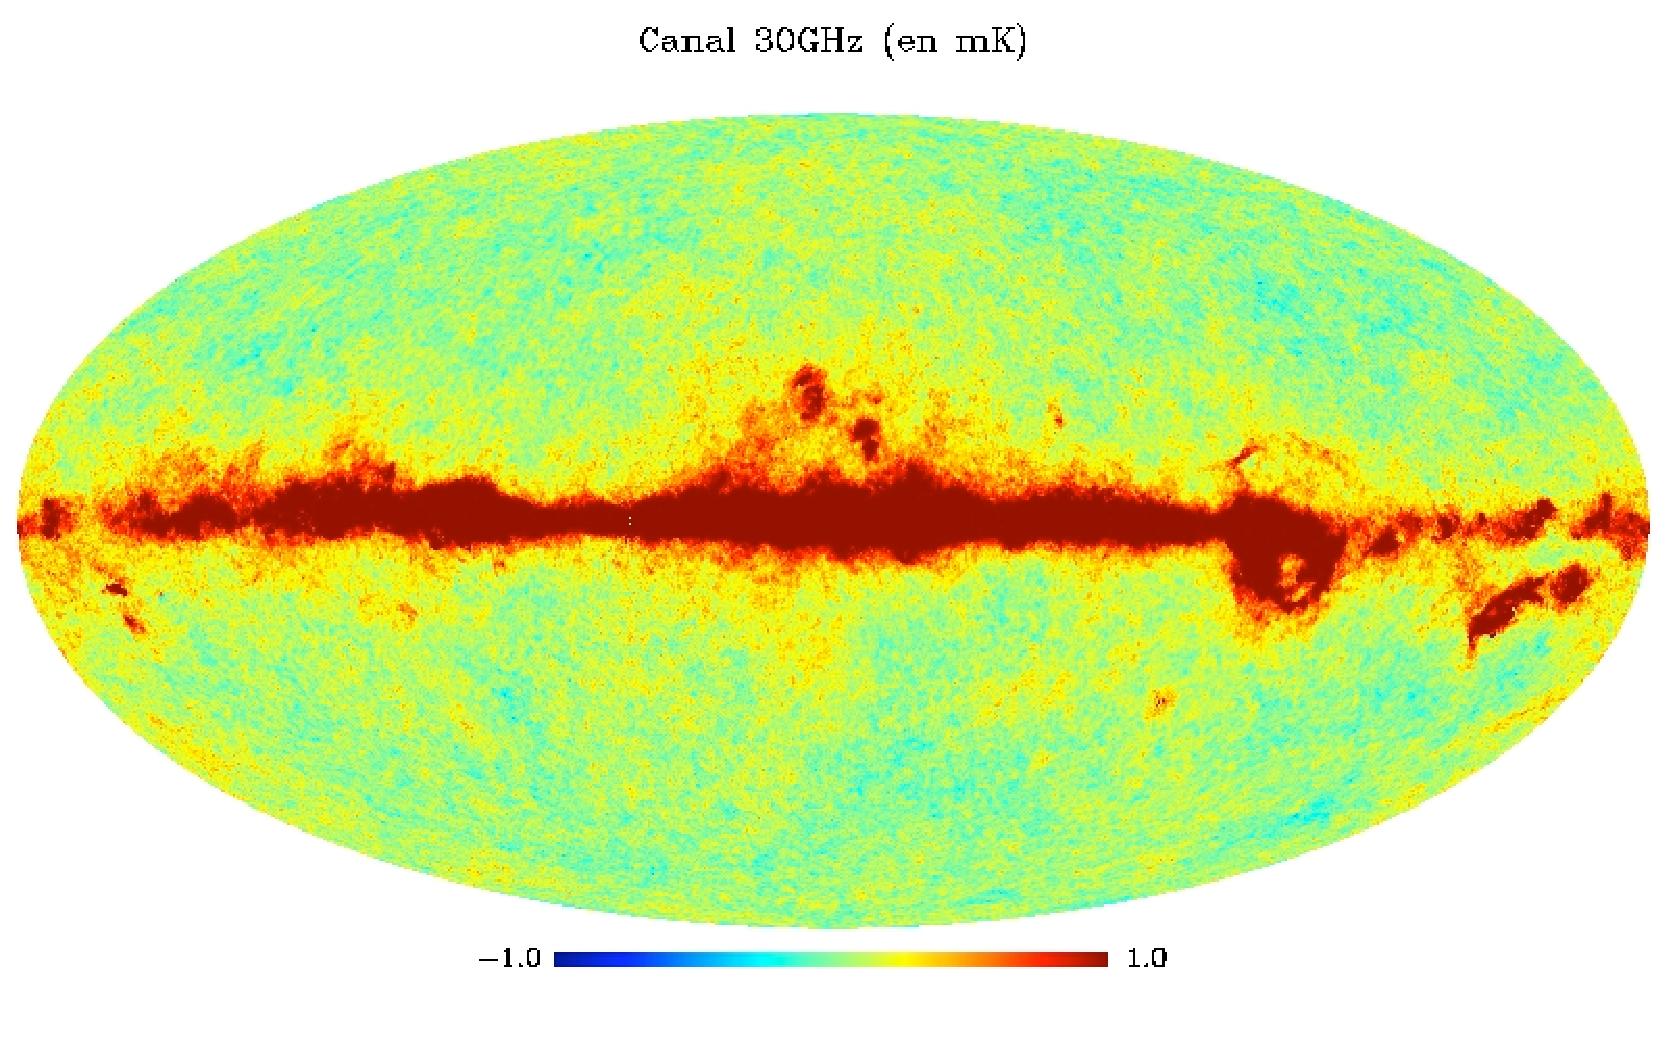
\includegraphics[width=6cm]{input30Ghz.pdf}}
\end{minipage}
\hfill
\begin{minipage}[b]{0.5\linewidth}
    \centerline{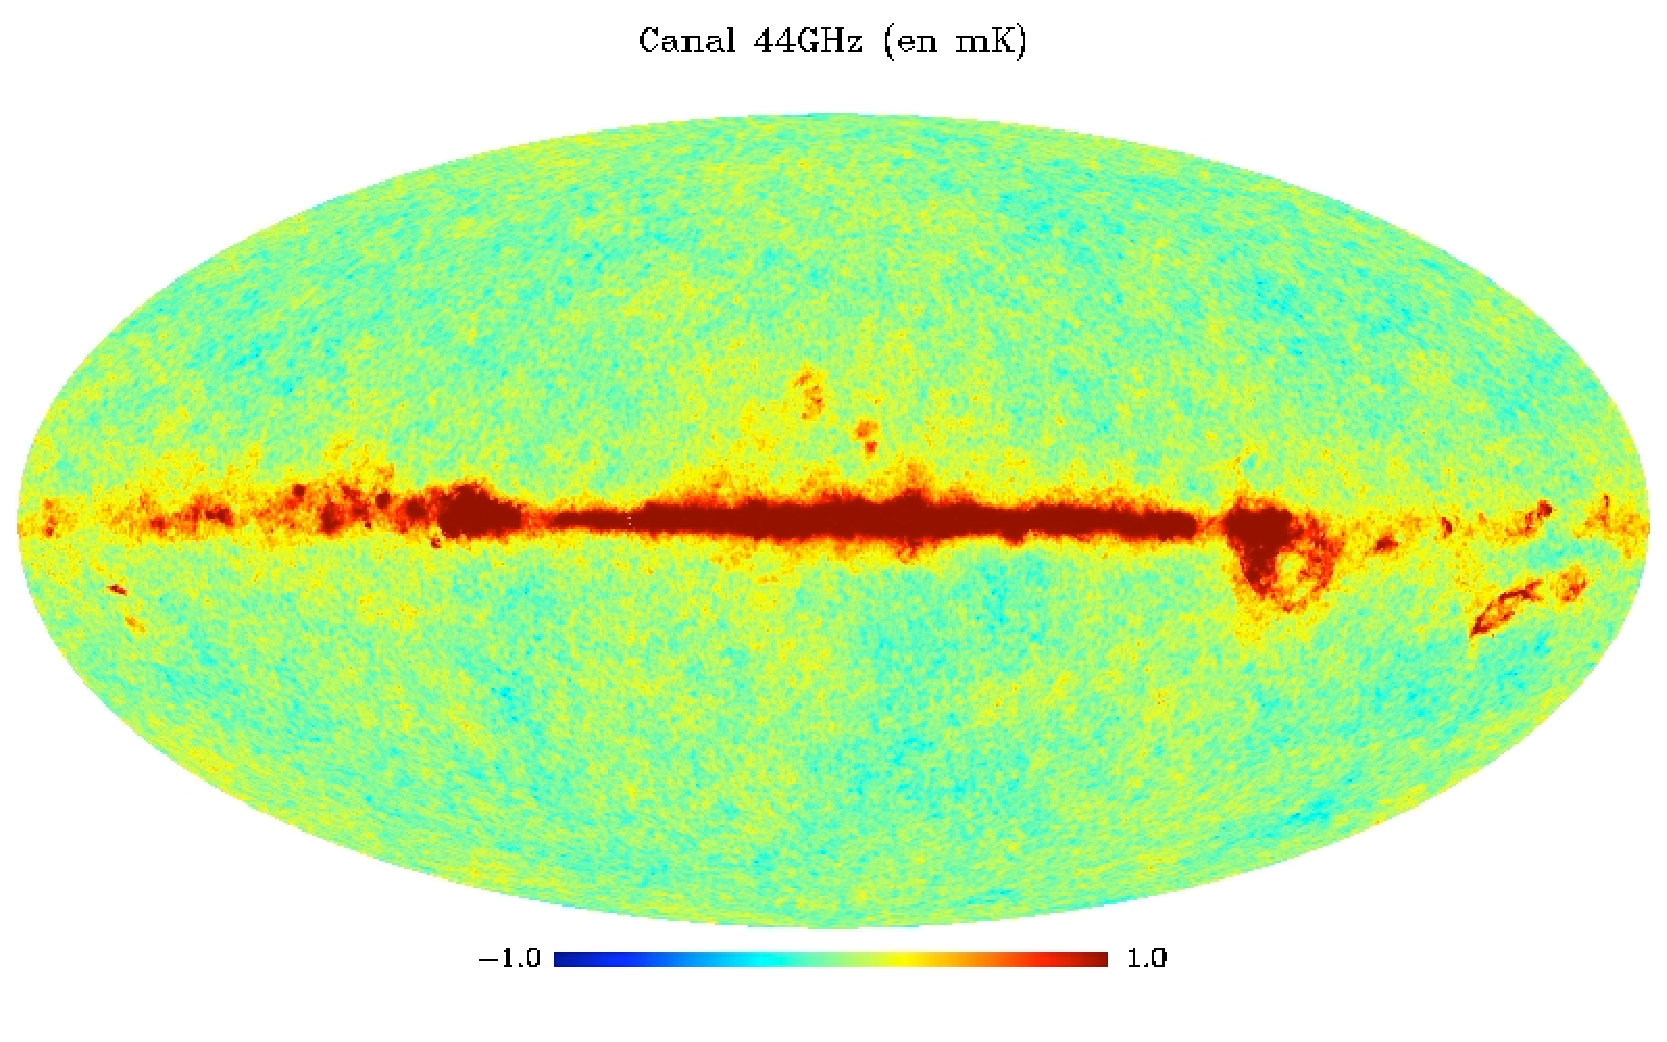
\includegraphics[width=6cm]{input44Ghz.pdf}}
\end{minipage}
\vfill
\hspace{0.1in}
\begin{minipage}[b]{0,5\linewidth}
    \centerline{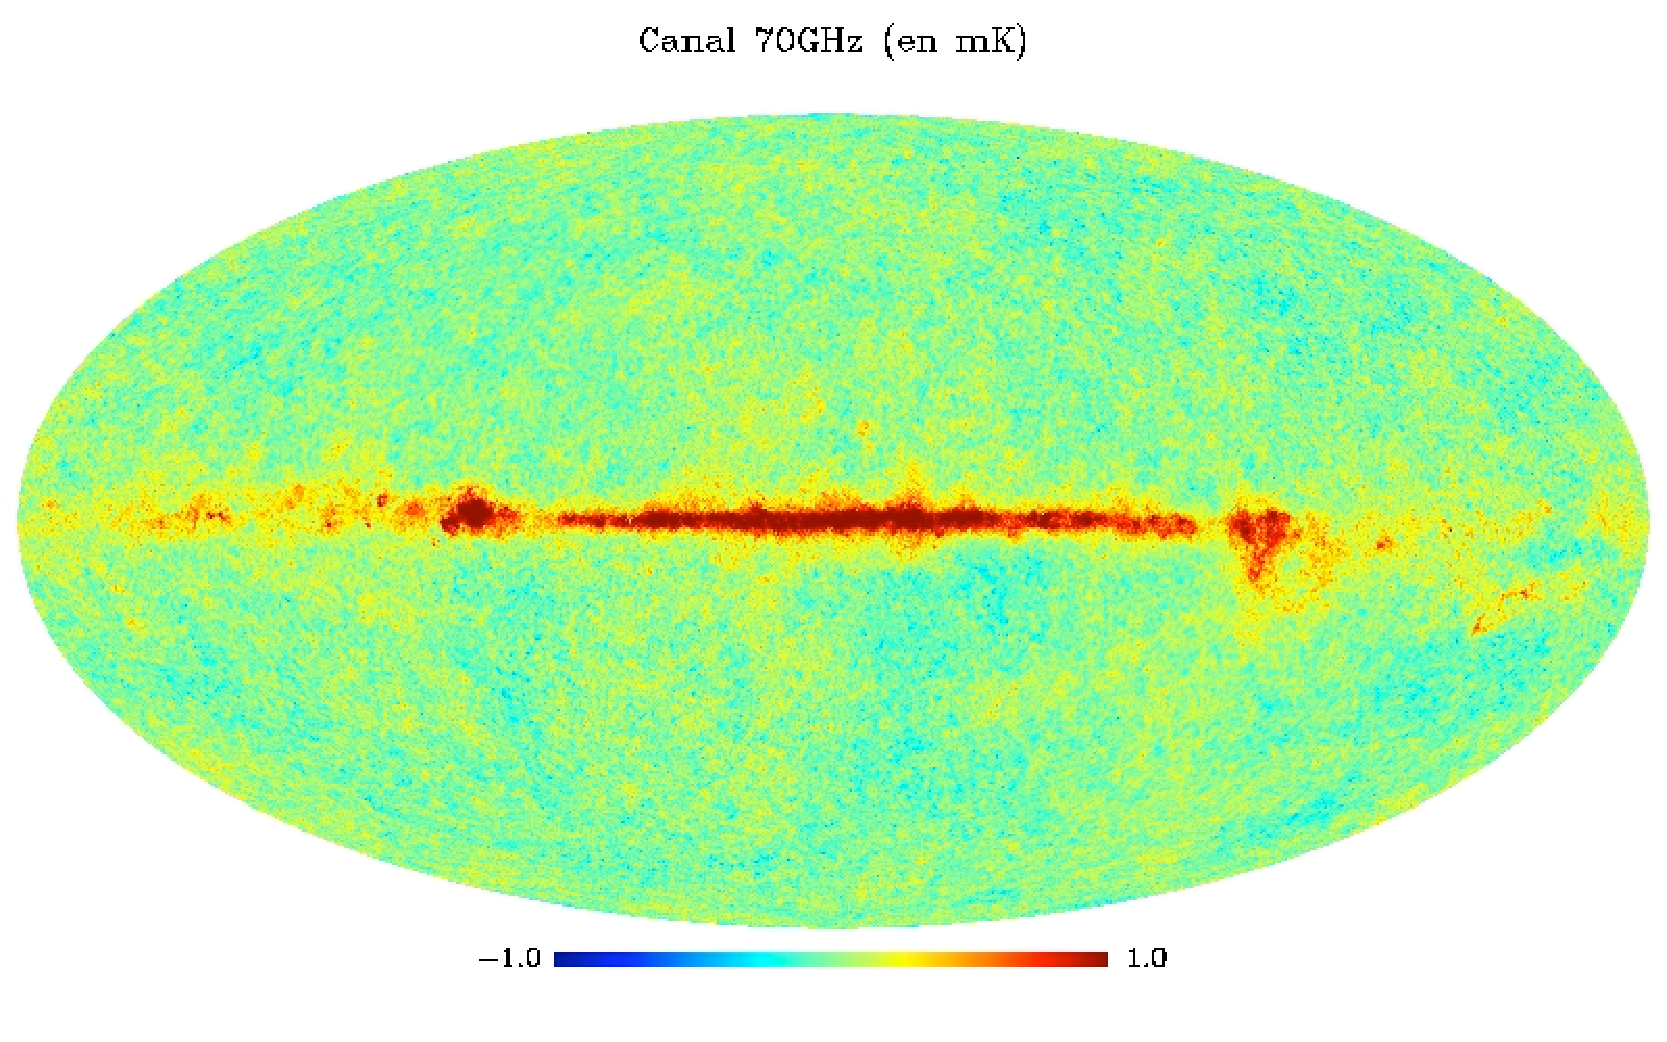
\includegraphics[width=6cm]{input70Ghz.pdf}}
\end{minipage}
\hfill
\begin{minipage}[b]{0,5\linewidth}
    \centerline{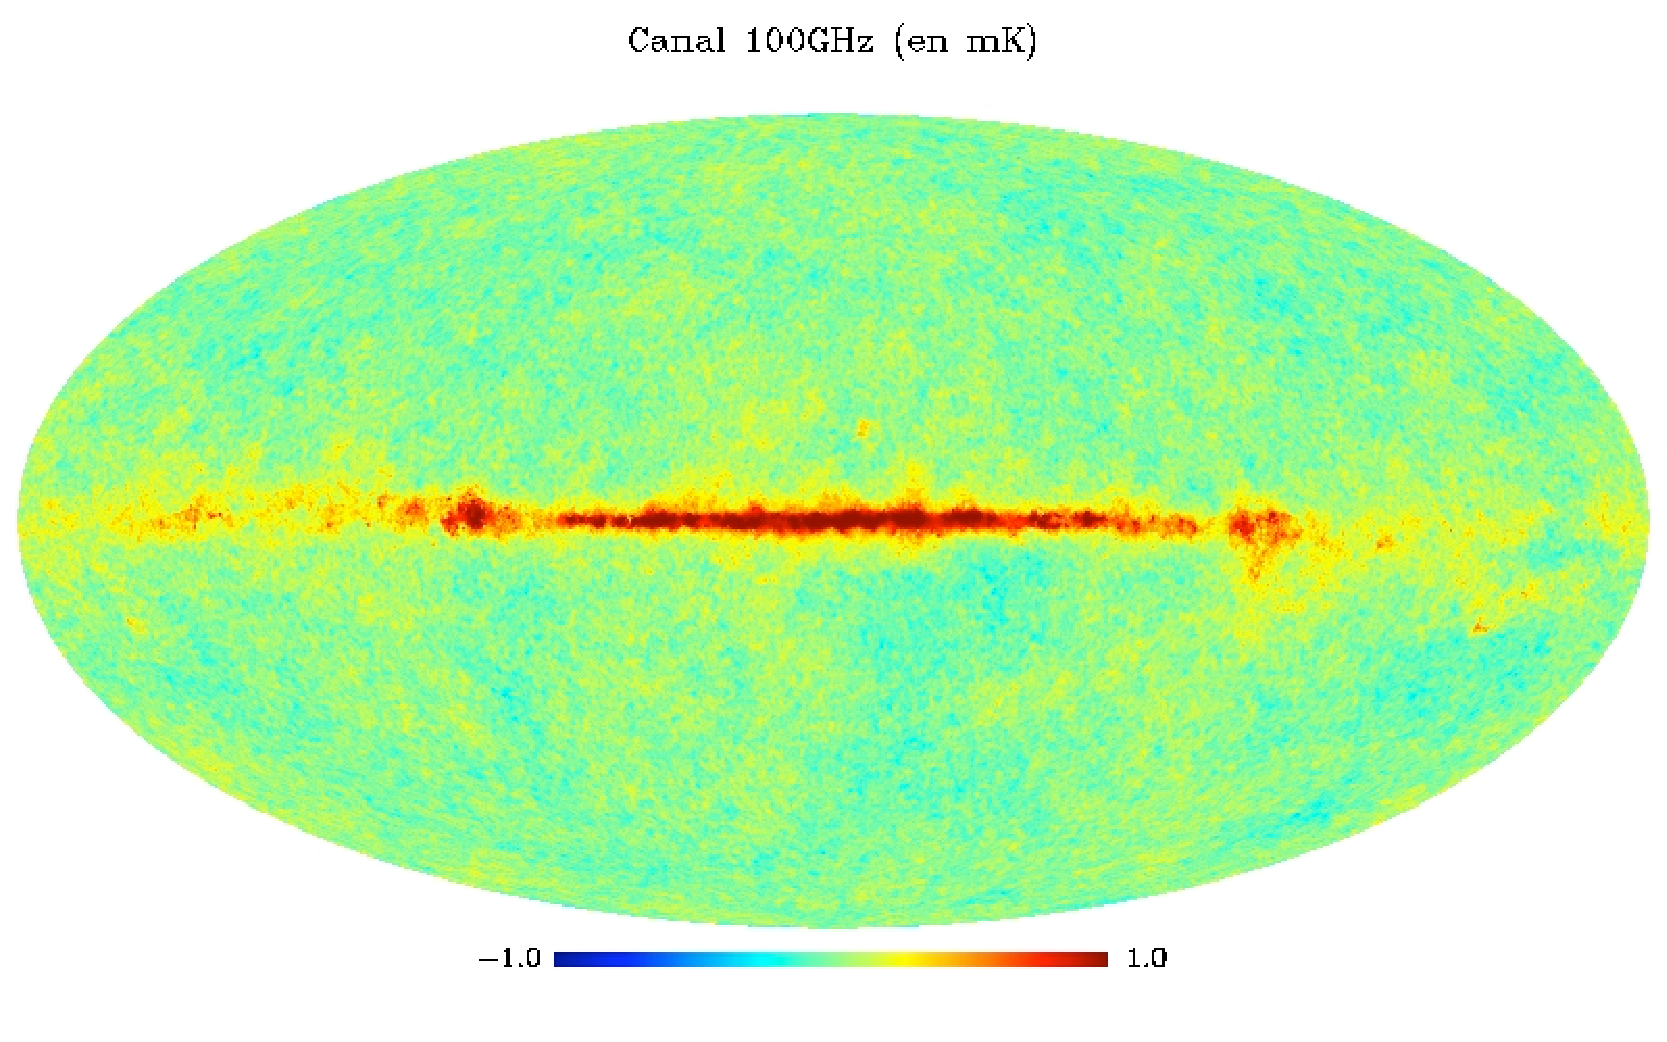
\includegraphics[width=6cm]{input100Ghz.pdf}}
\end{minipage}
\vfill
\hspace{0.1in}
\begin{minipage}[b]{0,5\linewidth}
    \centerline{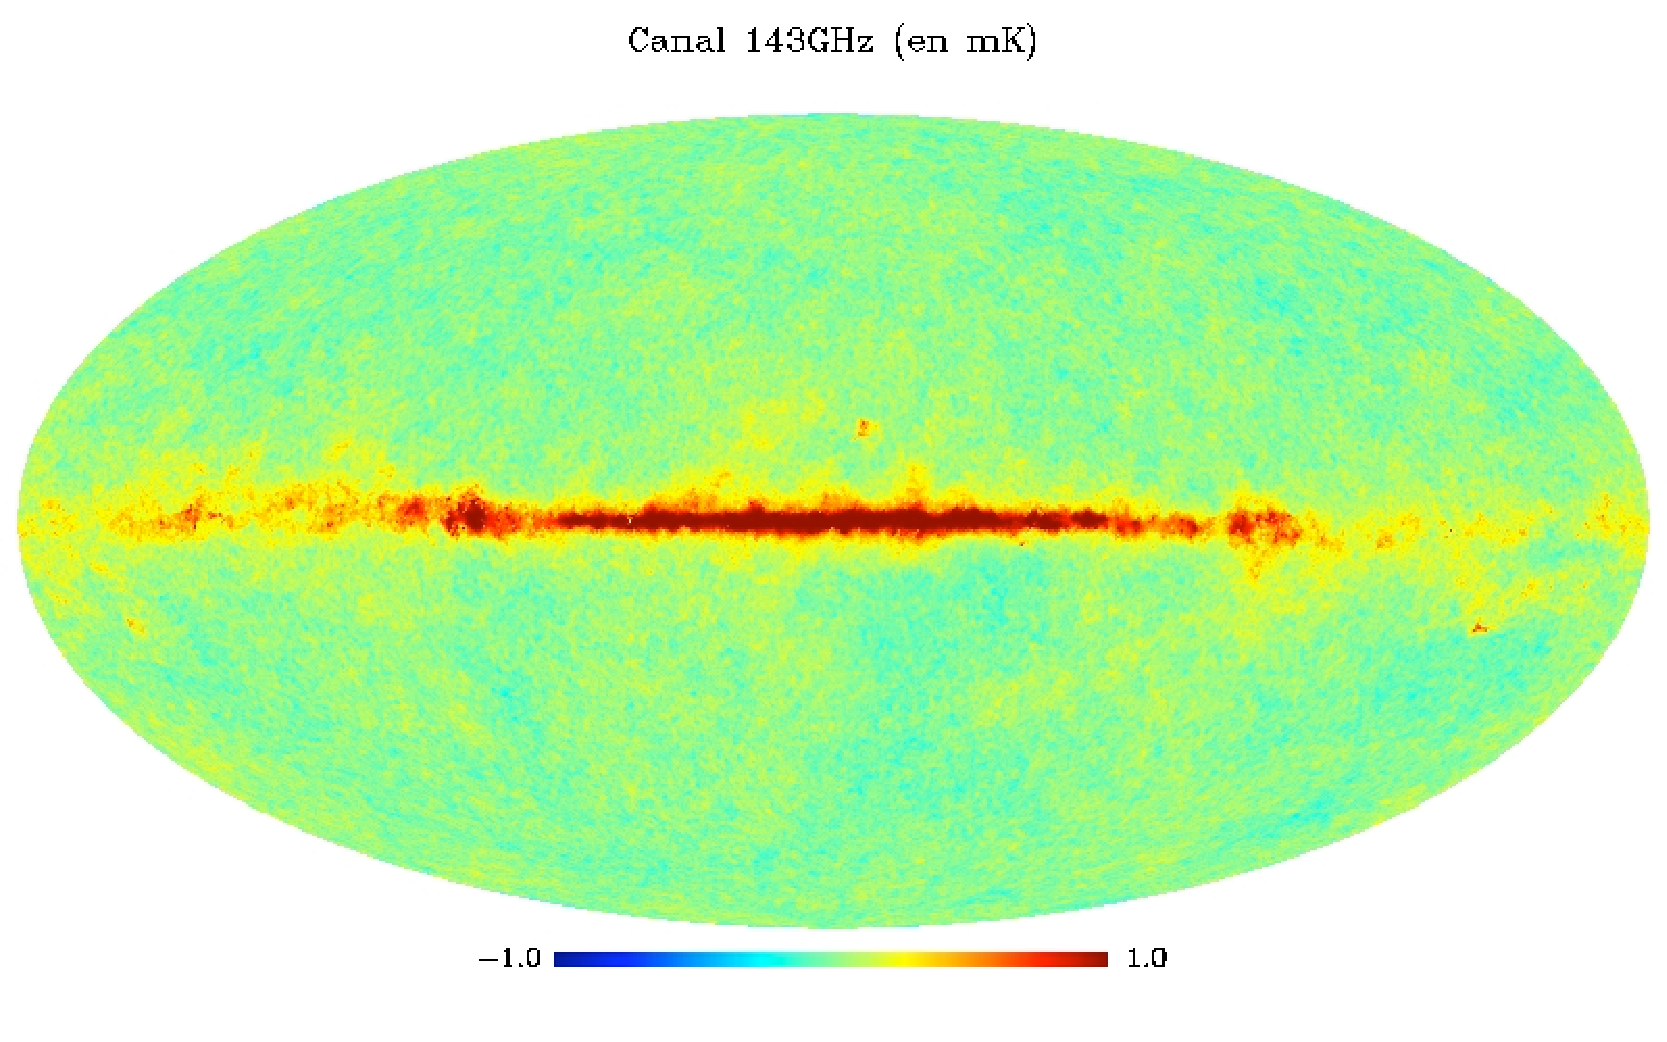
\includegraphics[width=6cm]{input143Ghz.pdf}}
\end{minipage}
\hfill
\begin{minipage}[b]{0,5\linewidth}
    \centerline{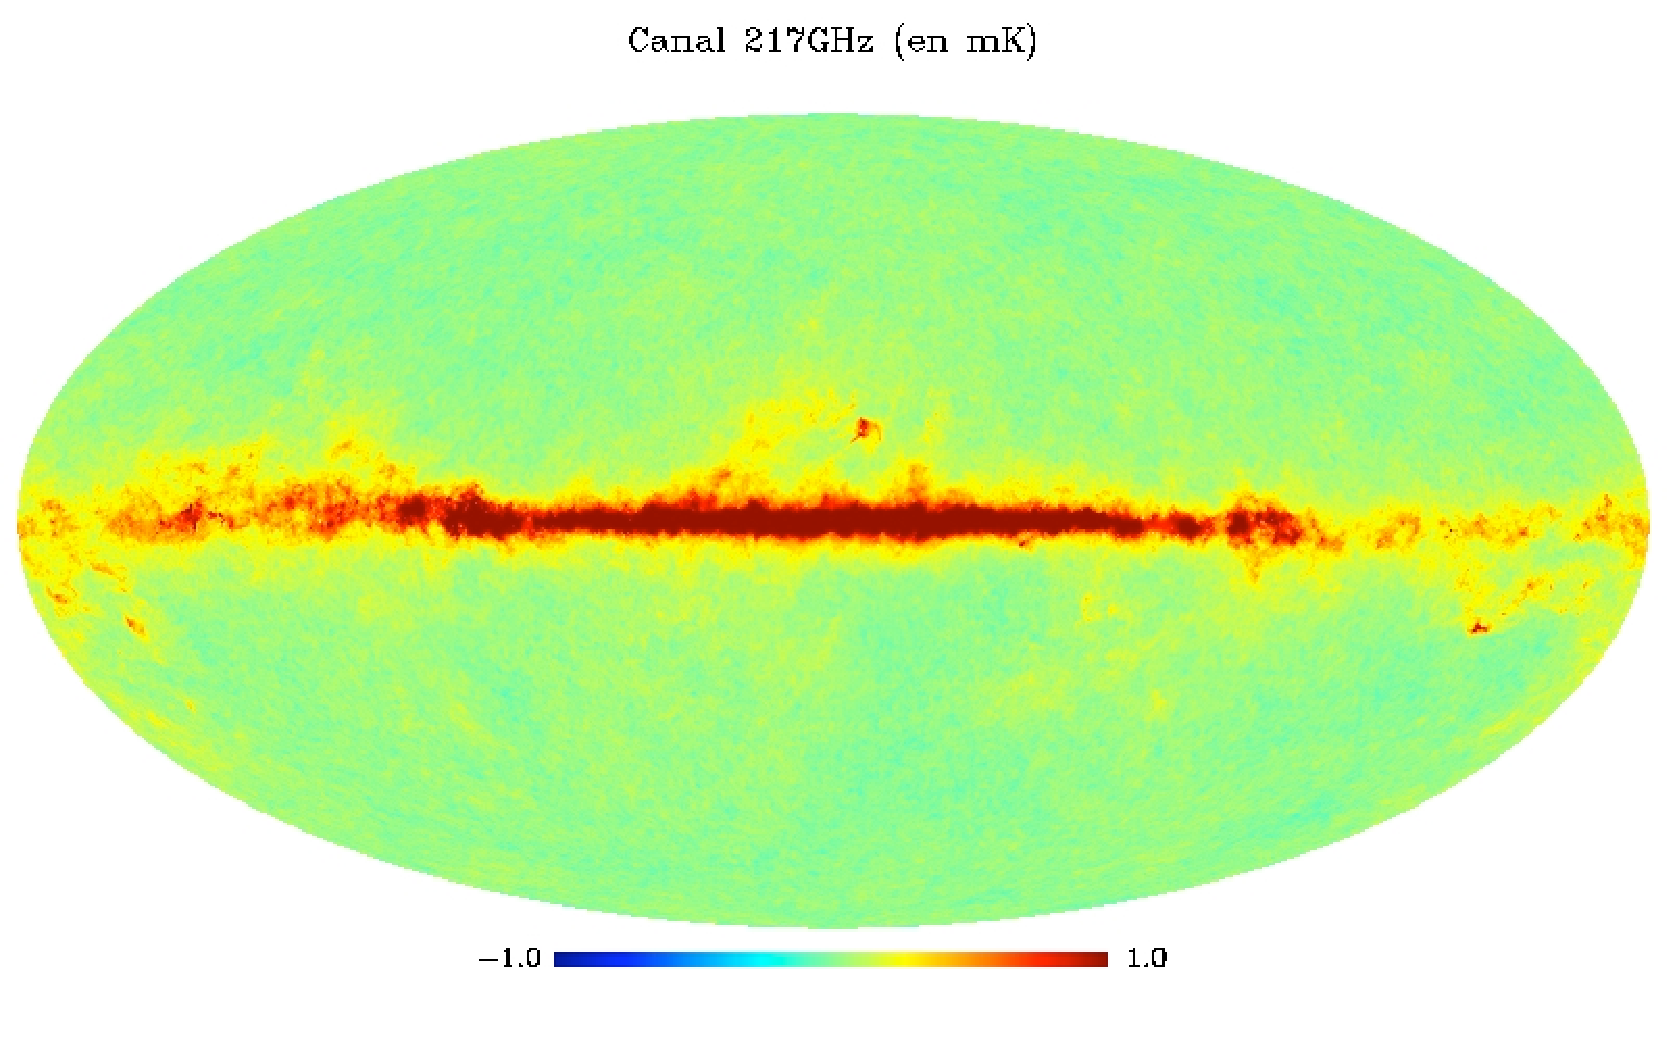
\includegraphics[width=6cm]{input217Ghz.pdf}}
\end{minipage}
\vspace{-0.1in} 
\vfill
\hspace{0.1in}
\begin{minipage}[b]{0,5\linewidth}
    \centerline{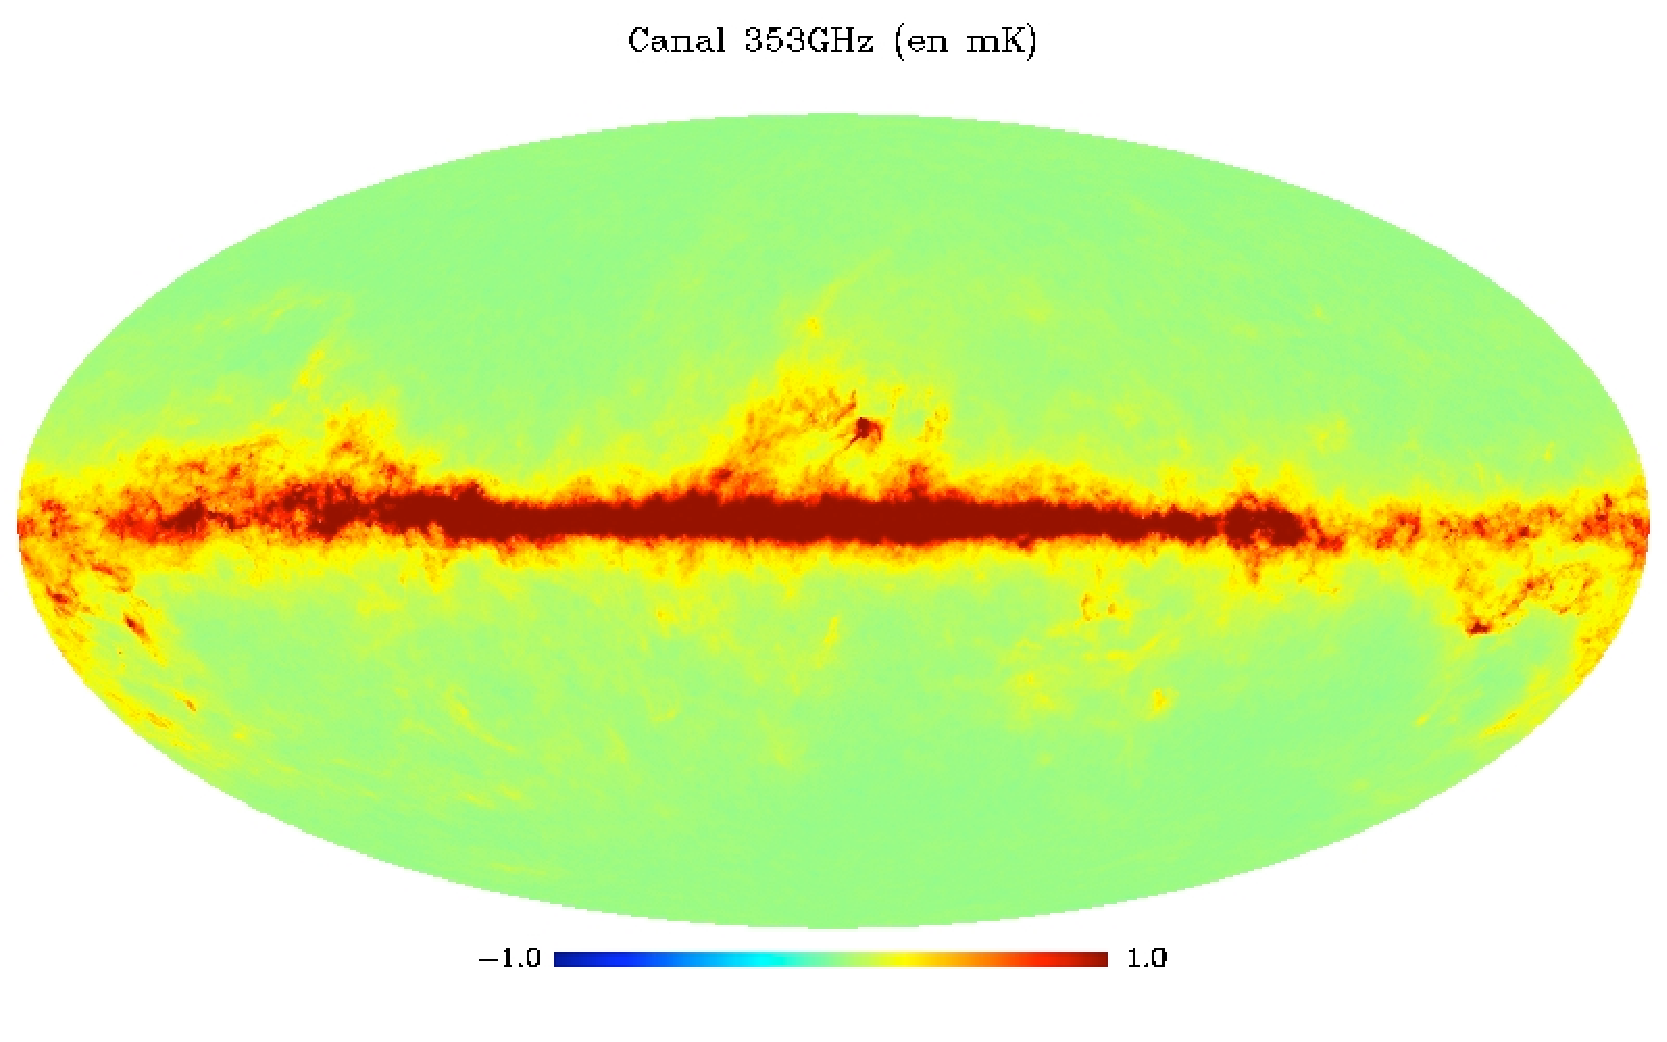
\includegraphics[width=6cm]{input353Ghz.pdf}}
\end{minipage}
\hfill
\begin{minipage}[b]{0,5\linewidth}
    \centerline{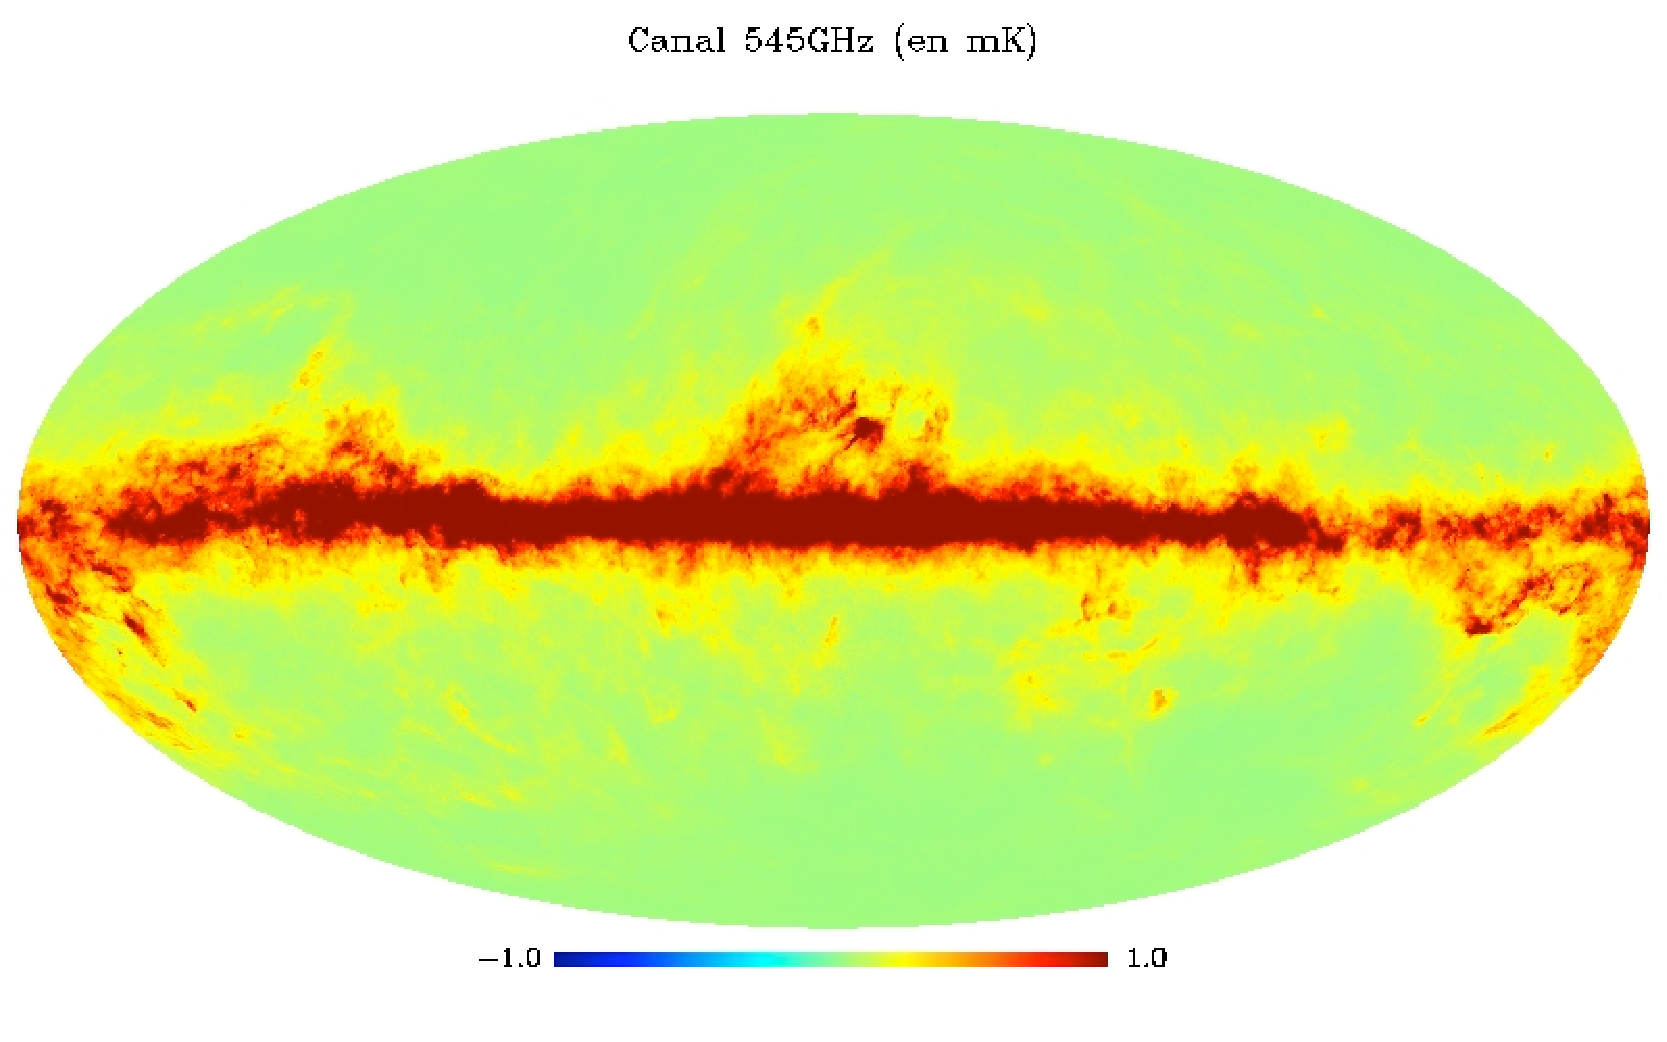
\includegraphics[width=6cm]{input545Ghz.pdf}}
\end{minipage}
\vspace{-0.1in} 
\vfill
\begin{minipage}[b]{1\linewidth}
    \centerline{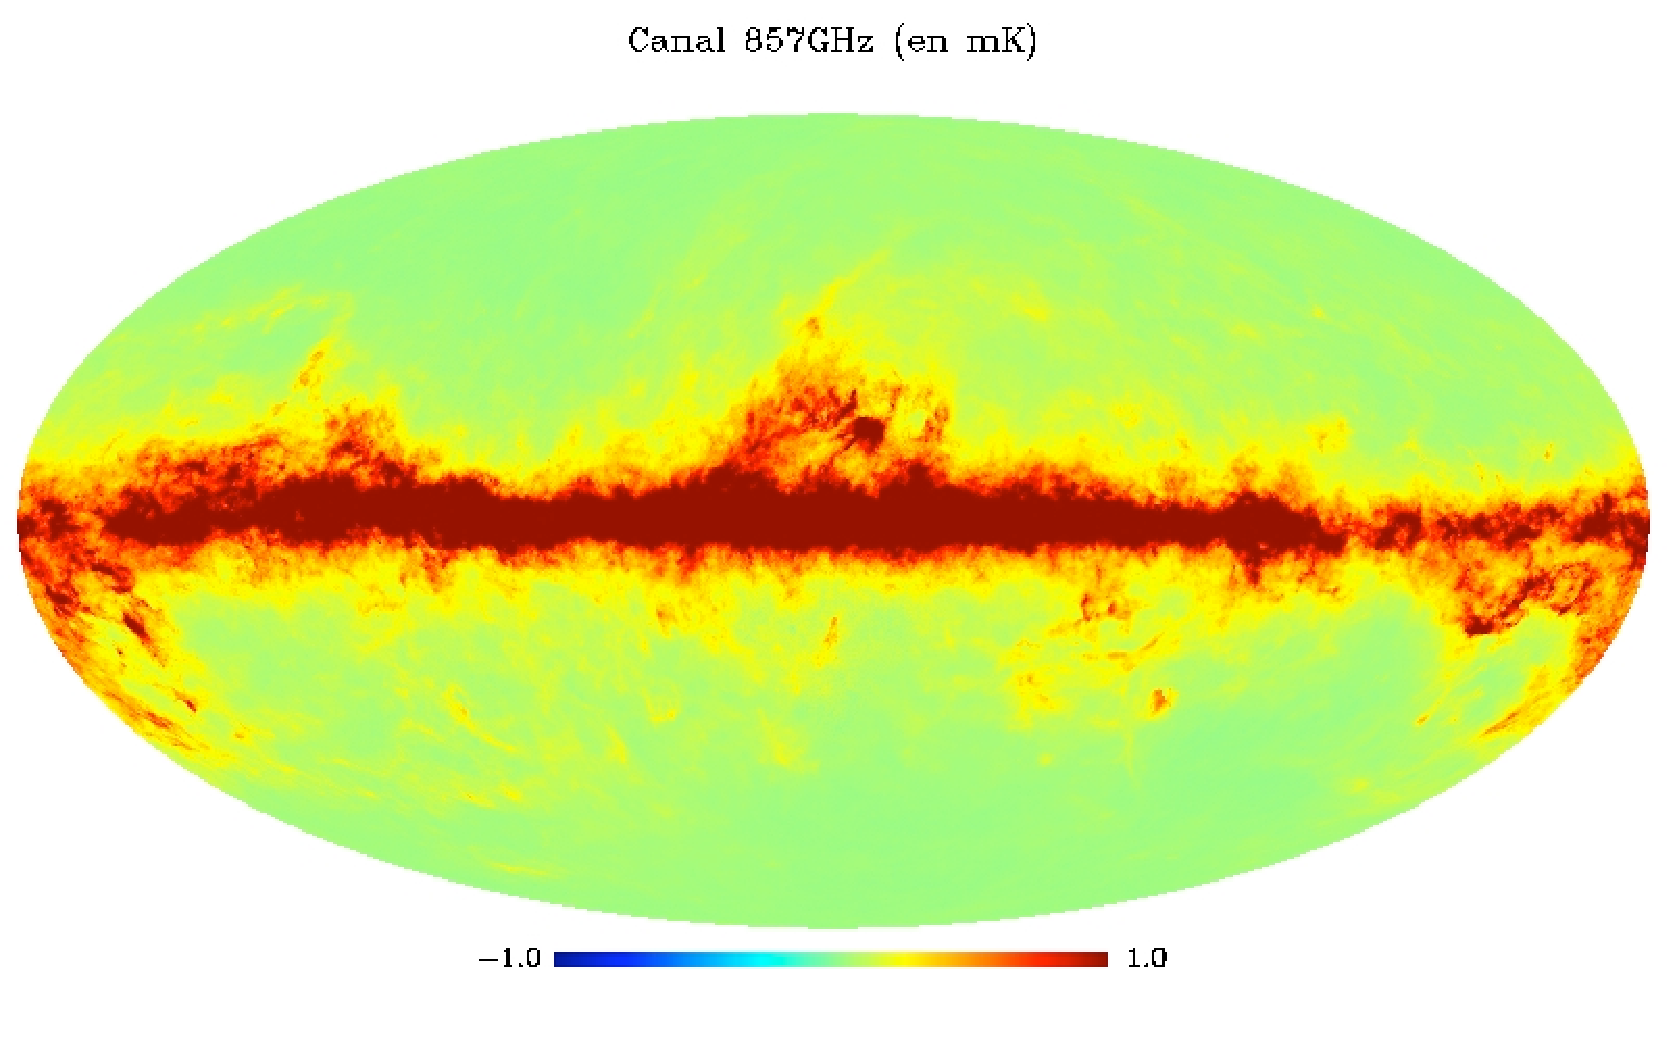
\includegraphics[width=6cm]{input857Ghz.pdf}}
\end{minipage}
\vspace{-0.1in} 

\caption{WG2/CH2 datas.}  \label{fig:data_wg2}
\end{figure}

\paragraph*{Physical model for GMCA}

Astrophysical components in the simulated datas WG2/CH2 are the folowing:\\
\begin{itemize}
\item {\bf CMB:} The only hypothesis made will be the blackbody spectrum at $2,375\,^\circ K$. The CMB column in the mixing matrix $\bf A$ will be fixed.
\item {\bf SZ:} With a point of view similar to the one used for the hypotheses on the CMB, the linear mixing model of SZ in the frequency ranges observed by Planck is checked well. 
More, the spectral behaviour of SZ is well-known. The SZ column in the mixing matrix $\bf A$ will also be considered known and so fixed.
\item {\bf "Free-Free":} In first approximation, the linear mixing model is checked for the component "Free-Free". Its spectral behaviour is the one of a power law with 
spectral index $\beta^{FF} \simeq 2,15$ \citep{Delabrouille:2005dn}.
\item {\bf "Synchrotron":} Physical models are expecting the synchrotron emissions to have a spectral behaviour like a power law with spatial evolution. The linear mixture model 
is no longer valid. In \citep{Bonaldi:2006fu} it has been proposed to approximate the synchrotron's behaviour as a linear mixture whose spectral index is to be estimated. This hypothesis 
should be accurate for the large scale structures of the synchrotron. More, in \citep{Haslam:1982dk} a synchrotron map with a resolution closed to a quarter of Planck's one have been proposed. 
Our idea is to add an estimation step in the algorithm GMCA in which the spectral index $\beta^{sync}$ will be estimated with a residual cube ${\bf R} = {\bf X} - \sum_{i \neq sync} {\bf a}^i {\bf s}_i$ 
and with the low resolution synchrotron map ${\bf s}_{Haslam}$. $\beta^{sync}$ estimation is done with signals with same resolution (the Haslam map's one) in the following way:
\begin{equation}
\beta^{sync} = \Argmin{\beta} \left\|{\bf R} - {\bf a}^{sync}\left(\beta\right) {\bf s}_{Haslam} \right\|_F
\end{equation}
\item {\bf "Dust":} Thermal dust component is a non-linear mixture. This is the most complex component to modelize since she requires two set of parameters (temperature and spectral index), 
both having spatial variations. Fortunatly, CMB and dust have opposite spectral behaviour: CMB is dominant in low frequency channels whereas dust dominates in high frequency channels. Moreover, 
dust component is highly structured with a sparse decomposition in wavelets. GMCA being built to be sensible to that kind of component, it seems acceptable to recover the dust component 
(or perhaps we should speak of components) blindly.
\item {\bf Point sources:} Infra-red or radio point sources each have their own spectrum. They are more an annoying component towards the goal of extracting diffuses components like CMB. 
Their detection is one of the troubles discovered during the processing of the datas (see~\citep{leach08}). After their detection they are often masked.
\end{itemize}

\paragraph*{GMCA algorithm for Planck}

The linearity of BSS model has a major advantage as soon as physical parameters' estimation is needed: for example, once you know the noise's statistical properties on the datas, 
the linearity of the model allows to get the noise's statistical properties of the sources in an easy way.The GMCA's version described here considers WG2/CH2 datas as a linear 
mixture of components. Beyond the algorithms \ref{algo_gmca} and \ref{algo_fast_gmca} already described, GMCA method is itself ready to include the physical constraints described above.

For the linear mixture model, each observation $\{{\bf x}_i\}_{i=1,\cdots,m}$ could be written as the linear combination of $n$ components. The observed datas, including convolution, 
are thus defined in the following way:
\begin{eqnarray}
\forall i=1,\cdots,m; \quad {\bf y}_i &  = & ({\bf h}_i \star {\bf x}_i) + {\bf n}_i \\
& = &  \sum_{j=1}^n A[i,j] ({\bf h}_i \star {\bf s}_j) + {\bf n}_i
\end{eqnarray}
The mixture model is no longer linear towards the observed datas $\bf Y$\footnote{It is a non linearity in the sense of the mixing model, the model remains linear in common sense since it is defined as the composition of linear operators.}. Two solutions could be considered: a strict one will the deconvolution of each observation before applying GMCA.
\begin{itemize}
\item {\bf Deconvolution of the datas:} A deconvolution is done to each observation. The datas having an interchannel structure, a separate deconvolution of each channel is unsuitable. 
Regardless of these considerations, some convolution kernels (especially for low frequecy channels) are leading to an ill-conditioned deconvolution.
\item {\bf Adapt GMCA to joint deconvolution:} GMCA algorithm relies on the iterative estimation of sources and mixing matrix. A deconvolution could be intergrated to 
the sources estimation step for fixed $\bf A$.
\end{itemize}
Due to the really huge size of the datas, we have first chosen to apply GMCA to the datas $\bf Y$. A compensation of the convolution is then done on the estimated CMB map. In first approximation, 
the most significant diffused structures in the datas are dominated by their lowest frequencies for which the convolution operator has the less impact. This point allows us to justify the estimation 
of the mixing matrix $\bf A$ from the datas $\bf Y$.

The GMCA method adapted for the processing of Planck datas is described in Algorithm~\ref{algo_planck_gmca}.
{\linespread{1}
\begin{algorithm}[htb]
\caption{Planck GMCA algorithm.}
\label{algo_planck_gmca}
\noindent{\bf Task:} Separation of Planck datas with GMCA.\\
\noindent{\bf Parameters:} The data $\bf Y$, number of iterations $P_{\max}$, number of sources $N_s$ and channels $N_c$, dictionnary ${\bf \Phi}$, 
mixing matrix $\bf A$ with fixed column setted, initial threshold $\gamma^{(0)}$ stopping threshold ${\gamma_{\min}}$.\\
\noindent{\bf Initialization:} 
\begin{itemize}
\item Set set number of iterations $P_{\max}$ and the initial threshold $\gamma^{(0)}$.
\item Computes a wavelet transform on the sphere of the datas ${\bf \balpha_Y}$.\\
${\bf \balpha_Y} = {\bf Y} {\bf \Phi}^T$
\end{itemize}
\noindent{\bf Main iteration:} \\
\While{ Threshold $\gamma^{(h)} > \gamma_{\min}$ (\textit{e.g.} depends on the noise variance)}{
\begin{itemize}
\item Estimation of the sources ${\bf \balpha_S}$ at iteration $h$ with matrix $\bf A$ supposed fixed:\\
${\bf \balpha_{S}}^{(h+1)} = \mathcal{H}_{\gamma^{(h)}}\left({\bf A^\dagger}^{(h)}{\bf \balpha_Y}\right)$
\item Update the free column of the mixing matrix $\bf A$ noted ${\bf A^\circ}$ with ${\bf \balpha_S}$ supposed fixed:\\
${\bf \tilde{A^\circ}}^{(h+1)} = {\bf \balpha_Y}{\bf \tilde{\balpha^\circ}_S}^{{(h)}^T} \left({\bf \tilde{\balpha^\circ}_S}^{{(h)}}{\bf \tilde{\balpha^\circ}_S}^{{(h)}^T}\right)^{-1}$
\item Estimation of synchrotron's spectral index $\beta^{sync}$ from the residual ${\bf \balpha_R} = {\bf \balpha_Y} - \sum_{i \neq sync} {\bf a}^i {\bf \balpha_{S}}_i$:\\
$\beta^{sync} = \Argmin{\beta} \left \| {\bf \balpha_R} - {\bf a}^{sync} {\bf \balpha}_{Haslam} \right \|_2$
\item Update the synchrotron column of $\bf A$
\item Decrease the threshold $\gamma^{(h)}$.
\end{itemize}
}
\noindent{\bf Output:} Estimated mixing matrix ${\bf \tilde{A}}^{(\niter)}$.
\end{algorithm}}

\subsubsection{Results}

Most of the results are for the estimation of the CMB map. The figure~\ref{fig:wg2_maps} gives the initial simulated CMB map (top) and the one estimated with GMCA (bottom). 
A remark is that GMCA estimates a miximg matrix $\bf A$ used to estimate a noisy CMB map by applying the pseudo-invert of $\bf A$ to the datas $\bf Y$. In the hypothesis of 
a perfect separation of the components, the estimated CMB map is isotropic and so characterized only by its power spectrum. Convolution of the datas lead to a power loss that 
could be corrected by the computation of a filter determined with the convolutions' kernels $\{{\bf h}_i\}_{i=1,\cdots,m}$ and the mixing matrix $\bf A$. The denoising of 
the CMB map is then done with a Wiener filtering in the spherical harmonics space. The map estimated by GMCA in figure~\ref{fig:wg2_maps} is this map obtained after Wiener filtering. 
It is well known that Wiener filtering induces a biais all the more important so SNR is low. In first approximation, the noise's spectrum is flat (stationnary in spherical harmonics space). 
The spatial spectrum of the CMB has a decreasing in the range of $1/\ell$, thus the biais on the filtered component will be greater for high $\ell$ values. This explains the differences 
between the original map and the estimated CMB map which shows a loss in high frequency structures (high $\ell$ values) on the estimated map.

In order to precisely analyse the estimated map, a solution is to observe the residual ${\bf r}_{CMB} = {\bf s}_{CMB} - {\bf \tilde{s}}_{CMB}$ (between the input map and the estimated map) 
convolved by a gaussian beam, which allows the a more suitable estimation of large structures (low $\ell$ values). Here we make comparisons between the map estimated with GMCA and maps 
estimated by the groups ADAMIS, CCA and MEM whose methods could be found in \citep{leach08}. The residual convolved with a gaussian kernel of $20$ arcminutes (which corresponds to a 
half-height width of $\ell = 500$) are given in figures~\ref{fig:wg2_resi20} and \ref{fig:wg2_resi20_2}. At first sight, the high latitudes residual (out of galactic center) seems limited 
compared to the other results. Galactic center mainly shows a residual of galactic dust. Figures~\ref{fig:wg2_resi60} and \ref{fig:wg2_resi60_2} are the same residuals but convolved this time 
with a gaussian kernel of $60$ arcminutes (which corresponds to a half-height width of $\ell = 180$). The observation of this convolved residual mainly show the really large structures. 
It corroborates the the observations made from the residual convolved at $20$ arcminutes: GMCA with physical constraints is able to recover a CMB component whose large scales are preserved 
out of the galactic center.

Figure~\ref{fig:wg2_resiperlat} shows the standard deviation of the residual convolved at $20$ (top) and $60$ (bottom) per latitude bands with a width of $20^\circ$. The value $90^\circ$ corresponds 
to the galactic center and since this band is highly corrupted by galactical components, the corresponding result is not plotted. The bottom plot for the residual convolved at $60$ arcminutes seems to 
corroborate the good results of GMCA outside the galactic center. Strangely the result is slightly different for the residual convolved at $20$ arcminutes scince it shows a lower residual for ADAMIS. 
It seems that this is due to a diredt compensation of deconvolution. This latter one leads to create \textit{ringing} artefact araound residual structures of point sources or galactical components.

\begin{center}
\begin{figure}[htb]
$$
\begin{array}{cc}
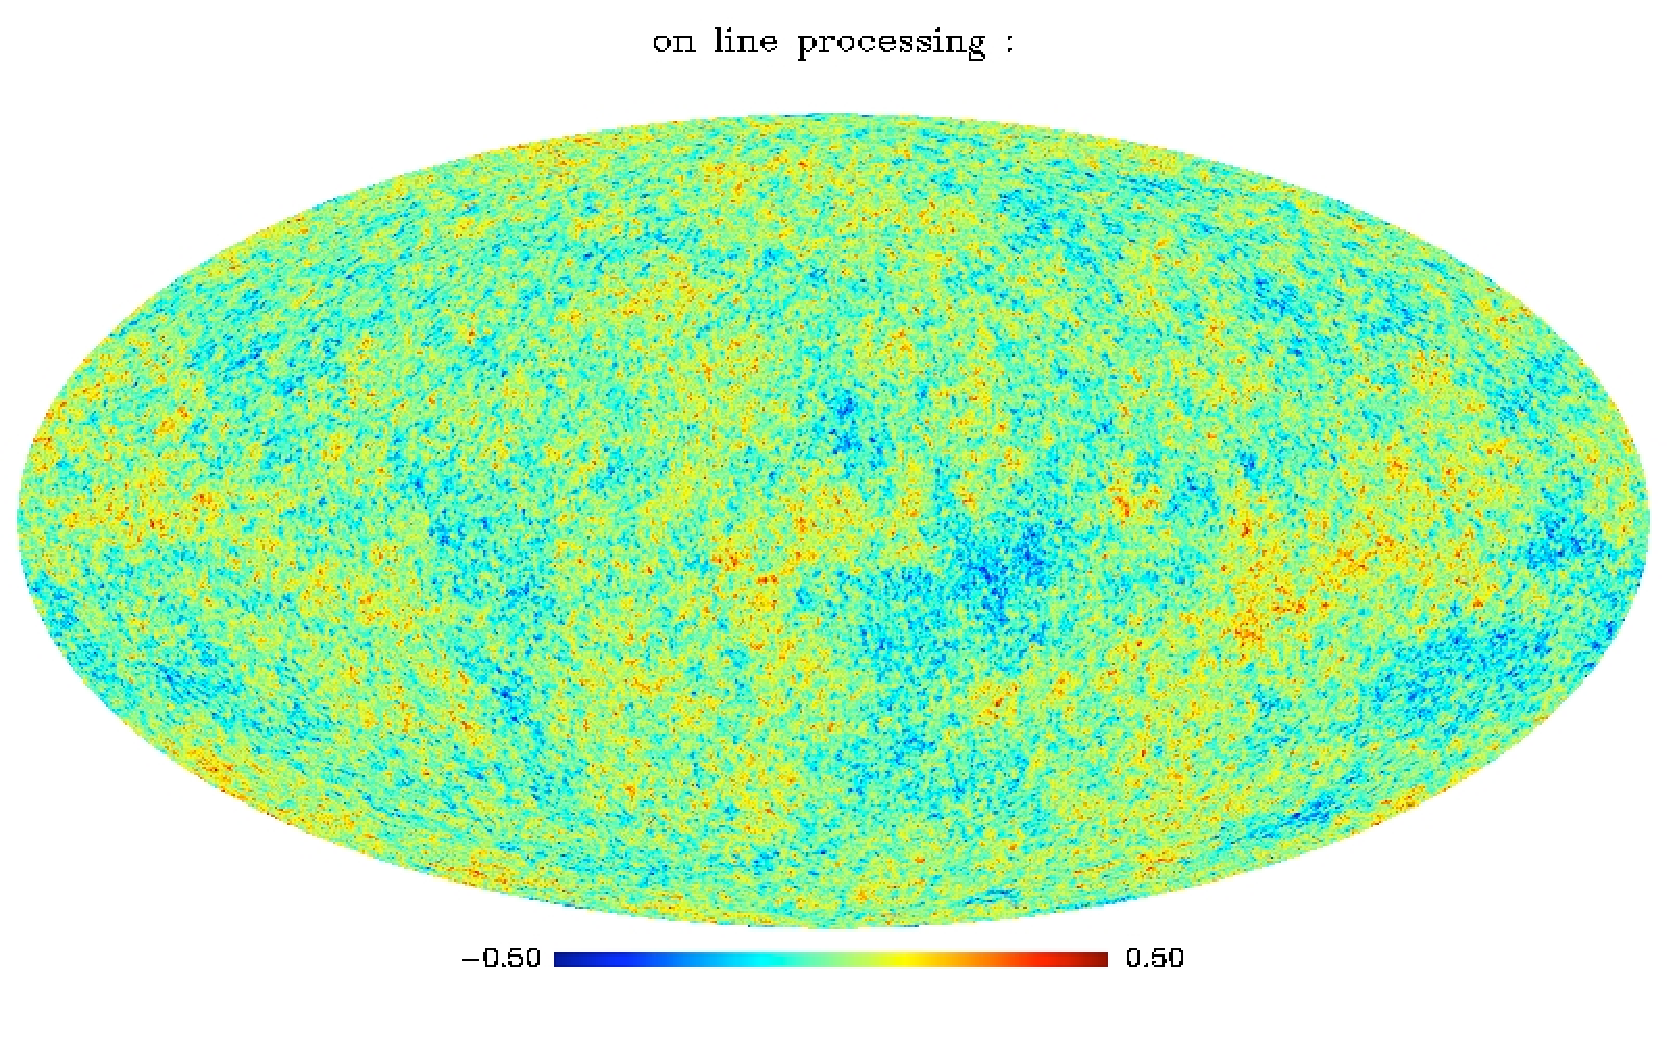
\includegraphics[width=12cm]{cmb_input.pdf} \\
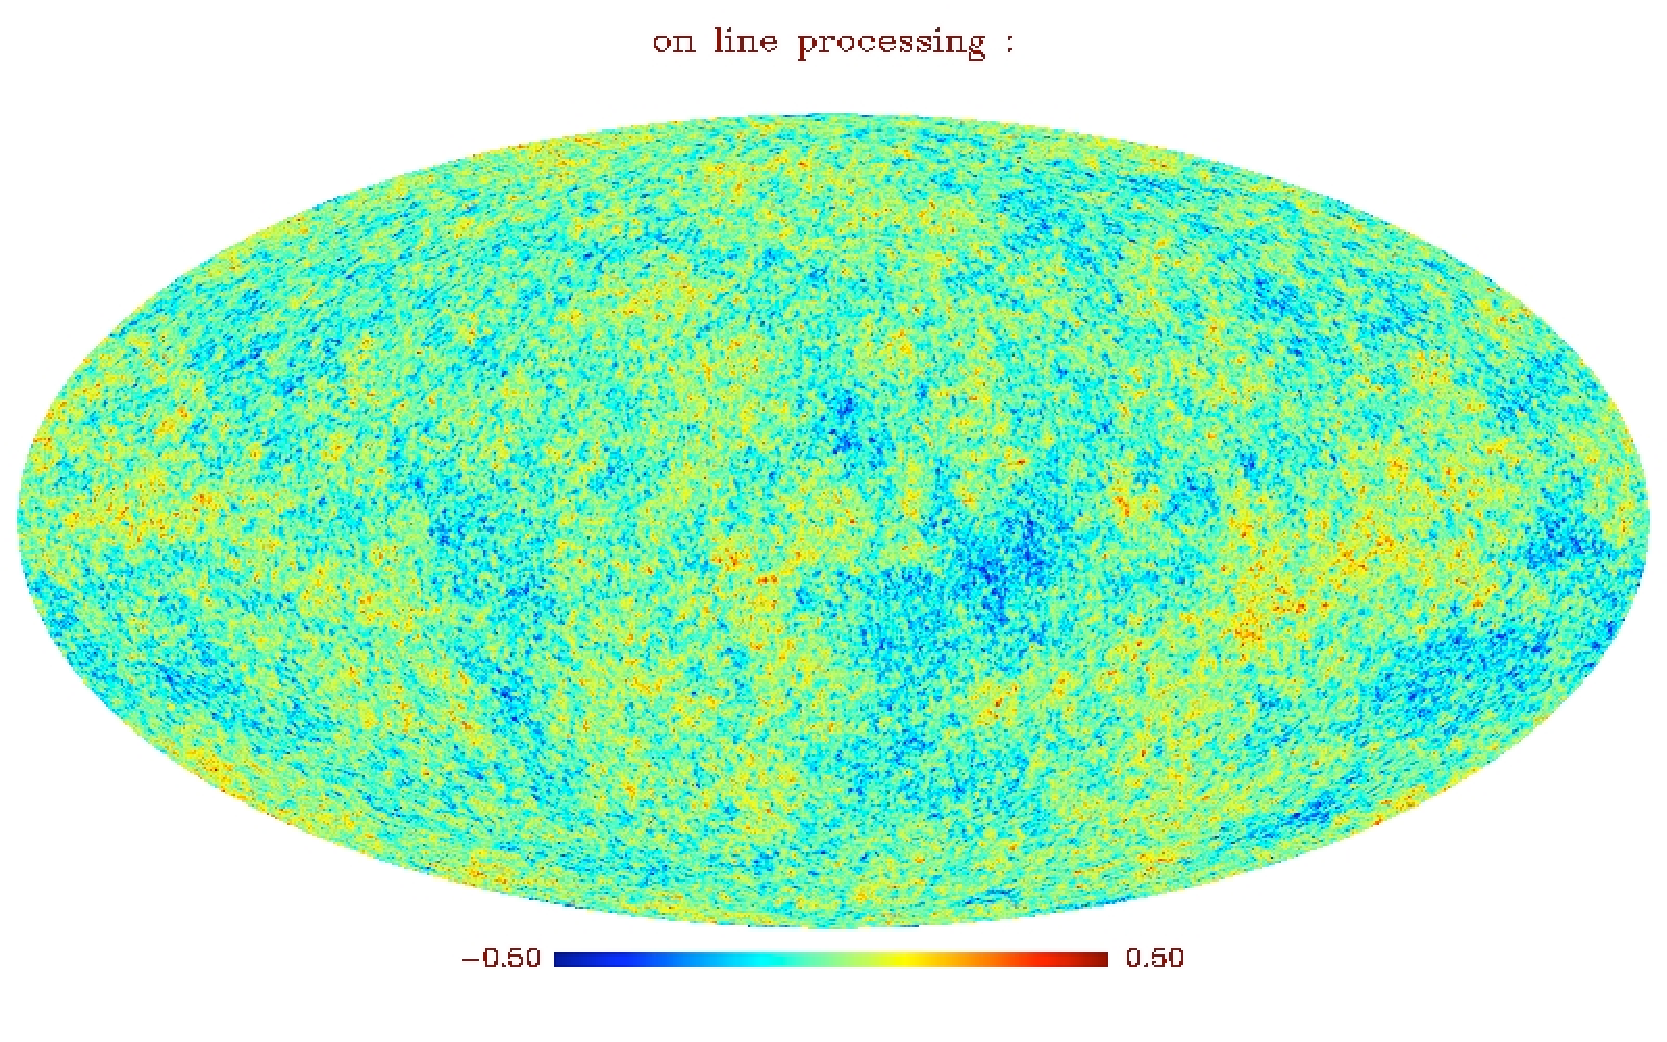
\includegraphics[width=12cm]{gmca_cmbwiener.pdf}
\end{array}
$$
\vspace{-0.1in} \caption{\textbf{Top~:} original CMB component. \textbf{Bottom~:} CMB componentestimated with GMCA. \textbf{Unit~:}  $10^{-3}$K.} \label{fig:wg2_maps}
\end{figure}
\end{center}

\begin{center}
\begin{figure}[htb]
$$
\begin{array}{cc}
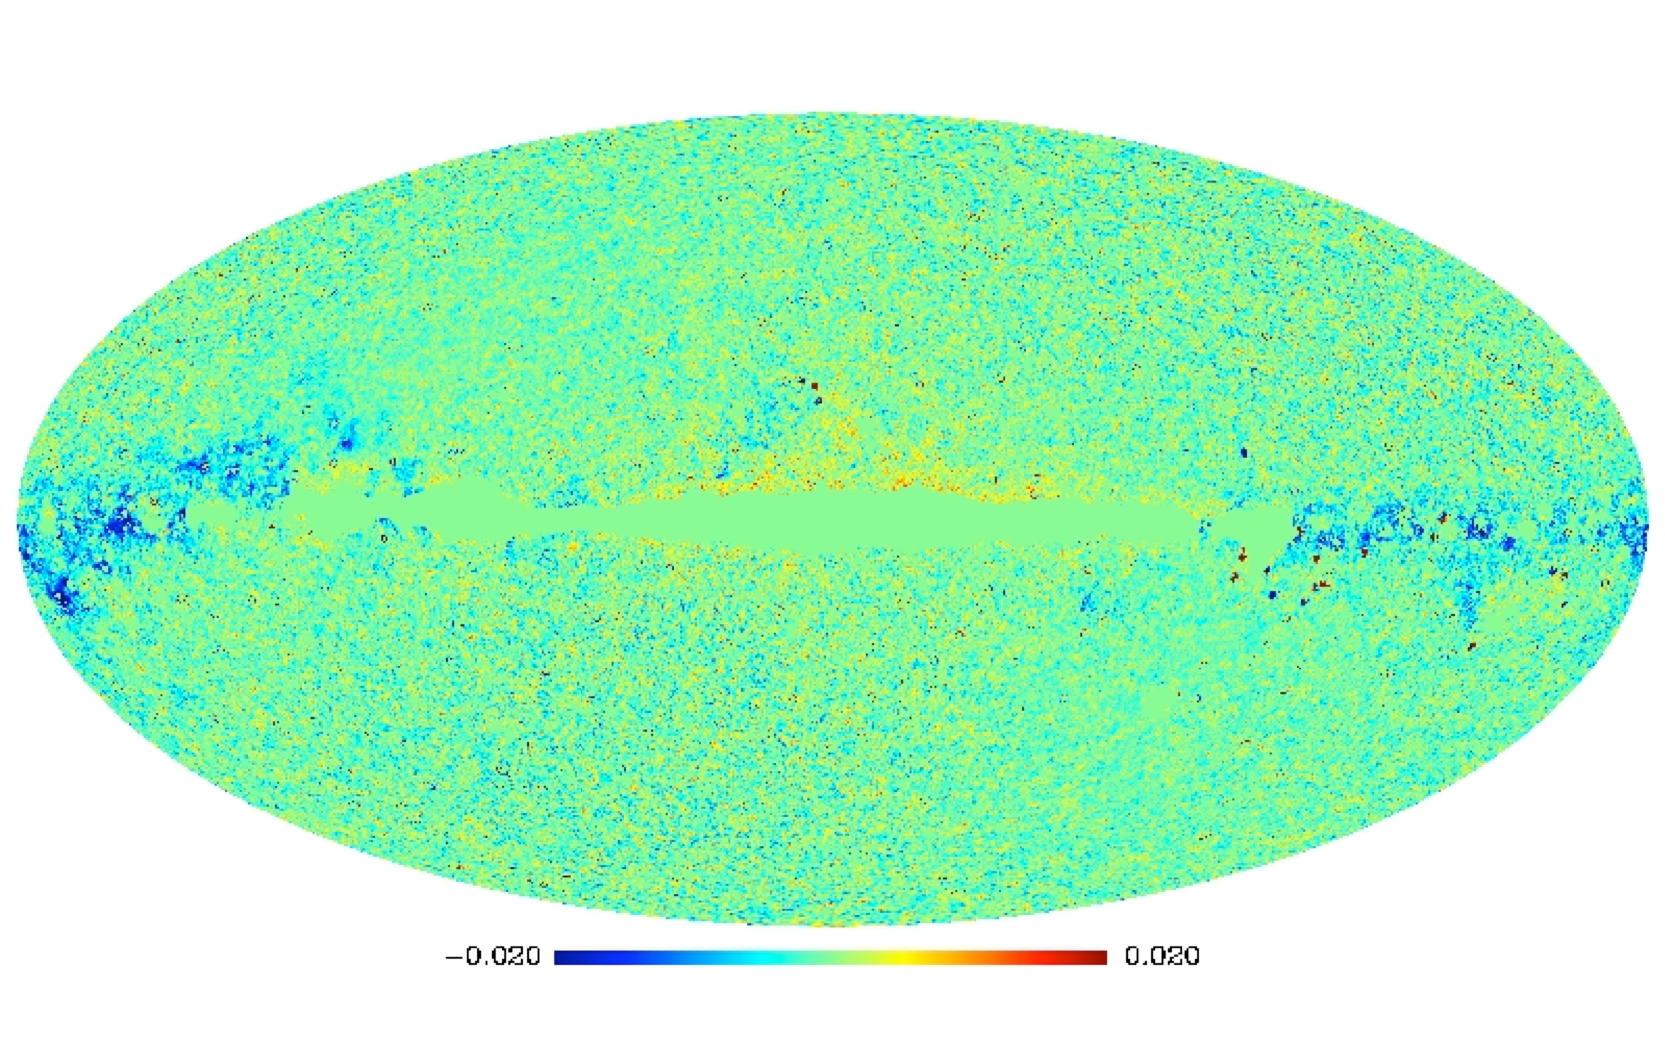
\includegraphics[width=12cm]{gmca_residual20_b.pdf} \\
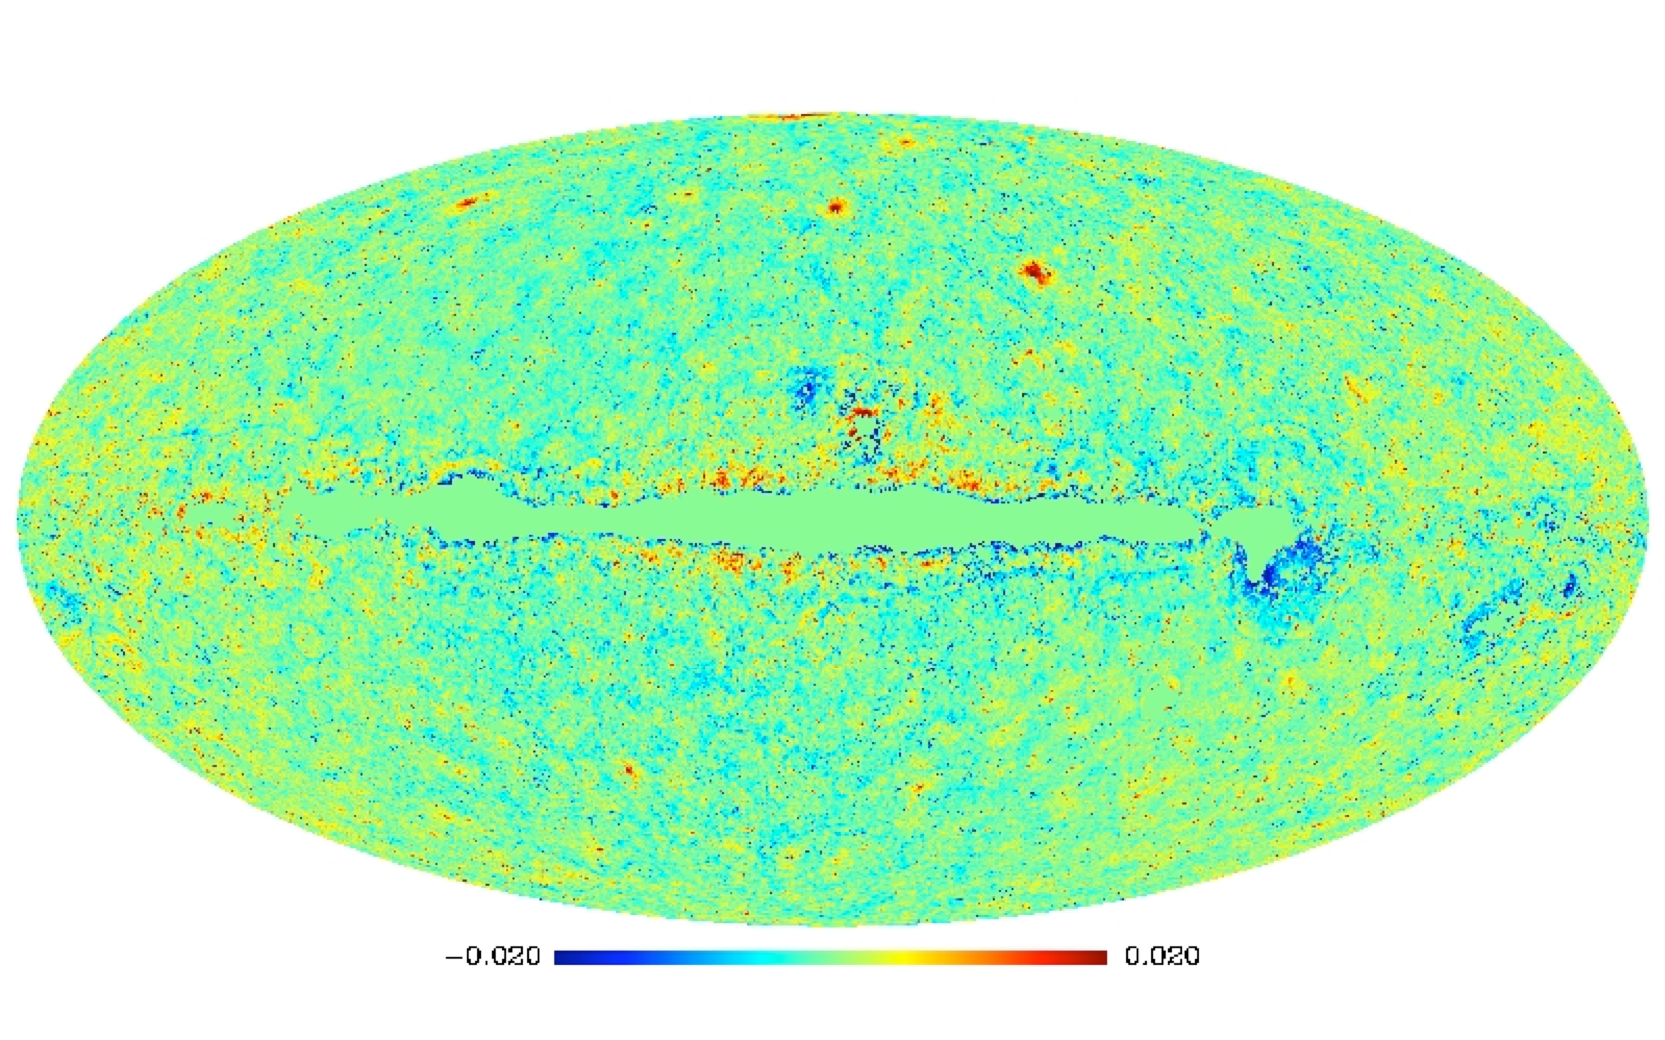
\includegraphics[width=12cm]{adamis_residual20_b.pdf} 
\end{array}
$$
\vspace{-0.1in}\caption{\textbf{Top~:} GMCA residual convolved at $20$ arcminutes. \textbf{Bottom~:} ADAMIS residual convolved at $20$ arcminutes. \textbf{Unit~:}  $10^{-3}$K.} \label{fig:wg2_resi20}
\end{figure}
\end{center}

\begin{center}
\begin{figure}[htb]
$$
\begin{array}{cc}
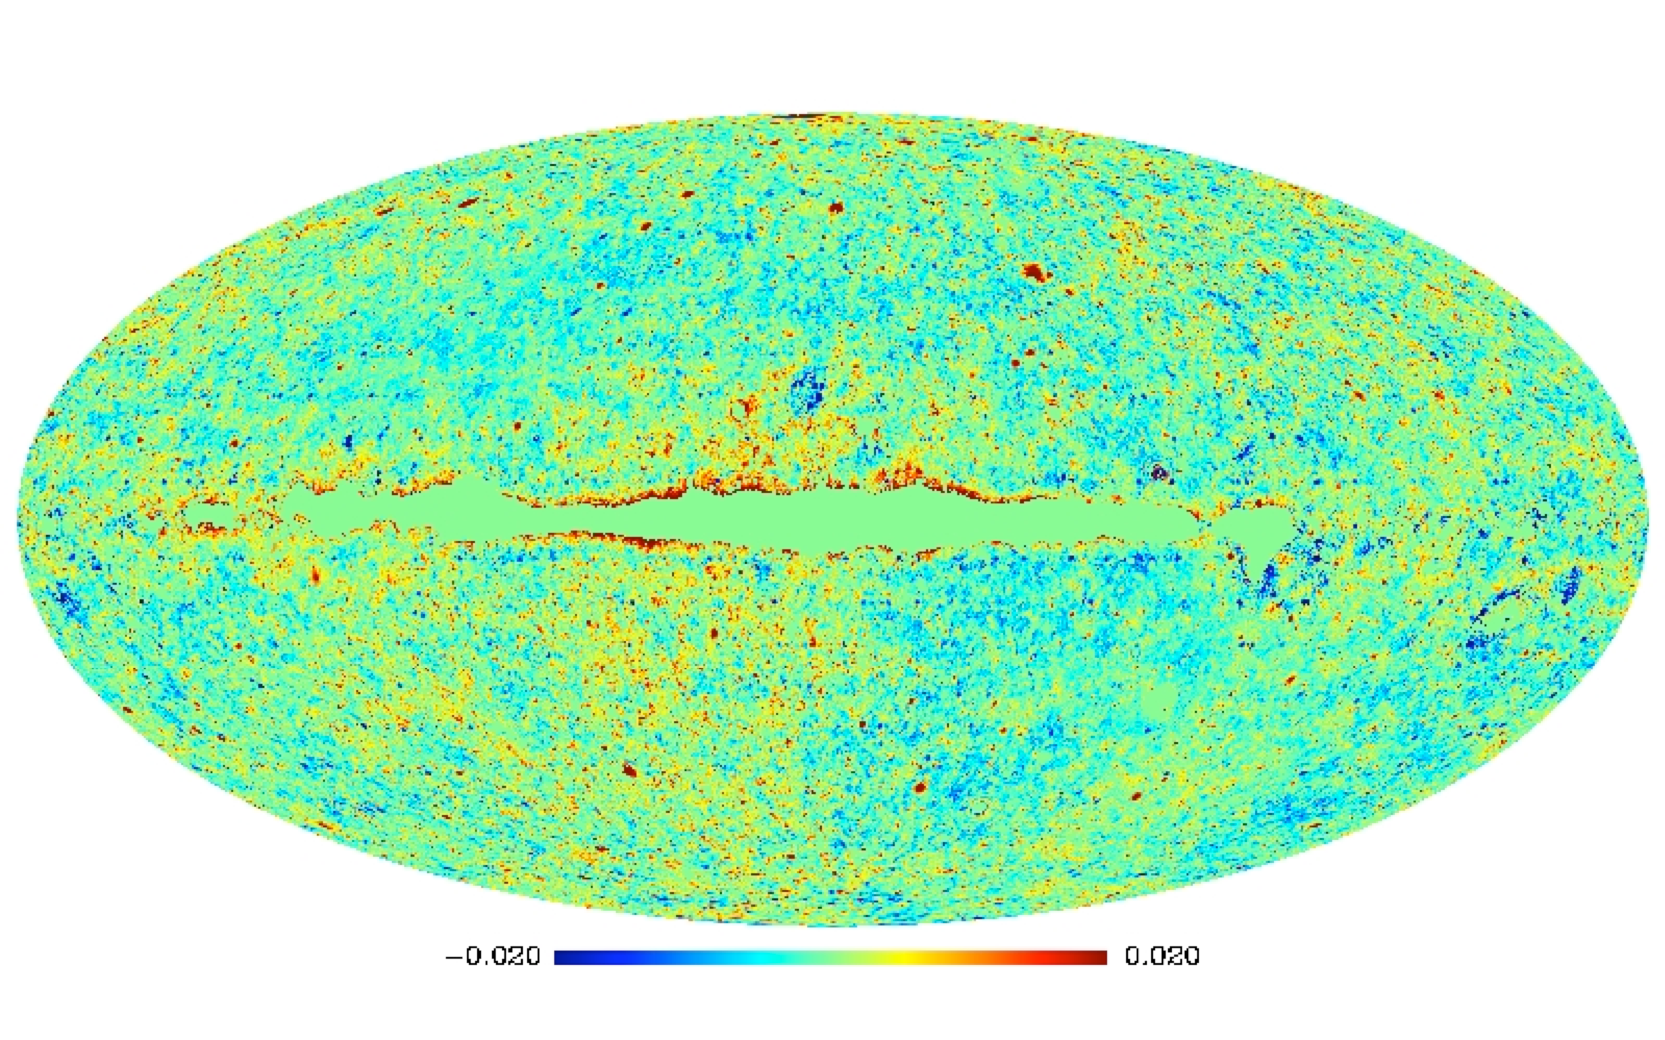
\includegraphics[width=12cm]{mem_residual20_b.pdf} \\
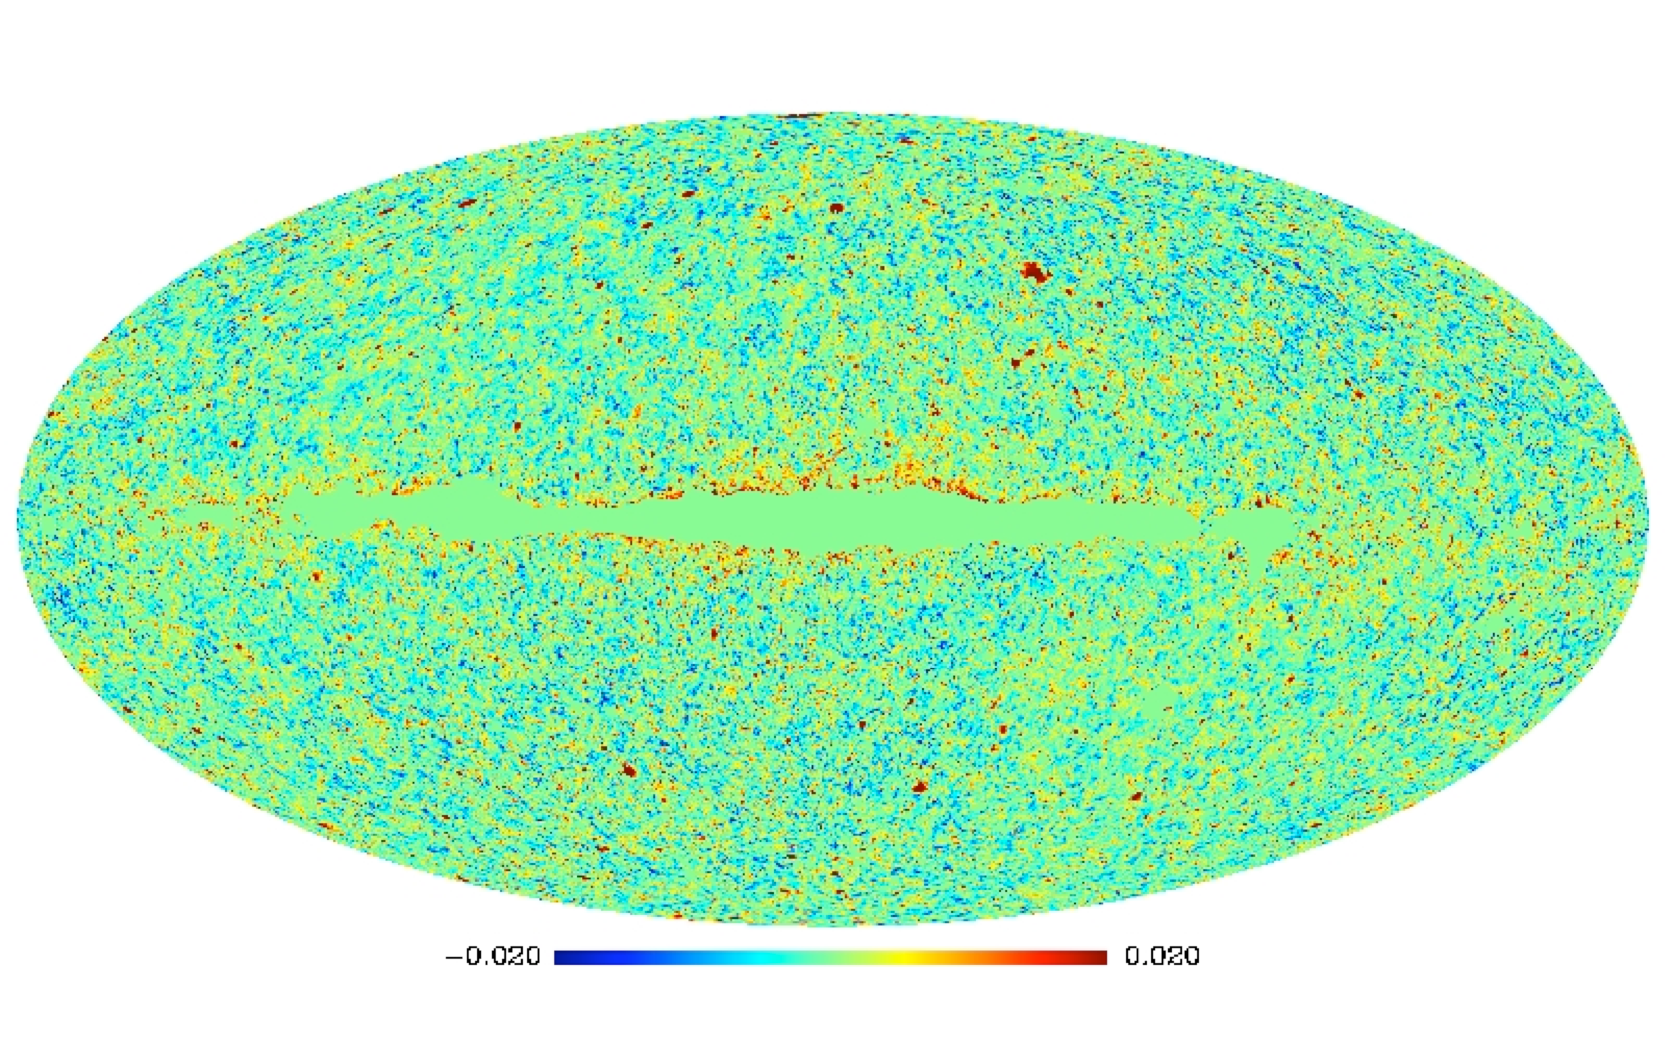
\includegraphics[width=12cm]{cca_residual20_b.pdf}
\end{array}
$$
\vspace{-0.1in} \caption{\textbf{Top~:} MEM residual convolved at $20$ arcminutes. \textbf{Bottom~:} CCA residual convolved at $20$ arcminutes. \textbf{Unit~:}  $10^{-3}$K.} \label{fig:wg2_resi20_2}
\end{figure}
\end{center}

\begin{center}
\begin{figure}[htb]
$$
\begin{array}{cc}
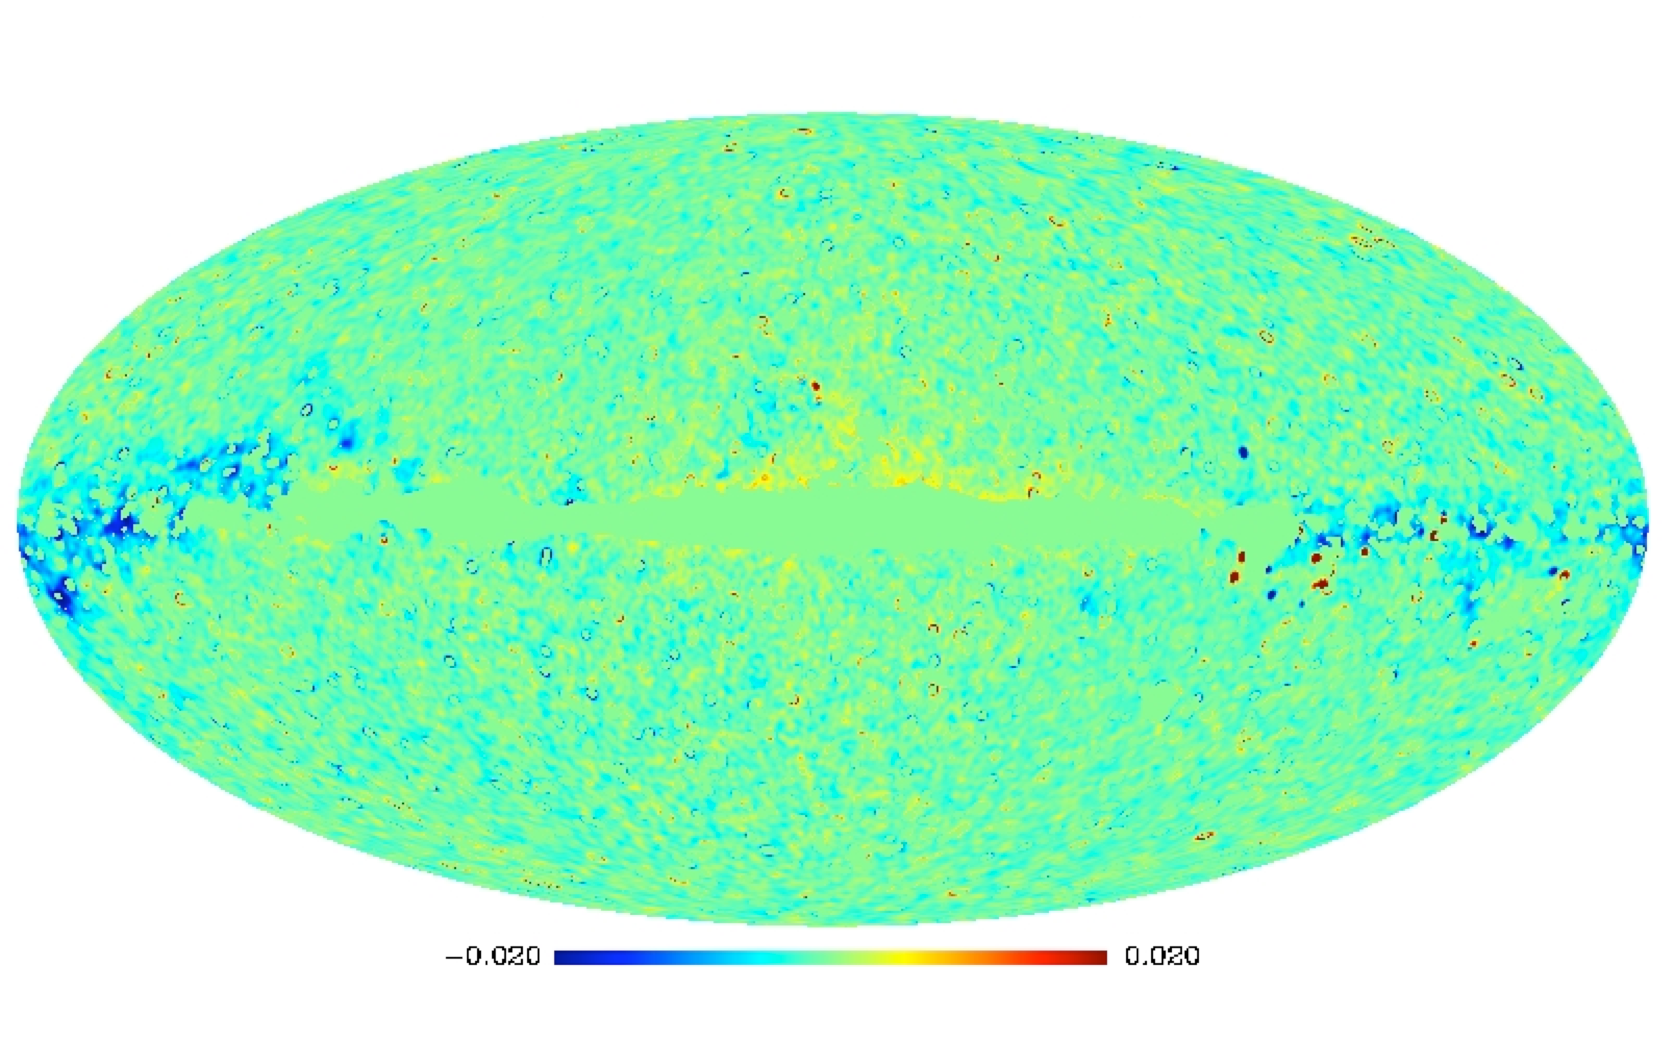
\includegraphics[width=12cm]{gmca_residual60_b.pdf} \\
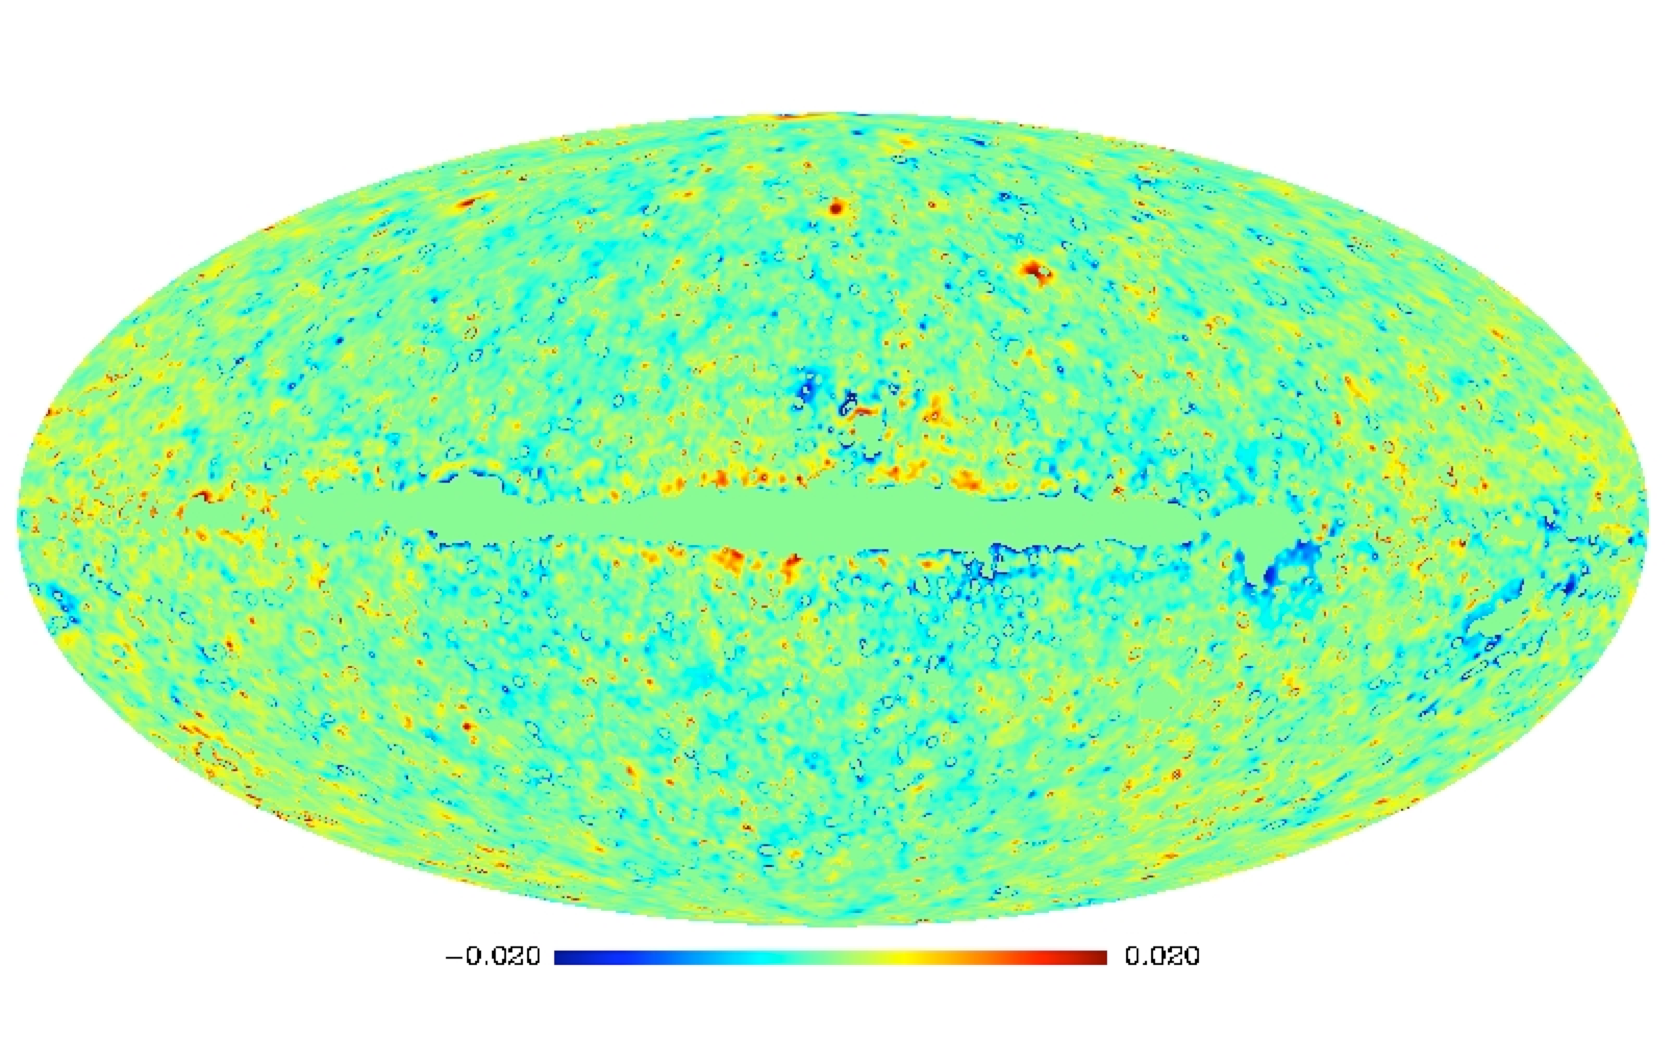
\includegraphics[width=12cm]{adamis_residual60_b.pdf} 
\end{array}
$$
\vspace{-0.1in} \caption{\textbf{Top~:} GMCA residual convolved at $60$ arcminutes. \textbf{Bottom~:} ADAMIS residual convolved at $60$ arcminutes. \textbf{Unit~:}  $10^{-3}$K.} \label{fig:wg2_resi60}
\end{figure}
\end{center}

\begin{center}
\begin{figure}[htb]
$$
\begin{array}{cc}
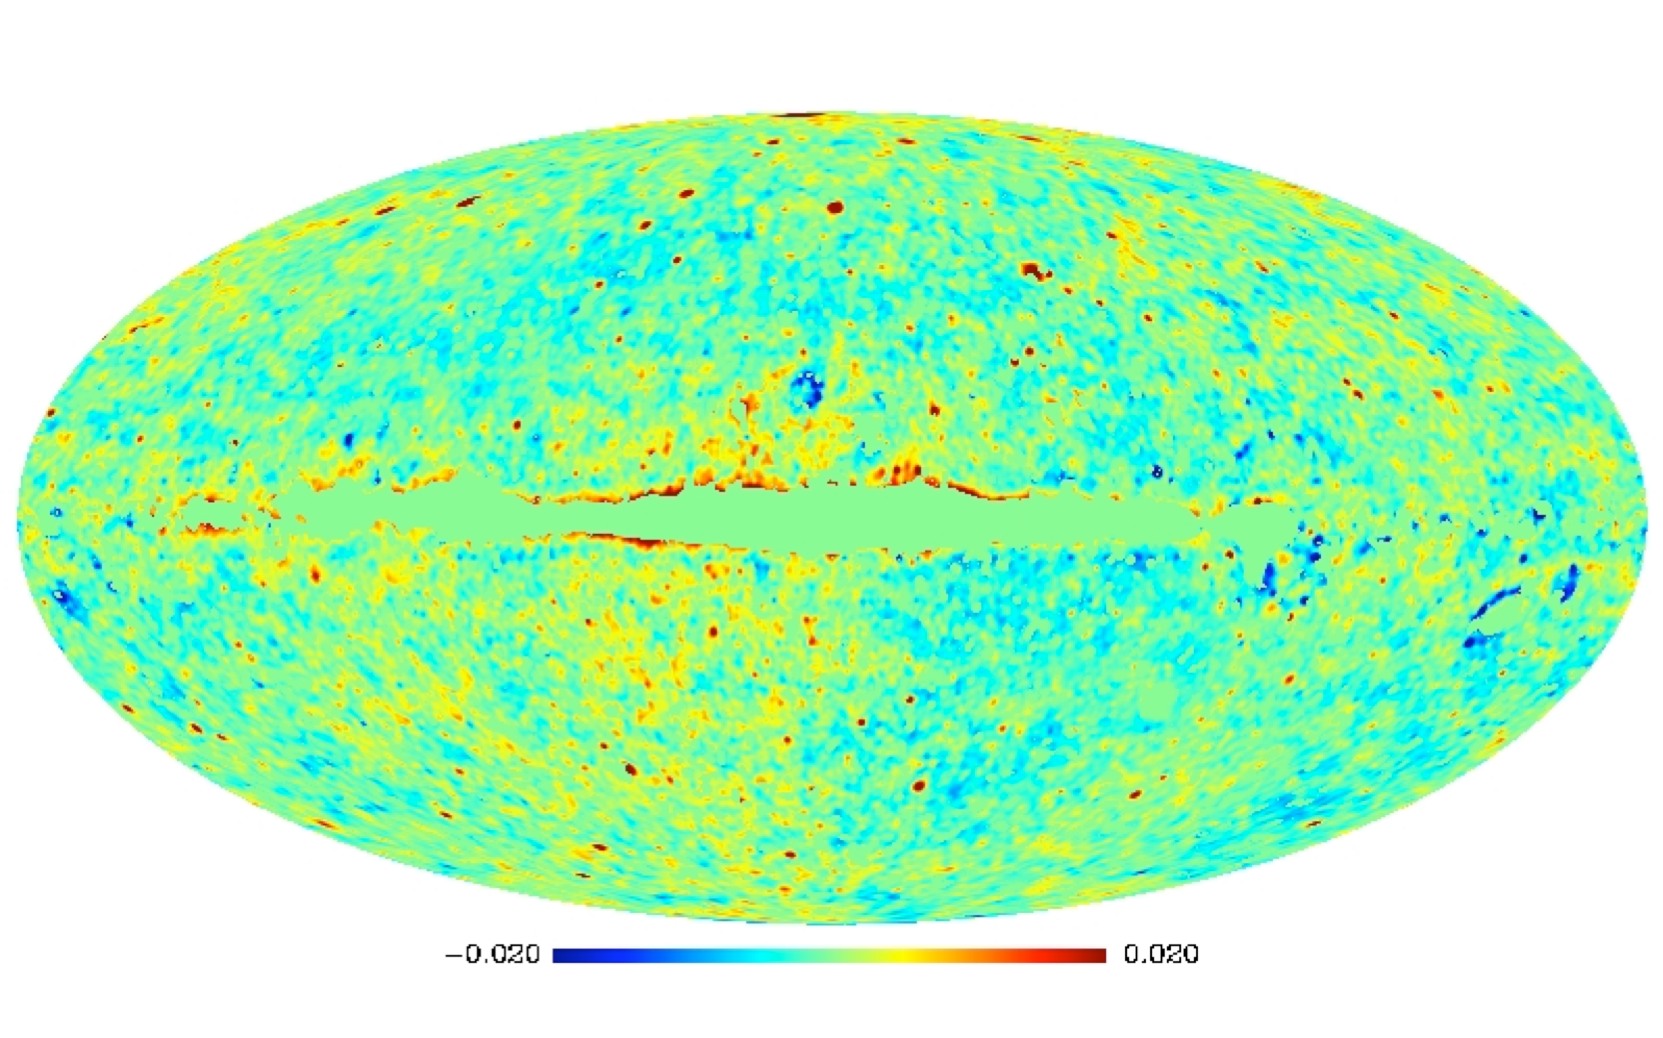
\includegraphics[width=12cm]{mem_residual60_b.pdf} \\
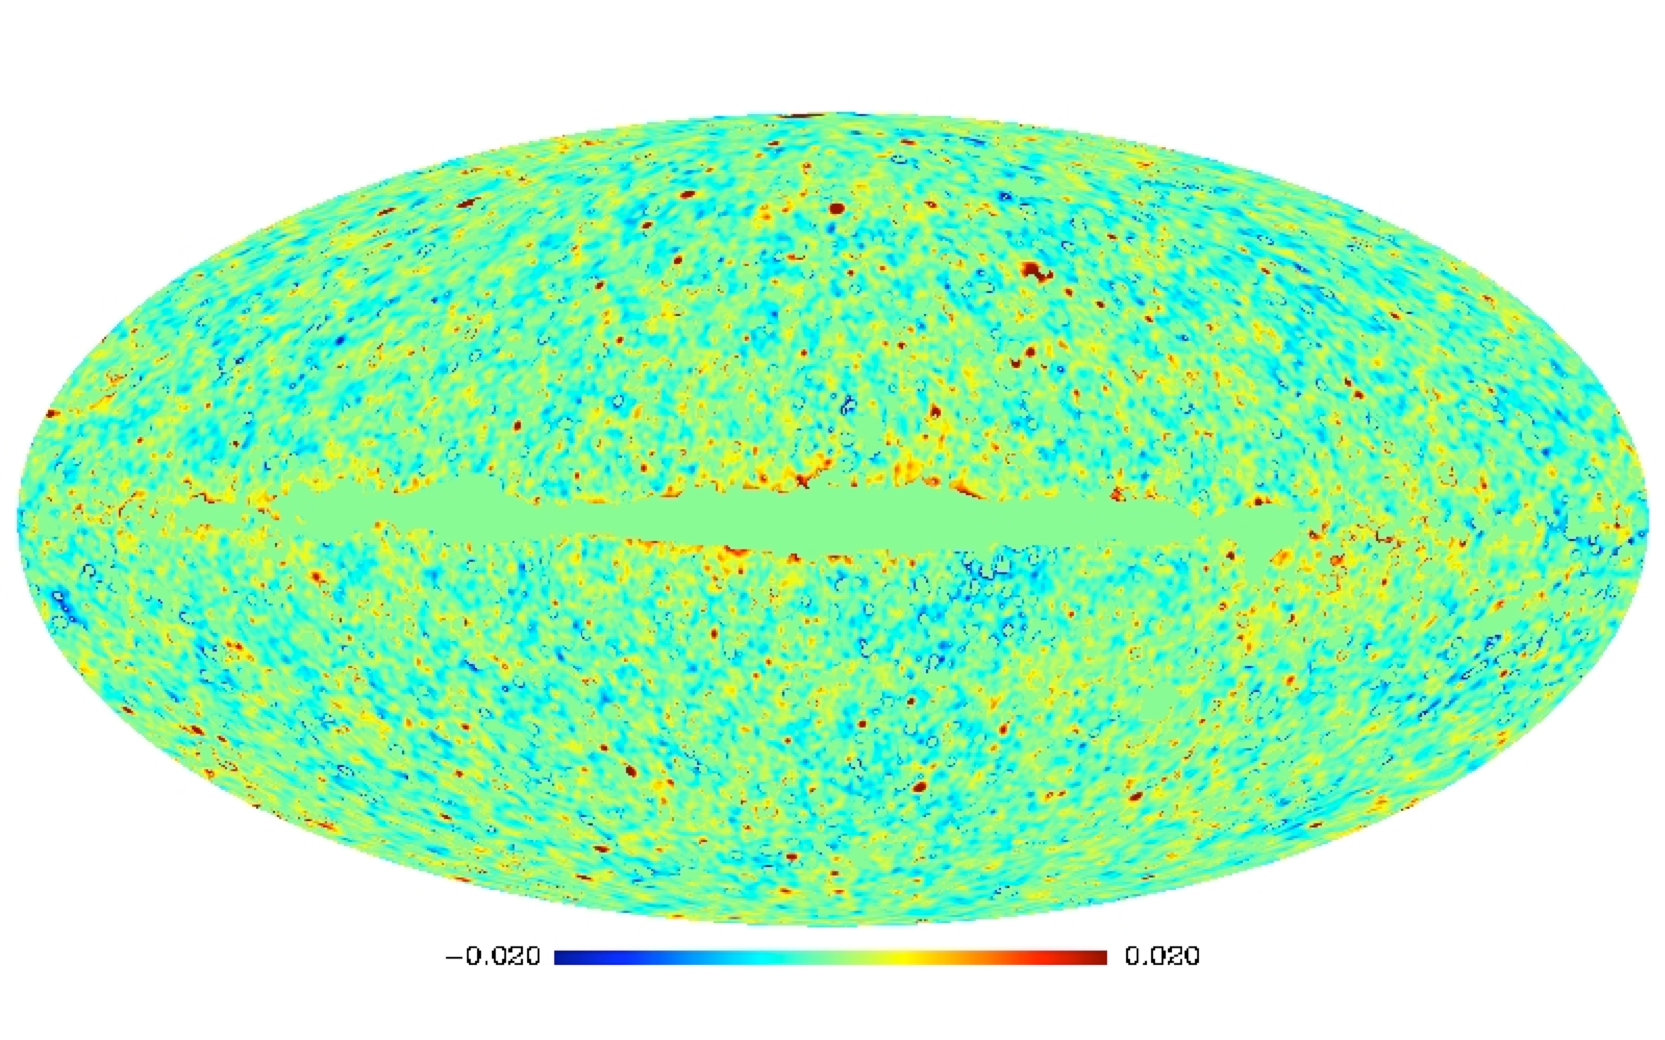
\includegraphics[width=12cm]{cca_residual60_b.pdf}
\end{array}
$$
\vspace{-0.1in} \caption{\textbf{Top~:} MEM residual convolved at $60$ arcminutes. \textbf{Bottom~:} CCA residual convolved at $60$ arcminutes. \textbf{Unit~:}  $10^{-3}$K.} \label{fig:wg2_resi60_2}
\end{figure}
\end{center}

\begin{figure}[htb]
\hspace{0.1in}
$$
\begin{array}{c}
%\begin{minipage}[b]{1\linewidth}
    \centerline{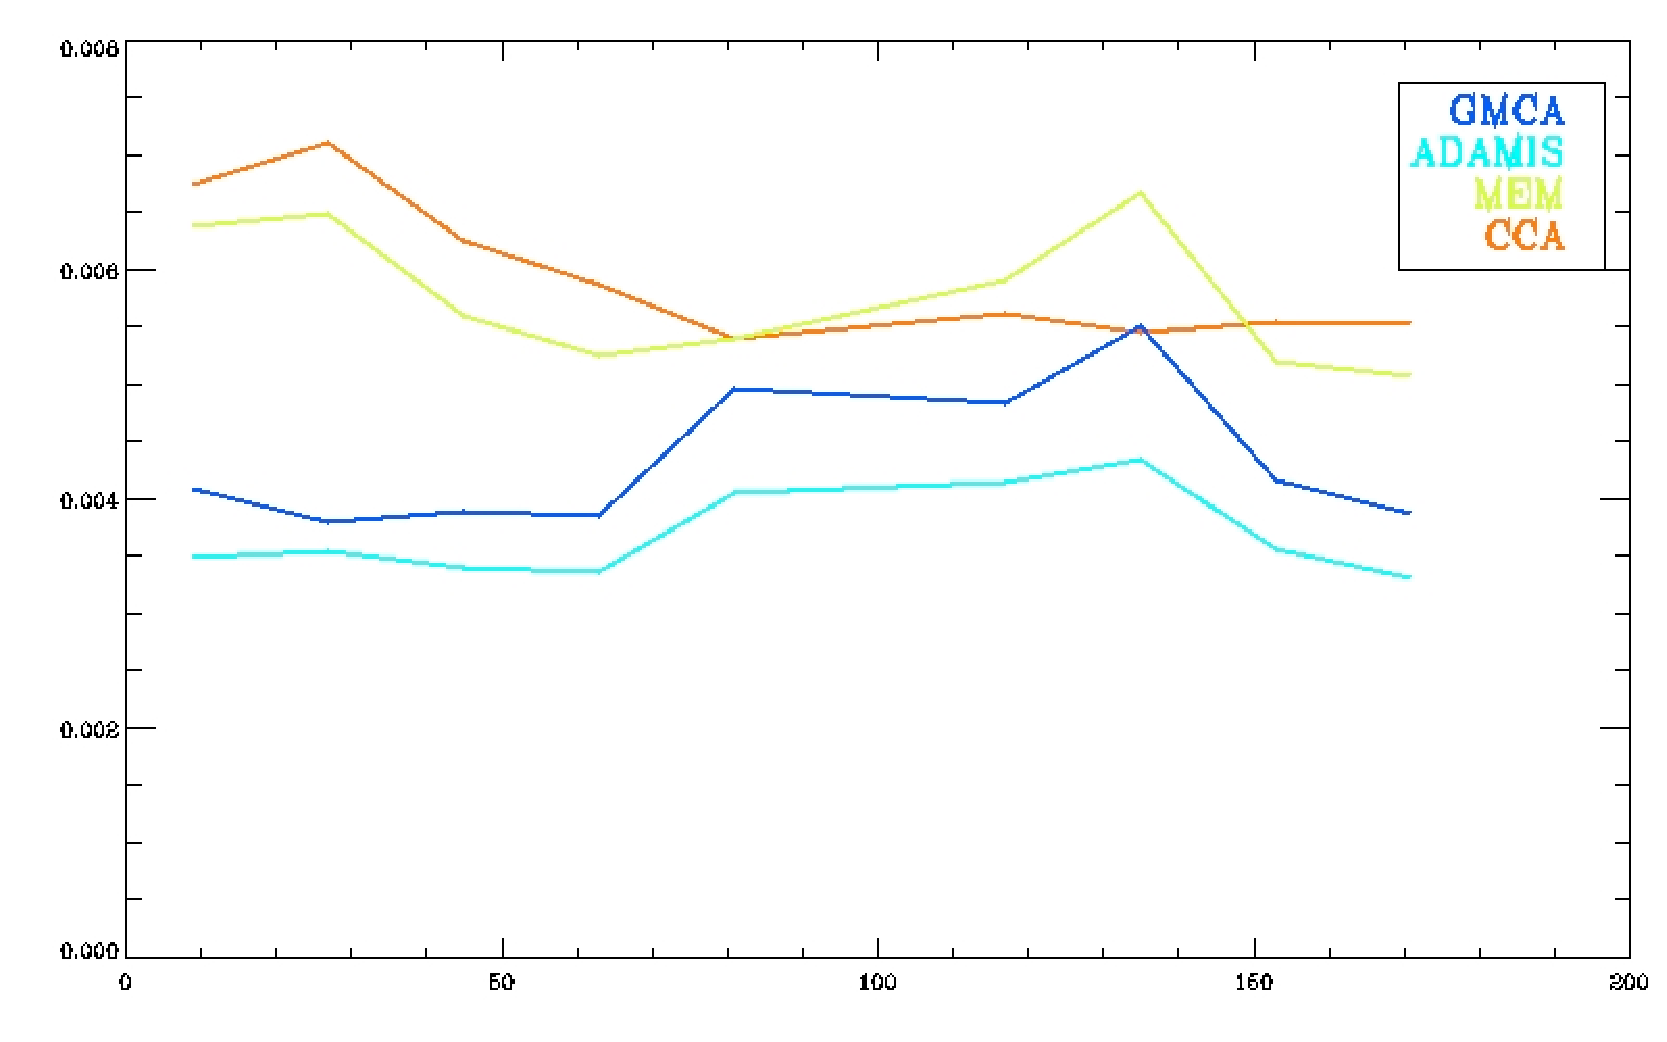
\includegraphics[width=12cm]{Residual_per20deg_20arcm.pdf}} \\
%\end{minipage}
%\vfill
%\begin{minipage}[b]{1\linewidth}
    \centerline{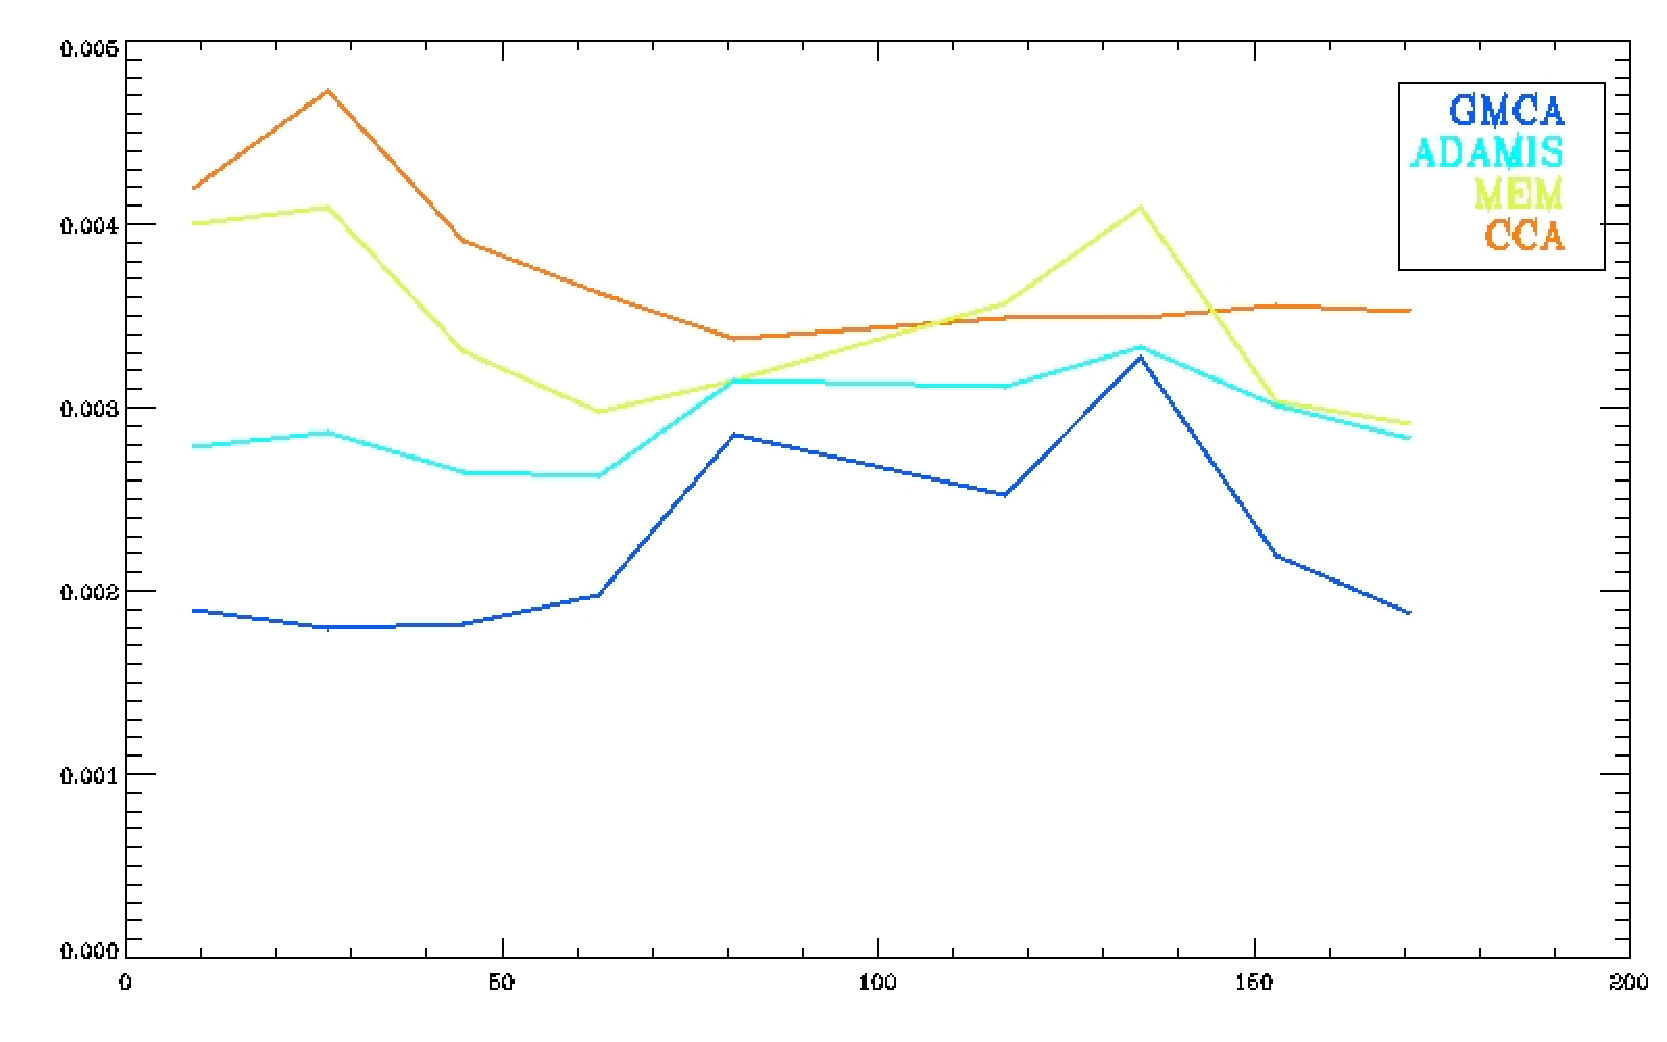
\includegraphics[width=12cm]{Residual_per20deg_60arcm.pdf}}
%\end{minipage}
\end{array}
$$
\vspace{-0.1in} 
\caption{\textbf{Top~:} standard deviation of the residual convolved at $20$ arcminutes per latitude bands with a width of $20^\circ$.\textbf{Bottom~:} standard deviation of the residual convolved at $60$ arcminutes per latitude bands with a width of $20^\circ$. \textbf{Abscissa~:} central latitude. The band centered in $90^\circ$ is not plotted. \textbf{Up~:} standard deviation of the residual in mK.}  \label{fig:wg2_resiperlat}
\end{figure}
E 2

D 2
 
E 1
E 2
